\documentclass[11pt,fullpage]{book}
\title{\textbf{~~~~~~~~~~~~~~~}\newline Bayesian book}
\author{Ben Lambert}
\usepackage{natbib}
\usepackage{appendix}
\usepackage{url,times}
\usepackage{graphicx}
\usepackage{epstopdf}
\usepackage{amsmath}
\usepackage[all]{xy}
\usepackage{pxfonts}
\usepackage{colortbl}
\usepackage{color}
\usepackage{subfigure}
\usepackage{gensymb}
\usepackage{ctable}
\usepackage[justification=centering]{caption}[2007/12/23]
\usepackage{longtable}
\usepackage{pstricks-add}
\usepackage{pstricks}
\usepackage{pst-func}
\usepackage{pst-math}



\setlength{\parindent}{0.0in}
\setlength{\parskip}{0.1in}
\maketitle

\begin{document}
\tableofcontents


\chapter{How to best use this book}



\part{Understanding the Bayesian formula}

\chapter{The subjective worlds of frequentist and Bayesian statistics}
\section{Chapter mission statement}
At the end of this chapter the reader will understand the similarities and differences between frequentist and Bayesian statistics. Furthermore, the reader will gain knowledge about probability distributions, as well as how they can be manipulated to calculate quantities of interest. Finally, we discuss the benefits of using Bayesian statistics for a particular analysis.
 
\section{Chapter goals}
When we wish to 

\section{The purpose of statistical inference}
What is the benefit of a particular drug to treatment success? What is the return on a college education? Will the Democrats win the next US Presidential election? We frequently in life want to test theories, and go on to draw conclusions about processes of interest.

However, it is often impossible to exactly isolate the parts of a system which we want to examine. The outcome of history is hence determined by a nexus of interacting elements; each of which contributes to the reality that we witness. In the case of a drug trial, we may not be able to control the diets of participants, and are certainly unable to control for their idiosyncratic metabolisms, both of which could impact the results we see. Evaluating the return to a college education - there are a range of factors which affect the wage which an individual ultimately commands, of which education is only one element. The outcome of the next US Presidential election depends on party politics, the performance of the incumbent government, as well as the media's portrayal of the candidates. 

In life noise obfuscates the signal. The wind, rain, sleet and snow make it difficult to forge a path to where we want to go.

Statistical inference allows us to draw conclusions in this blustery landscape; separating the signal from the noise. It is the logic which means we can trial our beliefs against \textit{data}. 

In statistics, we formalise our beliefs in models of \textit{probability}. The models are probabilistic because we assume we are ignorant to most of the multitude of interacting parts of a system, meaning we cannot say with certainty whether something will, or will not, occur.

Suppose we are evaluating the efficacy of a drug in a trial. We might suppose that \textit{on average}, the drug might have a given probability of working as desired. However, before we carry out any trials, we are unaware of its exact treatment success rate. Fortunately, statistical inference allows us to estimate this unknown characteristic, or \textit{parameter}, from the data we are given. 

There are two schools of thought for carrying out this process of inference: \textit{frequentist} and \textit{Bayesian}. Although this book is devoted to the latter, we now spend some time comparing the two approaches, so that a reader is aware of the different paths taken to their shared goal.

\section{The world according to frequentists}
In frequentist or classical statistics, we suppose that our sample of data is the result of one of an infinite number of exactly-repeated experiments. The sample we see in this context is hence assumed to be the outcome of some probabilistic process. Any conclusions that we draw from this approach are based on the supposition that events occur with probabilities, which represent long-run frequencies. 

For example, if we flip a coin, we might assume that any sequence of outcomes we obtain is indicative of the results that we might obtain if we were to conduct the experiment an infinite number of times. Further, we might take the proportion of heads observed in this infinite set of throws as defining the probability of obtaining a 'heads'. We suppose that this probability actually exists, and is fixed for each set of coin-throws that we carry out.

In general, in frequentist statistics assume that the data is \textit{random} and results from \textit{sampling}, from a fixed and defined \textit{population} distribution. For a frequentist the noise that obscures the true signal of the population relationship in which we are interested is due to \textit{sampling variation}; the fact that the sample that we pick will each time be slightly different, and not exactly representative of the population. 

We may flip our coin 10 times, obtaining 7 heads even if the long-run proportion of heads is $\frac{1}{2}$. To a frequentist, this is because we have picked a slightly odd sample from the population of infinitely-many repeated throws. Further, if we flip the coin another 10 times, we will likely get a different result, because we have picked a different sample.

\section{The world according to Bayesians}
Bayesians do not imagine repetitions of an experiment in order to define and specify a probability. It is merely taken as a measure of certainty of a particular belief. From this viewpoint, the probability of us throwing a 'heads' measures and quantifies our underlying belief, that before we flip the coin, it will land this way. 

In this sense, Bayesians do not view probabilities as concrete entities that actually exist. They are merely abstractions which we can use to help express our uncertainty. In this frame of reference there is no necessity for events to be repeatable in order to define a probability. We are thus equally able to say, 'The probability of a heads is 0.5', or, 'The probability of the democrats winning the 2020 US Presidential election is 0.75'. Probability is merely seen as a scale from: 0 where we are certain an event will not happen, to 1 where we are certain it will. 

A statement such as 'The probability of the democrats winning the 2020 US Presidential election is 0.56' is hard to explain using the frequentist definition of a probability. There is only ever one possible sample - the history that we witness - and what would we actually mean by a 'population of all possible US elections which happen in the year 2020'? 

Probabilities are therefore seen as an expression of subjective beliefs, meaning they can be updated in light of new data. The formula invented by the Reverend Thomas Bayes provides the \textit{only} logical manner in which to carry out this process, and is central to Bayesian inference, where we aim to express probabilistically our uncertainty in parameters after we have seen the \textit{data}. 

Bayesians assume, since we are witness to the data, that it is \textit{fixed}, and therefore does not vary. We do not need to imagine that there are an infinite number of possible samples. We 'see' our data, and hence do not need to view it as the outcome of some random process.

In contrast, we do not ever learn exactly the value of an unknown parameter. This epistemic uncertainty means that in Bayesian inference we choose to view the parameter as a quantity that is probabilistic in nature. We can view this in one of two perspectives. Either we view the unknown parameter as truly being \textit{fixed} in some absolute sense, but our beliefs are uncertain, and thus probabilistic. Alternatively, we can take the view that there isn't some definitive \textit{population} process, and for each sample we take, we get a slightly different parameter.

In the latter perspective we get different results from the coin flipping because each time we are subjecting our system to a slightly different probability of it landing 'heads' up. This could be because we mildly altered our throwing technique, or started with the coin in a different position. In the former perspective, we view the sample as a noisy representation of the signal, and hence we get different results for each set of throws.

Although these two descriptions are different philosophically, they are not mathematically, meaning we can apply the same analysis to both.

\section{Frequentist and Bayesian inference}
The Bayesian inference process is the only logical way to modify our beliefs to take into account new data. We start out before we collect data with a probabilistic description of our beliefs, which we call a \textit{prior}. We then collect data, and together with a model describing our theory, Bayes' formula for probability allows us to calculate our post-data or \textit{posterior} belief:

\begin{equation}
prior + data \xrightarrow{model} posterior
\end{equation}

In Bayesian inference, we want to draw conclusions based on purely probabilistic descriptions of phenomena. If we wish to summarise our evidence for a particular hypothesis, we describe this probabilistically, as the 'probability of the hypothesis \textit{given} the data obtained'. 

The difficulty in obtaining this type of conclusion is that when we write down a probability model describing our process of interest, we can only use it to compute the 'probability of obtaining our data \textit{given} our hypothesis being true'. Frequentists stop here. Using this probability as evidence for a particular hypothesis in question. If the probability of obtaining data\footnote{Actually technically obtaining a result as or more extreme than the data.} given a hypothesis is small, then we reject the hypothesis in question.

Bayesians allow inversion of this probability.

Diagram explaining the difference between Bayesians and frequentists.

\subsection{Locating a submarine: example}

\section{Probability distributions: helping us explicitly state our ignorance}\label{sec:Intro_probabilityDistributions}
Before we look out the window in the morning, before we get our exam results, before the cards are dealt, we are uncertain of the world that lies in wait of us. In order to plan, as well as make sense of things, we frequently implicitly formulate an idea as to the relative likelihood of different outcomes. However, in order to allow interrogation of thought, with a view to transparency and self-improvement, we sometimes would like to state our pre-conceptions \textit{explicitly}, in the form of a suitable framework. 

The mathematical theory of probability provides a logic and language which is suitable to describe the majority of cases in which we are uncertain. Imagine that before we roll a die - which we believe to be fair - we assign an equal probability of $\frac{1}{6}$ to each of six the possible outcomes. Although we haven't stated this world-view in mathematical notation, we have without realising it, formulated a valid probability distribution\footnote{This is technically a probability mass function, since we are describing a discrete random variable, but we prefer to not differentiate terminology.} for the number shown on the die (see figure \ref{fig:Intro_die}). 

\begin{figure}
\centering
\scalebox{0.65} 
{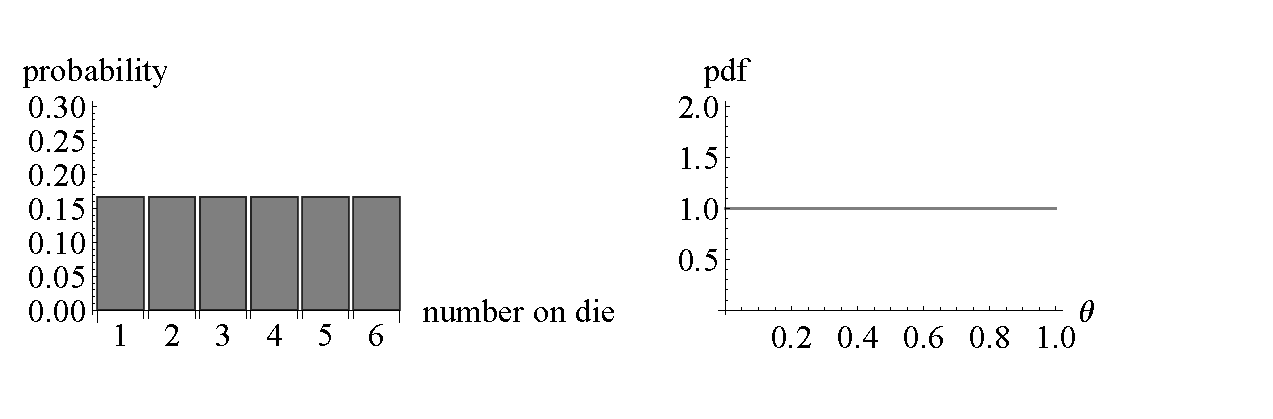
\includegraphics{Intro_die.pdf}}
\caption{Left) A discrete uniform probability distribution for the number shown on a rolled fair die. Right) A continuous distribution to represent the probability of a coin coming up heads, $\theta$.\textbf{I want to remove the ticks from the discrete plot, simply placing a $\frac{1}{6}$ there instead.}}\label{fig:Intro_die}
\end{figure}

\subsection{What make a probability distribution \textit{valid}? The most important thing today}\label{sec:Intro_validProbabilityDistribution}
The die example given in section \ref{sec:Intro_probabilityDistributions} refers to discrete probability distribution, since the variable we were measuring - the number shown on the die after a throw - is confined to take on finite set of values. However, we could similarly define a probability distribution where our variable is able to take on an infinity of values across a spectrum. Before we flip a coin we might be uncertain as to its innate bias, and might\footnote{Perhaps foolishly since typically we expect that coins are designed to be relatively \textit{fair} in this respect.} imagine that any value for the probability of it coming up heads, $\theta$, is equally likely. This results in the \textit{continuous} analogue of the discrete die example (see figure \ref{fig:Intro_die}).

The aforementioned examples are both examples of valid/proper probability distributions. So, what are its defining properties?

\begin{itemize}
\item All values of the distribution must be real, and non-negative.
\item The sum (integral) across all possible values of the discrete (continuous) random variable must be 1.
\end{itemize}

In the die case, this is satisfied since $p(X)=\frac{1}{6}\geq 0$, and:

\begin{equation}
\sum\limits_{i=1}^{6} \frac{1}{6} = 1
\end{equation}

For the continuous case of the probability of a heads when flipping a coin, the probability density function is always $1\geq0$, and when we do the continuous analogue of summing - integrating - we find that:

\begin{equation}
\begin{align}
\int\limits_{0}^{1} p(\theta) \mathrm{d}\theta &= \int\limits_{0}^{1} 1 \mathrm{d}\theta\\
&= 1
\end{align}
\end{equation}

Although, it may seem that this definition is relatively arbitrary, and perhaps well-trodden-territory for some readers, it is of \textit{central} importance to Bayesian statistics. This is because Bayesians like to work with, and produce \textit{valid} probability distributions. The pursuit of this ideal underlies the majority of \textit{all} methods in applied Bayesian statistics - analytic and computational - and hence its importance cannot be overstated!

\subsection{Interpreting discrete and continuous probability distributions}
The discrete probability distribution for a fair die shown on the left hand side in figure \ref{fig:Intro_die}, is straightforward to interpret. To calculate the probability that the die lands on a 1, we simply read off the probability from the graph corresponding to the height of the leftmost bar, and find that:

\begin{equation}
p(X=1)= \frac{1}{6}
\end{equation}

In the discrete case, if we want to calculate the probability that a random variable takes on a range of values, then we simply need to sum the individual probabilities corresponding to each specific event. In the die example, if we want to calculate the probability that the die lands on a number less than 4, we just add together the probabilities of it landing on 1, 2 and 3:

\begin{equation}
\begin{align}
p(X<4) &= p(X=1) + p(X=2) + p(X=3)\\
&= \frac{1}{6} + \frac{1}{6} + \frac{1}{6}\\
&= \frac{1}{2}
\end{align}
\end{equation}

How can we use the continuous probability distribution such as the one shown on the right hand side of figure \ref{fig:Intro_die}? If we want to calculate the probability that the bias of the coin is zero, in other words, the probability that $\theta=0.5$, then we could simply draw a vertical line from this point on the $\theta$ axis up to the line of the distribution; concluding that $p(\theta=0.5) = 1$! We know that this is not the intended result, since we supposed before that \textit{all} values of $\theta$ were equally likely. This means that the probability that $\theta$ takes on any particular value between 0 and 1 is \textit{actually} zero. Intuitively, this is because there are an infinity of particular values between 0 and 1 which $\theta$ can feasibly take on, meaning that picking one of them is infinitely unlikely. For example, the following values $\theta=\{0.5,0.501,0.50001,0.5000001\}$ are all equally likely, and we could generate an infinity of these test values of $\theta$, meaning that each one must have a zero likelihood of occurring. This means for a continuous random variable, we always have $p(\theta=number) = 0$. Hence, when we write $p(\theta)$ for a continuous random variable, we should be careful to interpret the value of it at a particular value as a probability \textit{density}, \textit{not} a probability. 

However, we can use a continuous probability distribution to calculate the probability that a random variable lies between two bounds. To do this we use the continuous analogue of a sum, an \textit{integral}. For the coin example, we can hence calculate the probability that $0.25\leq \theta \leq 0.75$:

\begin{equation}\label{eq:Intro_continuousProbabilityIntervalExample}
\begin{align}
Pr(0.25\leq \theta \leq 0.75) &= \int\limits_{0.25}^{0.75} p(\theta) \mathrm{d}\theta\\
&= \int\limits_{0.25}^{0.75} 1 \mathrm{d}\theta\\
&= \left[\theta\right]^{0.75}_{0.25} = (0.75-0.25) = 0.5
\end{align}
\end{equation}

In (\ref{eq:Intro_continuousProbabilityIntervalExample}), we have used $Pr$ to explicitly state that the result is a \textit{probability}, whereas $p(\theta)$ is a probability density. Of course, the calculation carried out in (\ref{eq:Intro_continuousProbabilityIntervalExample}), is equivalent to working out the area under the graph within those limits (see figure \ref{fig:Intro_continuousInterval}).

\begin{figure}
\centering
\scalebox{0.5} 
{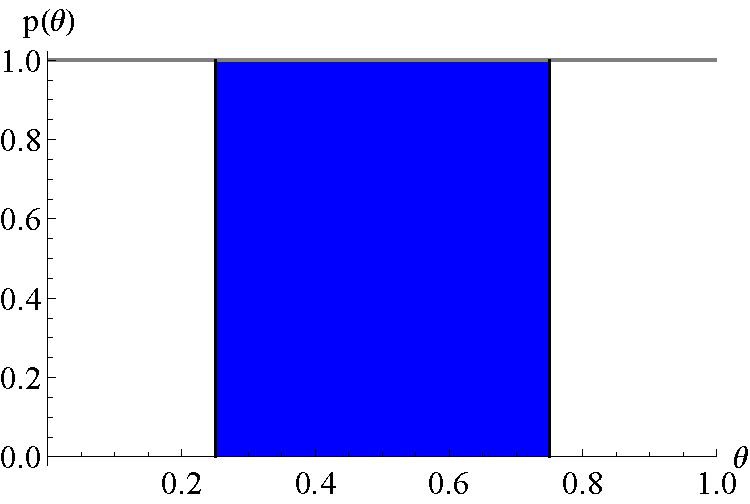
\includegraphics{Intro_continuousInterval.pdf}}
\caption{The probability that $\theta$, representing the probability that a heads is thrown, lies between 0.25 and 0.75.}\label{fig:Intro_continuousInterval}
\end{figure}

\subsection{Mean and variance of distributions}
Often presentation of a distribution as a result in itself is interesting mainly due to the value of its summary measures. A popular way of summarising a distribution is via its \textit{mean}, which is one measure of central tendency of a distribution. More intuitively, a mean, or \textit{expected value}, of a distribution represents the long-run average value that would be obtained if we sampled from that particular distribution in question, an infinite number of times. 

The way in which we calculate the \textit{mean} of a distribution depends on whether it is \textit{discrete} or \textit{continuous} in nature. However, the concept is essentially the same in both cases. The mean is calculated as a weighted sum of the values taken on by the random variable in question, where the weights are provided by the probability distribution. This results in the following forms for the mean of a discrete and continuous variable respectively:

\begin{equation}\label{eq:Intro_meanDistributionDiscrete}
\mathbb{E}(X) = \sum\limits_{All\; \alpha} \alpha Pr(X=\alpha)
\end{equation}

\begin{equation}\label{eq:Intro_meanDistributionContinuous}
\mathbb{E}(X) = \int\limits_{All\; \alpha} \alpha p(\alpha)\mathrm{d}\alpha
\end{equation}

In (\ref{eq:Intro_meanDistributionDiscrete}) and (\ref{eq:Intro_meanDistributionContinuous}), $\alpha$ represents the multitude, or continuum of \textit{values} taken on by the random variable $X$ respectively.  We have chosen to use $Pr$ in (\ref{eq:Intro_meanDistributionDiscrete}), and $p$ in (\ref{eq:Intro_meanDistributionContinuous}), to illustrate that these represent probabilities and probability \textit{densities} respectively.

We can now apply (\ref{eq:Intro_meanDistributionDiscrete}) to allow us to calculate the mean of the fair die distribution shown in the left-hand panel of figure \ref{fig:Intro_die}:

\begin{equation}\label{eq:Intro_meanFairDie}
\begin{align}
\mathbb{E}(X) &= \sum\limits_{\alpha=1}^{6} \alpha Pr(X=\alpha)\\
&= 1\times\frac{1}{6} +  2\times\frac{1}{6} + 3\times\frac{1}{6} + 4\times\frac{1}{6} + 5\times\frac{1}{6} + 6\times\frac{1}{6}\\
&= 3\tfrac{1}{2}
\end{align}
\end{equation}

We can also demonstrate the \textit{long-run} nature of the mean value of $3\tfrac{1}{2}$ found in (\ref{eq:Intro_meanFairDie}) by simulating a number of rolls of a fair die computationally (see figure \ref{fig:Intro_meanDiscreteLongRun}). As the number of rolls increases, the running mean tends towards this value.

\begin{figure}
\centering
\scalebox{0.8} 
{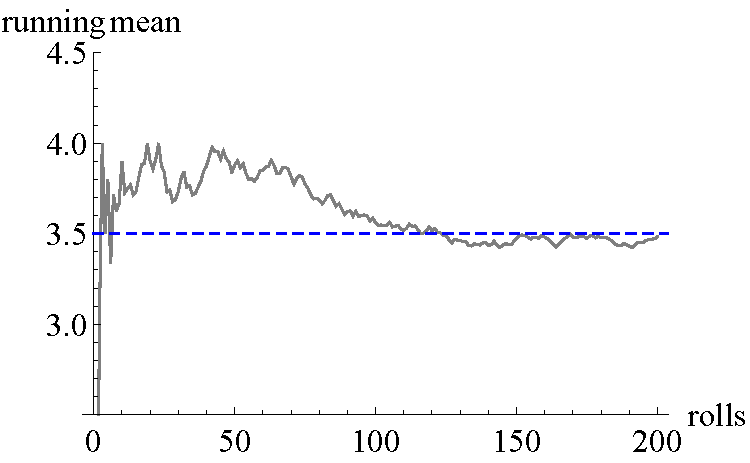
\includegraphics{Intro_meanDiscreteLongRun.pdf}}
\caption{Rolling a (computational) die. We show the running average for rolling a fair die a number of times.}\label{fig:Intro_meanDiscreteLongRun}
\end{figure}

We can also apply (\ref{eq:Intro_meanDistributionContinuous}) to calculate the mean of the uniform distribution representing our beliefs as to the bias of a flipped coin, shown in the right-hand side of figure \ref{fig:Intro_die}:

\begin{equation}\label{eq:Intro_meanCoinContinuous}
\begin{align}
\mathbb{E}(X) &= \int\limits_{0}^{1} \theta p(\theta)\mathrm{d}\theta\\
&= \left[\frac{\theta^2}{2}\right]^{1}_{0} = (\frac{1}{2}-0)\\ 
&= \frac{1}{2}
\end{align}
\end{equation}

Again, we can simulate the convergence of a running mean to the value of $\frac{1}{2}$ found in (\ref{eq:Intro_meanCoinContinuous}) by 'drawing' values of $\theta$ from this continuous uniform distribution a number of times (see figure \ref{fig:Intro_meanContinuousLongRun}).

\begin{figure}
\centering
\scalebox{0.8} 
{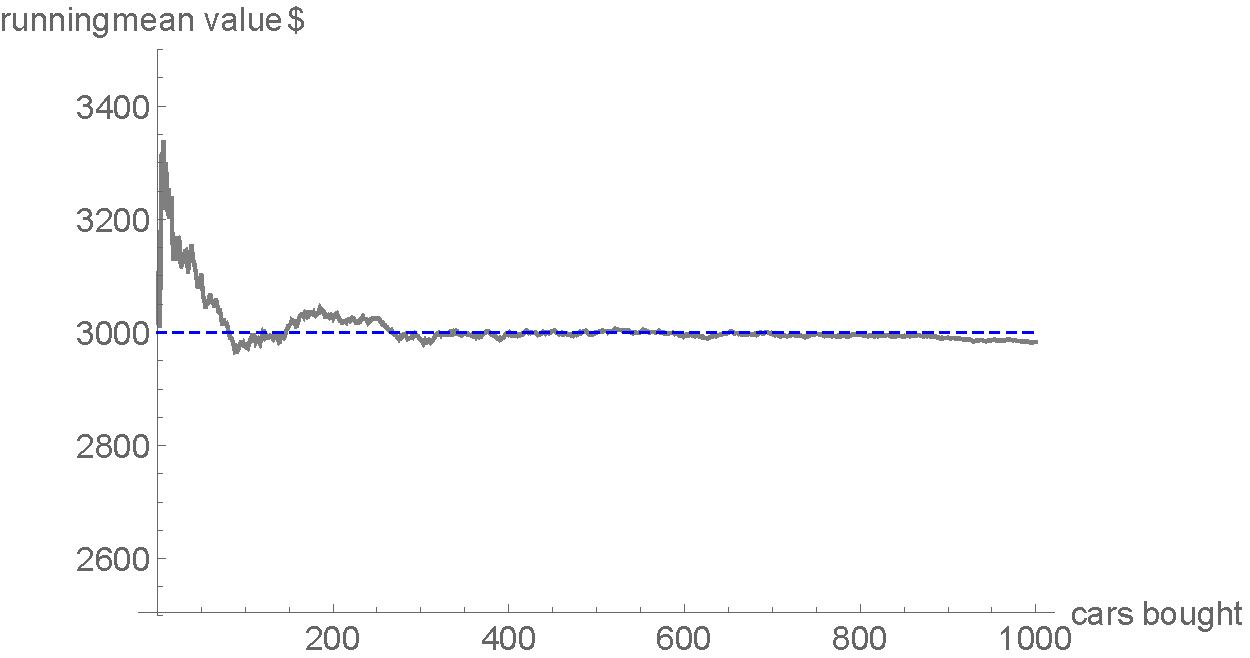
\includegraphics{Intro_meanContinuousLongRun.pdf}}
\caption{Rolling a (computational) die. We show the running average for rolling a fair die a number of times.}\label{fig:Intro_meanContinuousLongRun}
\end{figure}

If you can grasp the process undertaken to produce figures \ref{fig:Intro_meanDiscreteLongRun} and \ref{fig:Intro_meanContinuousLongRun} respectively, then you already understand the basis behind modern computational Bayesian statistics! If you need a bit more explanation of the theory of Bayesian computational, then fear not, we devote an entire Part of the book for this purpose (see Part \ref{part:computationalBayes}).  

Whilst the \textit{mean} of a distribution is a measure of central tendency for a particular distribution, we do not yet have a way of summarising the width of the range of the values of the random variable which are most likely. This motivates the introduction of the concept of a \textit{variance} of a distribution:

\begin{equation}\label{eq:Intro_varianceDistributionExpectations}
var(X) = \mathbb{E}\left(\left[X-\mathbb{E}(X)\right]^2\right)
\end{equation}

To apply this to discrete and continuous distributions respectively, we straightforwardly replace the $\alpha$ on the right-hand side of (\ref{eq:Intro_meanDistributionDiscrete}) and (\ref{eq:Intro_meanDistributionContinuous}) respectively, by $(\alpha-\mathbb{E}(X))^2$ in each case\footnote{This is a specific example of the general rule, that to calculate the mean value of some function $f(X)$, where $X$ is governed by a particular distribution, we do: \begin{equation}
\mathbb{E}(f(X)) = \sum\limits_{All\; \alpha} f(\alpha) Pr(X=\alpha)
\end{equation}
for a discrete distribution, and analogously for the continuous case, but using an integral opposed to a sum.}:

\begin{equation}\label{eq:Intro_varianceDistributionDiscrete}
var(X) = \sum\limits_{All\; \alpha} (\alpha-\mathbb{E}(X))^2 Pr(X=\alpha)
\end{equation}

\begin{equation}\label{eq:Intro_varianceDistributionContinuous}
var(X) = \int\limits_{All\; \alpha} (\alpha-\mathbb{E}(X))^2 p(\alpha)\mathrm{d}\alpha
\end{equation}

If the equations are starting to overwhelm, then fret not, we really only wanted to include them for completeness. What is more important is their significance. Essentially, a \textit{variance} measures the width of the distribution of values obtained around its mean. A wider variance therefore signifies a greater variety of values away from the mean. In figure \ref{fig:Intro_variance} we compare the variability of a fair die, with one heavily biased to take on the values 3 and 4. We see that the variability of the running mean for the loaded die is smaller than that of the fair die, particularly as the number of rolls increases. This is due to the fact that the fair die has a variance of:

\begin{equation}
\begin{align}
var(X) &= \sum\limits_{\alpha=1}^{6} (\alpha-3\tfrac{1}{2})^2\times Pr(X=\alpha)\\
&= \frac{35}{12}
\end{align}
\end{equation}

whereas similar calculations for the loaded die distribution shown in the middle of figure \ref{fig:Intro_variance}, yield a value of $\frac{7}{12}$. To be concrete, the variance of a distribution is an indicator of the long-run average square distance of values away from the mean. 

\begin{figure}
\centering
\scalebox{0.35} 
{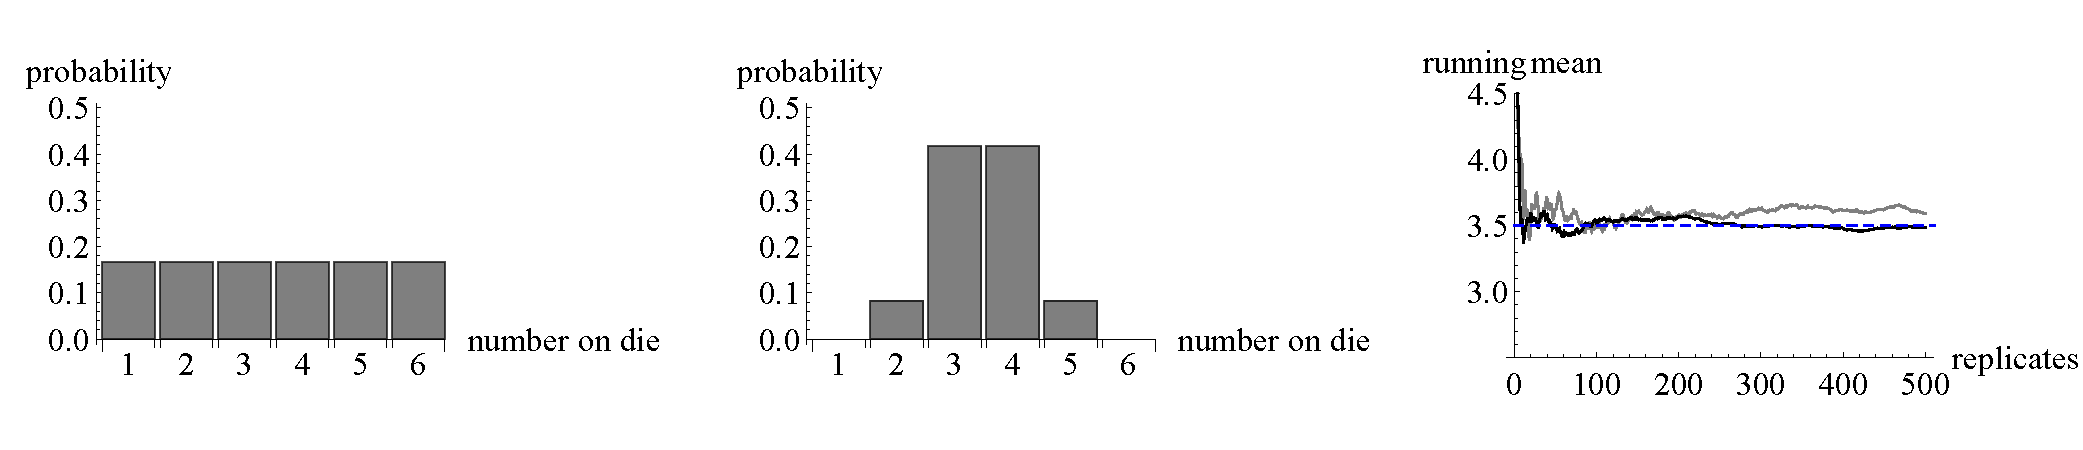
\includegraphics{Intro_variance.pdf}}
\caption{Rolling a (computational) die. We run simulations of a fair die in grey (distribution shown in left graph), and a biased one in black (shown in middle graph), and compare the variability of values around the mean of $\frac{1}{2}$.}\label{fig:Intro_variance}
\end{figure} 

\subsection{Generalising probability distributions to two dimensions}
Life is often more complex than the examples of section \ref{sec:Intro_probabilityDistributions}. Often we are tasked with formulating opinions on a range of different outcomes; each of which may influence or shed light on the other results. We begin by considering the outcome of two measurements, in order to introduce the reader to the mechanics of probability. The great thing is that these rules do not become any more complex when we generalise to higher dimensional problems, meaning that if the reader is comfortable with the following examples, then they should be able to handle the vast majority of probability distribution operations encountered. In Bayesian statistics, being comfortable manipulating probability distributions is essential, since the output of the Bayesian formula - the posterior probability distribution - is used to derive all post-experiment quantities of interest. As such, it is important to devote some time to introduce two examples which we will use to describe and explain the manipulations of 2-dimensional probability distributions in the next few sections.

\subsubsection{Biased coins: a 2-dimensional discrete probability example}\label{sec:Intro_biasedCoinsTwoDimensionalDiscrete}
Imagine that you are given two coins, and you are told that both are biased towards the same particular outcome - heads or tails - although, before flipping them you are unaware as to their inherent prejudice. We are also have an inherent feeling, due to our prior experience with the experimenter, that a bias towards heads is more likely. We use a binary variable to represent the outcome of each coin flip, which takes on the value of 0 if the coin falls tails-up, and 1 if it falls heads-up. We could then represent our beliefs beforehand in the form of a probability distribution shown in table \ref{tab:Intro_coinBiased}.

\begin{table}[htbp]
  \centering
    \begin{tabular}{rrcc}
    \toprule
          &       & \multicolumn{2}{c}{\textbf{Coin A}} \\
    \midrule
          &       & \textbf{0} & \textbf{1} \\
    \multicolumn{1}{c}{\textbf{Coin B}} & \multicolumn{1}{c}{\textbf{0}} & 0.3   & 0.1 \\
    \multicolumn{1}{c}{} & \multicolumn{1}{c}{\textbf{1}} & 0.1   & 0.5 \\
    \bottomrule
    \end{tabular}%
  \caption{The probability distribution for the biased coins example described in section \ref{sec:Intro_biasedCoinsTwoDimensionalDiscrete}. $\{0,1\}$ refers to the coin falling tails- or heads-up respectively.}\label{tab:Intro_coinBiased}
\end{table}

How can we check whether this distribution satisfies the requirements for a valid probability distribution? We simply apply the rules described in section \ref{sec:Intro_validProbabilityDistribution}. Firstly, all the values of the distribution are real and non-negative; satisfying our first requirement. For the second rule rather than summing over the values of one random variable, we now have to sum over the outcome of two:

\begin{equation}\label{eq:Intro_discreteTwoDimensionalCoinSum}
\sum\limits_{X_A=0}^{1}\sum\limits_{X_B=0}^{1} Pr(X_A,X_B) = 0.3 + 0.1 + 0.1 + 0.5 = 1
\end{equation}

In (\ref{eq:Intro_discreteTwoDimensionalCoinSum}), $X_A$ and $X_B$ are random variables\footnote{A function which associates a unique numerical value with each outcome of an experiment. In this case the function gives value 0 if the result is a tails, and 1 if it is heads.} which refer to the outcome of Coin A and Coin B respectively. Notice that since we are now considering a situation with the outcome of two random variables, we are now required to index the probability, $Pr(X_A,X_B)$, by both. Due to the probability now being a function of two variables, we say that the probability distribution is 2-dimensional.

How can we interpret the probability distribution shown in table \ref{tab:Intro_coinBiased}? The probability that both coins show tails (and hence both their random variables take on the value of 0), is simply read off from the top-left entry in the table, meaning $Pr(X_A=0,X_B=0)=0.3$. We ascribe a smaller likelihood to the coins coming up with different outcomes, $Pr(X_A=0,X_B=1)=0.1$ or $Pr(X_A=1,X_B=0)=0.1$, since we believe that the coins are biased in the same direction. We believe that the most likely outcome is that both coins show heads, since we believe that the experimenter is predisposed to this outcome, and hence ascribe the highest probability to this result, with $Pr(X_A,X_B)=0.5$.

\subsection{Foot length and intelligence: a 2-dimensional continuous probability example}
We suppose that we have a sample of individuals, and we measure their foot size, as well as how well they score on an IQ test. Both of these variables can be reasonably be assumed to be continuous, meaning that we are now required to represent our strength of belief, by specifying a probability distribution across a continuum of values (see figure \ref{fig:Intro_footSizeIntelligenceTwoDimensionalExample}). 

\begin{figure}
\centering
\scalebox{0.5} 
{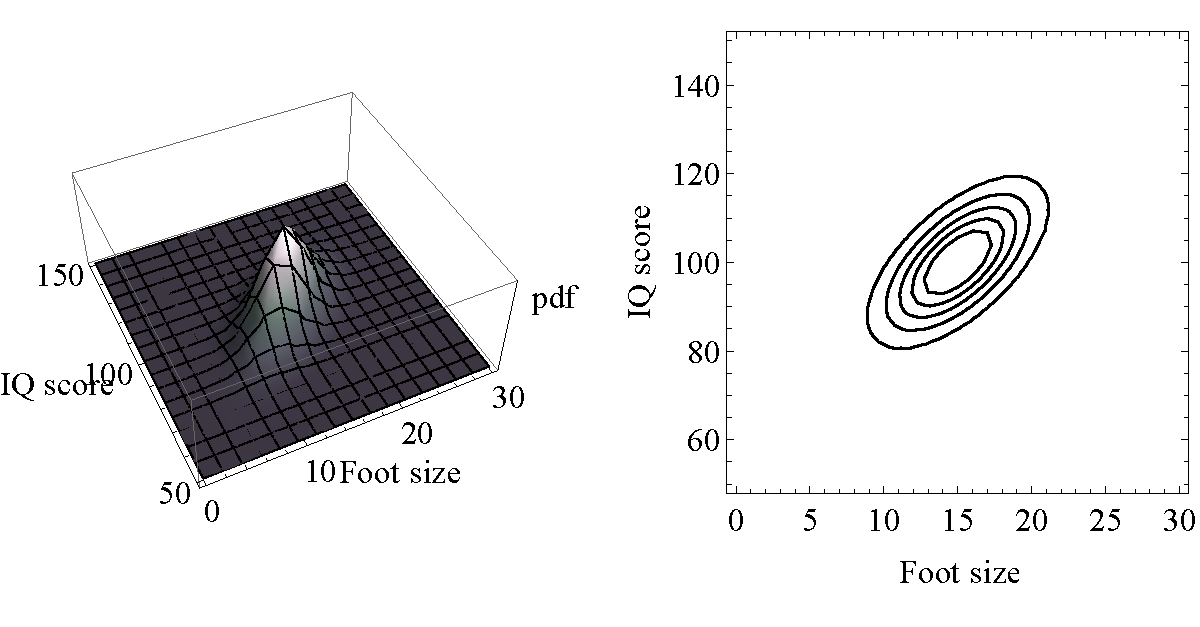
\includegraphics{Intro_footSizeIntelligenceTwoDimensionalExample.pdf}}
\caption{A probability distribution describing the foot size and IQ for an individual within our sample. Left) Represented as a 3-dimensional plot, and Right) Contour lines specify isolines of probability.}\label{fig:Intro_footSizeIntelligenceTwoDimensionalExample}
\end{figure}

We could verify that the distribution shown in figure \ref{fig:Intro_footSizeIntelligenceTwoDimensionalExample} is in fact valid, by showing that the volume underneath the left hand plot is 1, via integration. However, since we don't want to overcomplicate things now, you will have to take our word for it.

Notice that we have chosen to allow there to be a degree of correlation between foot size and IQ. Why might we choose to do this\footnote{Our sample of individuals here is a sample of children of various ages. Age is correlated with shoe size and intelligence.}?

\subsection{Marginal distributions}\label{sec:Intro_marginal}
We may be interested in simplifying the preceding analysis, by stating the distribution of one variable, completely \textit{unconditional} of the other. In our coins example, we might be interested in say, only the value obtained when we flip coin A. Alternatively, we might want to remove the dependence on foot size, in our IQ example, and what remains would then be an \textit{unconditional} probability distribution for IQ.

In order to do this, we essentially need to \textit{average} out the dependence of the other variable. In our coins example, if we are only interested in coin A, we can sum down the column values for coin B, obtaining the \textit{marginal} distribution of coin A, shown at the bottom of table \ref{tab:Intro_coinsMarginal}.


\begin{table}[htbp]
  \centering
    \begin{tabular}{rrccr}
    \toprule
          &       & \multicolumn{2}{c}{\textbf{Coin A}} &  \\
    \midrule
          &       & \textbf{0} & \textbf{1} & \multicolumn{1}{c}{\textbf{$Pr(X_B)$}} \\
    \multicolumn{1}{c}{\textbf{Coin B}} & \multicolumn{1}{c}{\textbf{0}} & 0.3   & 0.1   & \multicolumn{1}{c}{\textbf{0.4}} \\
    \multicolumn{1}{c}{} & \multicolumn{1}{c}{\textbf{1}} & 0.1   & 0.5   & \multicolumn{1}{c}{\textbf{0.6}} \\
          & \multicolumn{1}{c}{\textbf{$Pr(X_A)$}} & \textbf{0.4} & \textbf{0.6} & \multicolumn{1}{c}{} \\
    \bottomrule
    \end{tabular}%
  \caption{The marginal distribution of coins A and B, achieved by summing the values in each column or row respectively.}\label{tab:Intro_coinsMarginal}%
\end{table}%

Hence, we have that the \textit{marginal} probability of coin A coming up 'heads' is 0.6. This value is composed out of the two possible ways in which this \textit{single} event can occur:

\begin{equation}\label{eq:Intro_marginalCoinsExample}
Pr(X_A=1) = Pr(X_A=1,X_B=0) + Pr(X_A=1,X_B=1)
\end{equation}

In (\ref{eq:Intro_marginalCoinsExample}), we see that A can come up 'heads' with B being 'tails', or alternatively A can land on 'heads' with B also on 'heads'.

Thus, in order to calculate the probability of a single event, we simply need to sum across all possible occurrences of it, allowing the other variable to take on its possible values. Mathematically, we can summarise this rule by the following for the case of two discrete random variables:

\begin{equation}\label{eq:Intro_marginalDiscreteProbabilityTwoDimensions}
Pr(A=\alpha) = \sum\limits_{\beta} Pr(A=\alpha,B=\beta)
\end{equation}

In (\ref{eq:Intro_marginalDiscreteProbabilityTwoDimensions}), $\alpha$ and $\beta$ refer to the specific values taken on by the random variables $A$ and $B$. 

We can use (\ref{eq:Intro_marginalDiscreteProbabilityTwoDimensions}) for the coin example to calculate the probability that coin B lands up on 'tails':

\begin{equation}
\begin{align}
Pr(X_B=0) &= \sum\limits_{\alpha=0}^{1} Pr(X_B=0,X_A=\alpha)\\
&= Pr(X_B=0,X_A=0) + Pr(X_B=0,X_A=1)\\
&= 0.3 + 0.1 = 0.4
\end{align}
\end{equation}

For continuous random variables we need the continuous analogue of a sum, an \textit{integral}, in order to calculate the marginal distribution. Intuitively, this is because the other variable is now able to take on an continuum of values:

\begin{equation}\label{eq:Intro_marginalContinuousProbabilityTwoDimensions}
p_A(\alpha) = \int\limits_{All\;\beta} p_{AB}(\alpha,\beta) \mathrm{d}\beta
\end{equation}

In (\ref{eq:Intro_marginalContinuousProbabilityTwoDimensions}), $p_{AB}(\alpha,\beta)$ corresponds to the joint probability distribution of random variables $A$ and $B$ evaluated at $(A=\alpha,B=\beta)$. Similarly, $p_A(\alpha)$ refers to the marginal distribution of random variable A, evaluated at $A=\alpha$. Although it is somewhat of an abuse of notation, for simplicity, from now on we will now write $p_{AB}(\alpha,\beta)$ as $p(A,B)$, and $p_A(\alpha)$ as $p(A)$.

In the foot size/IQ example, we may not be interested in foot size; wanting only the distribution of IQ in our sample. We can obtain this by simply integrating out the dependence on foot size:

\begin{equation}\label{eq:Intro_marginalContinuousProbabilityTwoDimensionsFootExample}
p(IQ) = \int\limits_{0}^{30} p(IQ,FS) \mathrm{d}FS
\end{equation}

The result of carrying out the step in (\ref{eq:Intro_marginalContinuousProbabilityTwoDimensionsFootExample}) is that we are left with the distribution shown on the right of figure \ref{fig:Intro_footSizeIntelligenceMarginal}. We have rotated this graph to emphasise that it is the result of essentially summing\footnote{We really mean integrating, but it is more intuitive to think about this in terms of discrete summing.} across the joint density at each particular value of IQ. 

Another way to think about marginal densities, is imagine that you are walking along the landscape of the joint density. The height of the marginal density is given by the length of the path you have to walk along a particular line of constant IQ. If the path is relatively flat, indicating a low value of joint density, then the corresponding marginal density is low. However, if the path encompasses a large hill, indicating a high value of joint density, then the marginal density will be relatively high.

Add a 3D version of the figure with the contours traced out on the landscape, and leading to the height of the marginals, perhaps with stick figures walking along lines of iso-IQ.

\begin{figure}
\centering
\scalebox{0.5} 
{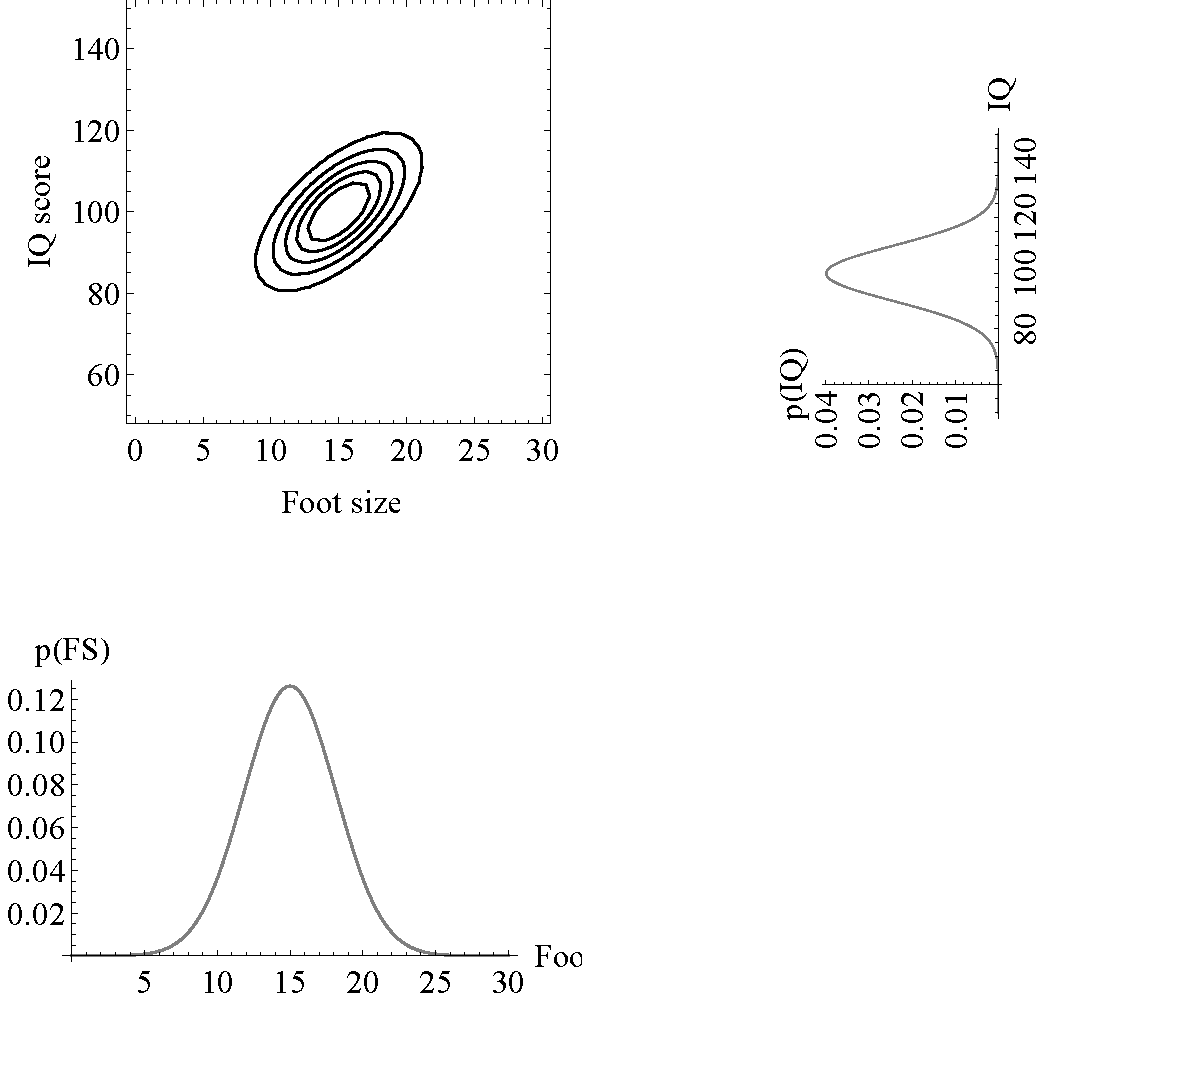
\includegraphics{Intro_footSizeIntelligenceMarginal.pdf}}
\caption{Top-left: the joint density of foot size and intelligence. Right: the marginal density of IQ. Bottom: the marginal density of foot size. \textbf{I want to add a line at a particular value of IQ, and at a particular value of FS, to illustrate the horizontal and vertical summing.}}\label{fig:Intro_footSizeIntelligenceMarginal}
\end{figure}

An alternative way of thinking about marginal distributions is provided by the Venn diagram shown in figure \ref{fig:Intro_Venn}. In a Venn diagram, the area of a particular event indicates its probability, and the rectangular area represents all the events that can possibly happen, and so has an area of 1. We have chosen to specify arbitrary events A and B as sub-areas in the diagram, which overlap indicating a region of joint probability, $p(A,B)$. In this setup it is straightforward to calculate the marginal probability of events A or B; we find the area of the elliptic shapes A or B respectively. Considering event A, when we calculate the area of the entire ellipse, we are implicitly carrying out the sum of the form indicated in (\ref{eq:Intro_marginalDiscreteProbabilityTwoDimensions}):

\begin{equation}\label{eq:Intro_vennMarginals}
p(A) = p(A,B) + p(A,not\; B)
\end{equation}

In (\ref{eq:Intro_vennMarginals}), the terms on the right hand side correspond to the overlap region, and the remaining part of A (where B does not occur) respectively.

\begin{figure}
\centering
\scalebox{0.5} 
{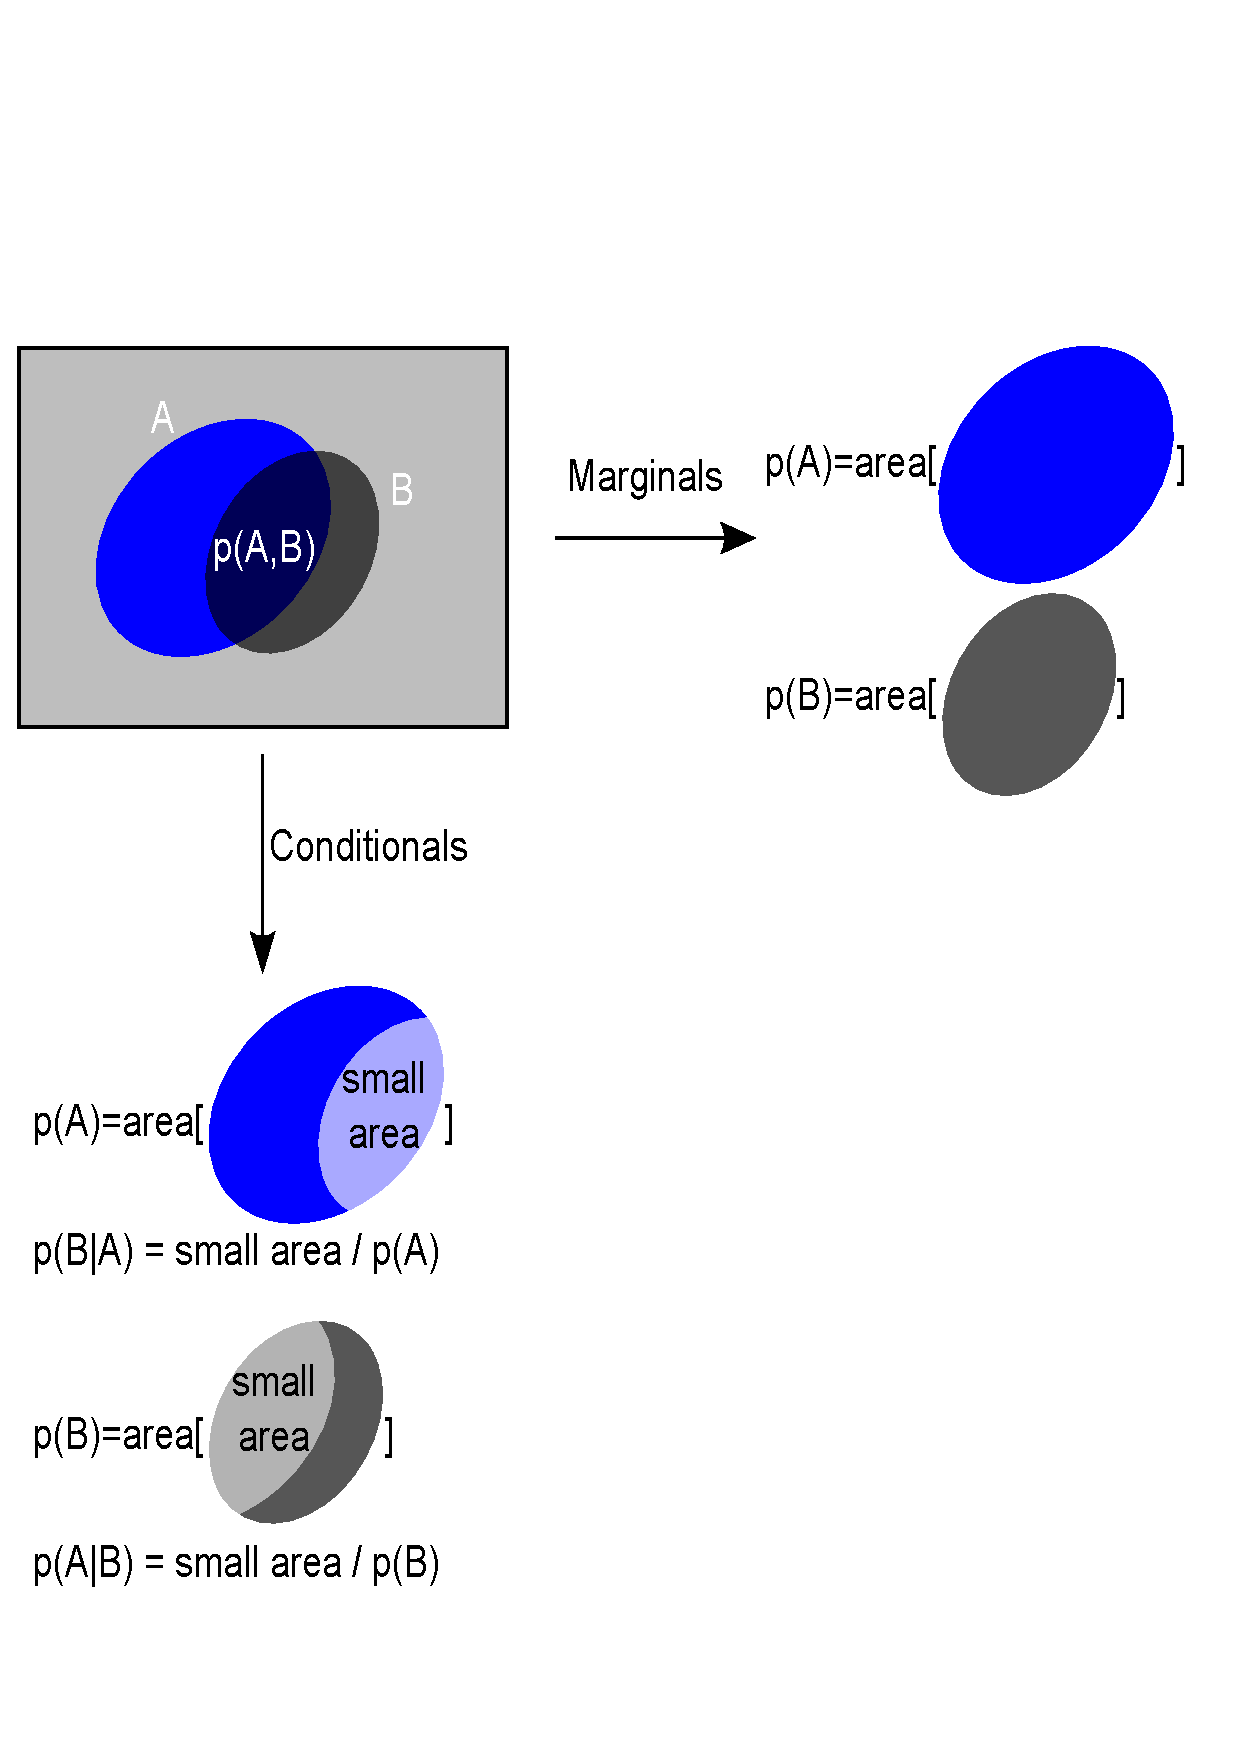
\includegraphics{Intro_Venn.pdf}}
\caption{A Venn diagram showing one way of interpreting marginal and conditional distributions.}}\label{fig:Intro_Venn}
\end{figure}

\subsection{Conditional distributions}
We frequently receive partial information by observing only part of the system in which we are interested. In our coin example, we might flip of one of the coins finding lands heads-up, and on this basis update our probabilities of obtaining heads or tails for the other. Alternatively, in the foot size - IQ example described before, we might measure an individual's shoe size, and then want to obtain the updated probability distribution for IQ scores.

In probability, when we observe one variable, and reformulate the probability distribution for the other variable, we say that we are deriving the \textit{conditional} distribution of the latter. \textit{Conditional} refers to the fact that we are deriving the probability distribution of one variable, \textit{conditional} on the value of the other(s).

In each case, we have reduced some of the uncertainty in the system, by observing one of its characteristics. Hence in the two-dimensional examples described above the conditional distribution is only one-dimensional, because we are only now uncertain about one variable. 

Luckily, there is a simple rule that we can use to obtain the probability of one variable, conditional on the value of the other:

\begin{equation}\label{eq:Intro_conditionalProbability}
p(A|B) = \frac{p(A,B)}{p(B)}
\end{equation}

In (\ref{eq:Intro_conditionalProbability}), $p(A|B)$ refers to the probability of $A$ occurring, given that $B$ has occurred. In the right hand side of (\ref{eq:Intro_conditionalProbability}), $p(B)$ is the \textit{marginal} distribution of B occurring, and $p(A,B)$ is the joint probability of $A$ and $B$ occurring.

We can use (\ref{eq:Intro_conditionalProbability}) for the coins example to calculate the probability that \textit{given} that coin A lands heads-up, what is the probability of coin B also landing heads-up when we flip it?

\begin{equation}\label{eq:Intro_conditionalDiscreteCoins}
\begin{align}
Pr(X_B=1|X_A=1) &= \frac{Pr(X_A=1,X_B=1)}{Pr(X_A=1)}\\
&= \frac{Pr(X_A=1,X_B=1)}{Pr(X_A=1,X_B=0)+Pr(X_A=1,X_B=1)}\\
&= \frac{0.5}{0.1 + 0.5}\\ 
&= \frac{5}{6}
\end{align}
\end{equation}

In (\ref{eq:Intro_conditionalDiscreteCoins}), we have used the rule we discussed earlier for calculating marginal probabilities, shown in (\ref{eq:Intro_marginalDiscreteProbabilityTwoDimensions}), to calculate the denominator, $Pr(X_A=1)$.

Another way to see the workings of this calculation is shown in table \ref{tab:Intro_coinsConditionalDiscrete}. When we uncover that coin A is heads-up, we essentially reduce our solution space to only the central column (highlighted in blue). Therefore we need to renormalise the solution space such that it has a probability of 1, by dividing each of its entries through by its original total of probabilities, 0.6; yielding the conditional probabilities shown in the right hand column of table \ref{tab:Intro_coinsConditionalDiscrete}.

\begin{table}[htbp]
  \centering
    \begin{tabular}{rrccr}
    \toprule
          &       & \multicolumn{2}{c}{\textbf{Coin A}} &  \\
    \midrule
          &       & \textbf{0} & \textbf{1} & \multicolumn{1}{c}{\textbf{$Pr(X_B|X_A=1)$}} \\
    \multicolumn{1}{c}{\textbf{Coin B}} & \multicolumn{1}{c}{\textbf{0}} & 0.3   & {\color{blue}0.1}   & \multicolumn{1}{c}{\textbf{=0.1/0.6 = 1/6}} \\
    \multicolumn{1}{c}{} & \multicolumn{1}{c}{\textbf{1}} & 0.1   & {\color{blue}0.5}   & \multicolumn{1}{c}{\textbf{=0.5/0.6 = 5/6}} \\
          & \multicolumn{1}{c}{\textbf{$Pr(X_A)$}} & \textbf{0.4} & {\color{blue}\textbf{0.6}} & \multicolumn{1}{c}{} \\
    \bottomrule
    \end{tabular}%
\caption{The highlighted region indicates the new solution space, since we know that coin A has landed heads-up.}
\label{tab:Intro_coinsConditionalDiscrete}
\end{table}

The Venn diagram in figure \ref{fig:Intro_Venn} shows another way of interpreting conditional distributions. If we are told that a particular event B occurs, then our event space collapses to only the area specified by B. The conditional probability, $p(A|B)$ is then simply given by the ratio of the area of overlap between A and B to the total area of B. This makes intuitive sense, since this is the only way that event A can occur, given that B has already occurred.

\begin{figure}
\centering
\scalebox{0.5} 
{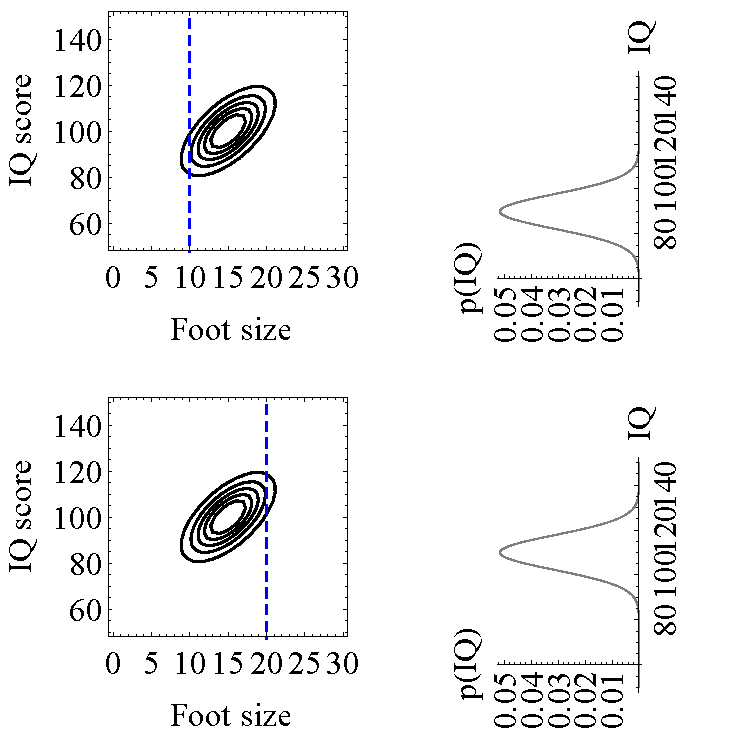
\includegraphics{Intro_footSizeIntelligenceConditional.pdf}}
\caption{The dashed blue lines indicate the new event space in each case. The height walked following these lines is related to the magnitude of the conditional distributions shown on the right.}}\label{fig:Intro_footSizeIntelligenceConditional}
\end{figure}

We can also use (\ref{eq:Intro_conditionalProbability}) to allow us to calculate the conditional distribution of IQ for individuals after we have measured their shoe size. The only difference with the discrete example is that we now have to use an integral to work out the marginal probability for foot size; the denominator of (\ref{eq:Intro_conditionalProbability}). Figure \ref{fig:Intro_footSizeIntelligenceConditional} shows the conditional distributions traced out when we measure an individual's foot size to be 10cm and 20cm respectively. The blue dashed lines show the new event space, since we have lost our uncertainty over foot size in each of the cases. Therefore the heights traversed on the walk along these lines indicate the relative likelihood of different values of IQ. 

\section{Higher dimensional probability densities: no harder than 2-D, just looks it!}
Now that we are equipped with the tools to calculate marginal and conditional distributions in two dimensions, we can use these to work with probability distributions that depend on arbitrary many variables. Although formulae appear more complex, this is really just a result of having to keep track of each individual variable.

For example, suppose that we have a posterior density that is defined in terms of three parameters, $p(\alpha,\beta,\sigma)$. If we wish to determine the posterior solely as a function of $\alpha$ and $\beta$, then we start by defining the parameter vector $\boldsymbol{\theta} = (\alpha,\beta)$, meaning we are left with $p(\boldsymbol{\theta},\sigma)$. Note that all we have done is defined a new composite variable, $\boldsymbol{\theta}$. Now our density is of the '2-dimensional' form shown in (\ref{eq:Intro_marginalContinuousProbabilityTwoDimensions}), and we can apply this relation:\\

\begin{equation}\label{eq:Intro_higherDimensionalMarginal}
\begin{align}
p(\alpha,\beta) &= p(\boldsymbol{\theta})\\
&= \int\limits_{All\; \sigma} p(\boldsymbol{\theta},\sigma)\mathrm{d}\sigma
\end{align}
\end{equation}

If we wish to find the marginal distribution for $\alpha$ \textit{only}, then all we do is integrate the resultant distribution in (\ref{eq:Intro_higherDimensionalMarginal}) with respect to $\beta$.

We can use exactly the same trick to calculate the \textit{conditional} density of $\alpha$ and $\beta$, conditional on observing $\sigma$:

\begin{equation}\label{eq:Intro_higherDimensionsConditional}
\begin{align}
p(\alpha,\beta|\sigma) &= p(\boldsymbol{\theta}|\sigma)\\
&= \frac{p(\boldsymbol{\theta},\sigma)}{p(\sigma)}
\end{align}
\end{equation}

In (\ref{eq:Intro_higherDimensionsConditional}), we have used (\ref{eq:Intro_conditionalProbability}) to arrive at the second line.

Finally, note that combining all parameters of interest into a single parameter vector $\boldsymbol{\theta}$ allows us to calculate \textit{marginal} and \textit{conditional} distributions for probability distributions that depend on an arbitrary number of parameters.

\section{Independence}\label{sec:Intro_independence}
If we think that there is a relationship between two random variables, then we say that they are \textit{dependent}. This does not necessarily mean \textit{causal} dependence, as it is sometimes supposed, in that the behaviour of variable $A$ affects the outcome of variable $B$. What it really means is that the value taken on by $A$ is informative as to the likely value of $B$. 

An example of dependence might be the \textit{colour} and \textit{suit} of a playing card. If we are told that the colour of a playing card is $red$, this means that our other variable \textit{suit} is constrained to be either \textit{hearts} or \textit{diamonds}. In this case, knowing with certainty the value of the first variable, \textit{colour}, helps us to narrow down the list of outcomes of the second variable, \textit{suit} (See figure \ref{fig:Intro_IndependenceCards}).

\begin{figure}
\centering
\scalebox{0.3} 
{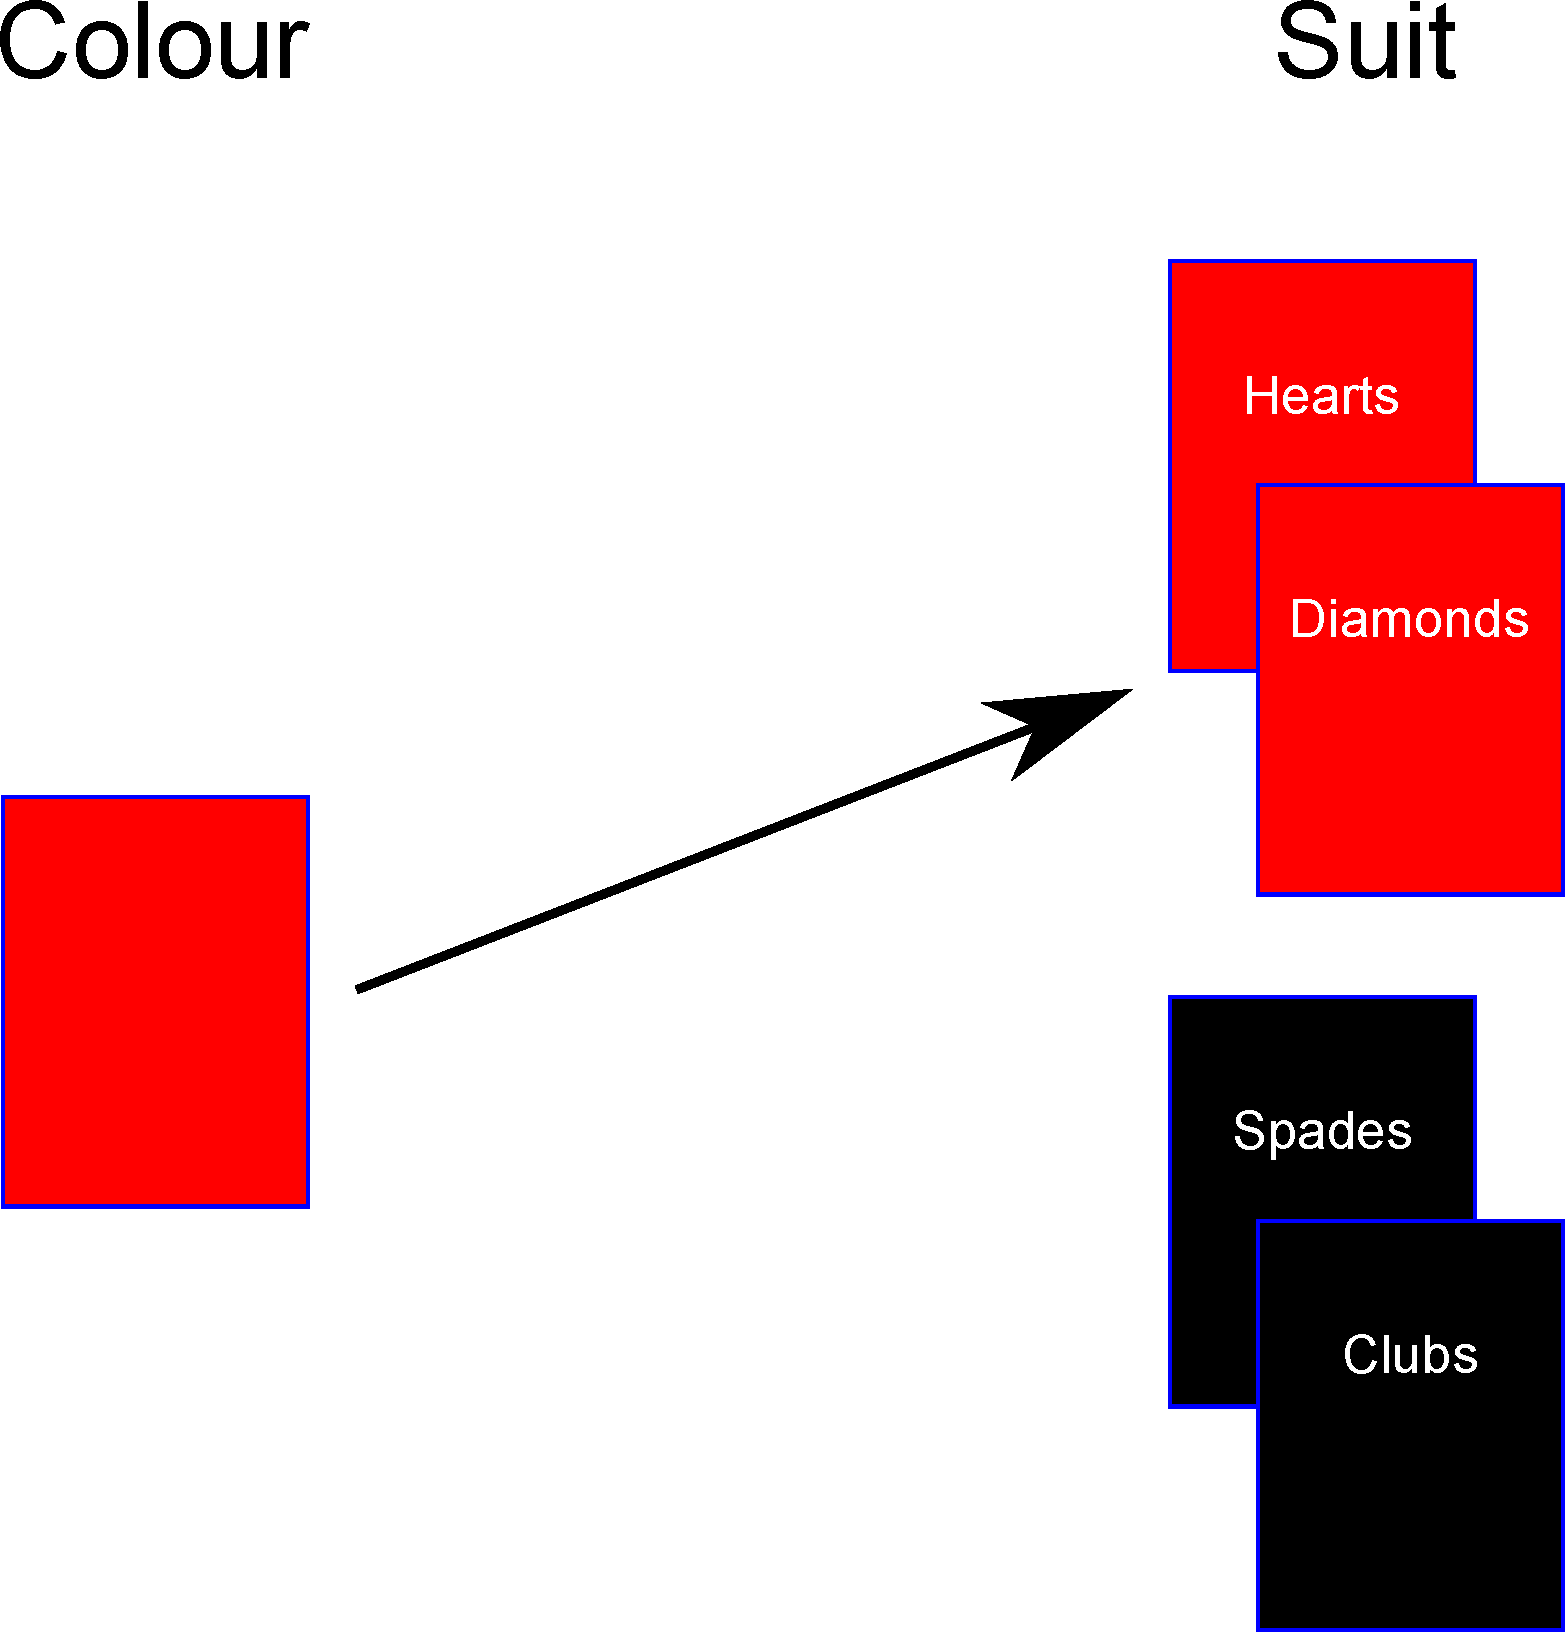
\includegraphics{Intro_IndependenceCards.pdf}}
\caption{Knowledge of the colour of a card provides information about the suit of the card. The colour and suit of a card are \textit{dependent}.}\label{fig:Intro_IndependenceCards}
\end{figure}

Another example of dependent variables, is the weather outside and the suntan of a particular, vein, individual\footnote{Discounting sunbeds.}. If it is sunny, then we assume it is more likely that an individual is tanned. Whereas, if the weather is cloudy, it is less so.

If two variables, $A$ and $B$ are \textit{disjoint}, then if one occurs, then the other cannot. In this case, it is often mistakenly believed that the variables are \textit{independent}, although this is very much not the case (see the left hand panel of figure \ref{fig:Intro_VennIndependence}). In this case, knowledge of variable $A$, provides significant information about variable $B$. If $A$ occurs, then we know for \textit{certain} that $B$ cannot!

\begin{figure}
\centering
\scalebox{0.4} 
{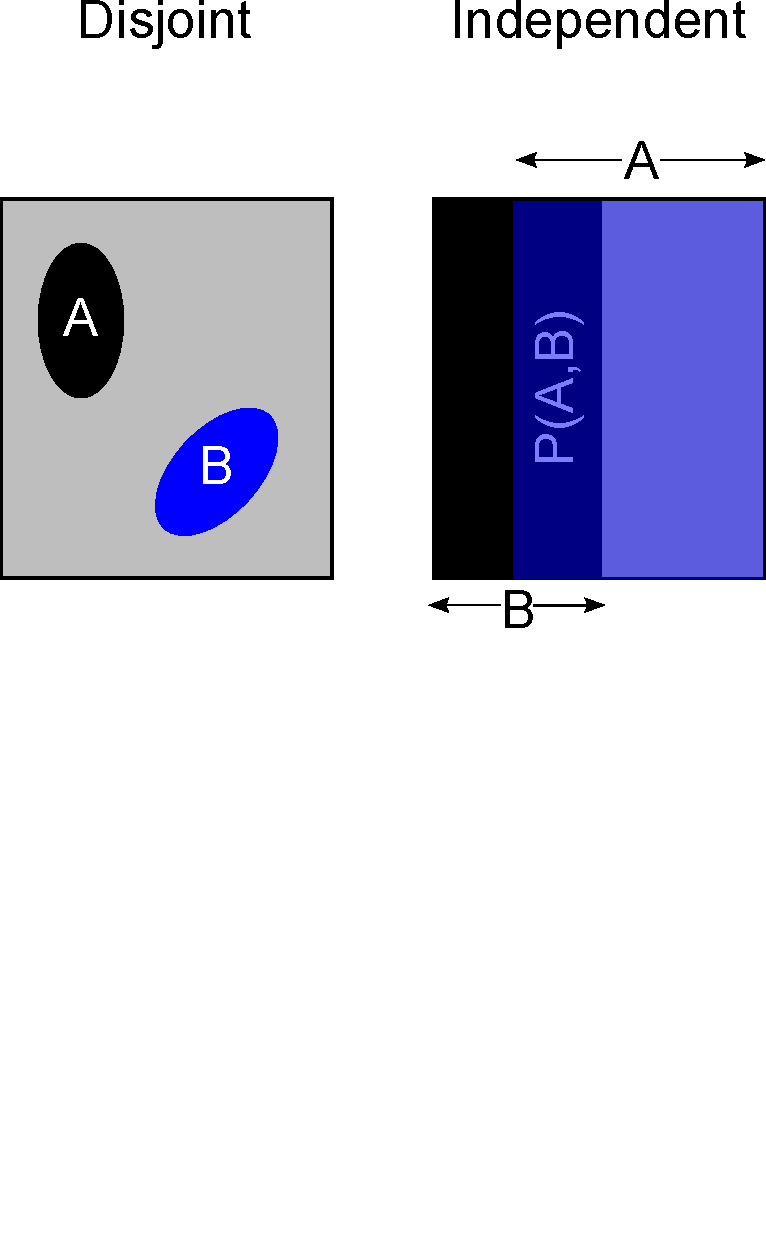
\includegraphics{Intro_VennIndependence.pdf}}
\caption{Venn diagram depictions of left: disjoint, and right: independent, events $A$ and $B$.}\label{fig:Intro_VennIndependence}
\end{figure}

By contrast, if two events are \textit{independent}, then knowledge of $B$ provides no additional information on $A$. Mathematically, this means that the conditional probability of $A$ is equal to the marginal:

\begin{equation}\label{eq:Intro_independentConditionalEqualMarginal}
p(A|B) = p(A)
\end{equation}

Using our conditional probability rule given in (\ref{eq:Intro_conditionalProbability}), we can then use this to rewrite the above as:

\begin{equation}\label{eq:Intro_independentConditionalEqualMarginal1}
\frac{p(A,B)}{p(B)} = p(A)
\end{equation}

In words, the ratio of the area of overlap between $A$ and $B$ to the area of $B$, is the same as the overall probability of $A$ (see the right hand panel of figure \ref{fig:Intro_VennIndependence}). This makes intuitive sense, since uncovering that $B$ has occurred (being in $B$) should result in no change to the probability of $A$ occurring (now $p(A|B)$).

\section{Central Limit Theorems: the most important thing ever}\label{sec:Intro_CLT}


\section{The Bayesian formula}\label{sec:Intro_BayesianFormula}
We first of all rewrite the conditional probability formula (\ref{eq:Intro_conditionalProbability}), regarding the probability of event A occurring, \textit{given} that event B has occurred:

\begin{equation}\label{eq:Intro_conditionalProbabilityAB}
p(A|B) = \frac{p(A,B)}{p(B)}
\end{equation}

However, we could also swap A and B around leading to the following for the probability of B \textit{given} that A has already occurred:

\begin{equation}\label{eq:Intro_conditionalProbabilityBA}
p(B|A) = \frac{p(B,A)}{p(A)}
\end{equation}

We however reason from the Venn diagram in figure \ref{fig:Intro_Venn}, that the overlap region of $p(A,B)$ really translated means, the probability of A \textit{and} B occurring. This means that this is exactly the same as the reverse; the probability of B \textit{and} A coinciding, $p(B,A)$. We can therefore rearrange (\ref{eq:Intro_conditionalProbabilityBA}) for this joint probability:

\begin{equation}\label{eq:Intro_jointConditionalProbability}
p(A,B) = p(B|A)\times p(A)
\end{equation}

We can use (\ref{eq:Intro_jointConditionalProbability}) to break down the probability of both A and B occurring into two steps. Firstly, for this to happen we require that A \textit{must} happen, with its corresponding probability $p(A)$. Then for both to occur, we straightforwardly require the probability of B occurring, \textit{given} that A has already occurred, which is given by $p(B|A)$. This reasoning provides a little intuition as to the workings of the conditional probability law that we wrote down in (\ref{eq:Intro_conditionalProbability}).

We can finally substitute (\ref{eq:Intro_jointConditionalProbability}) into the numerator of the fraction in (\ref{eq:Intro_conditionalProbabilityAB}), to yield the famous Bayesian formula!

\begin{equation}\label{eq:Intro_BayesianFormula}
p(A|B) = \frac{p(B|A)\times p(A)}{p(B)}
\end{equation}

The Bayesian formula importantly tells us how to correctly convert from $p(B|A)$ to its inverse $p(A|B)$, which is central to Bayesian statistics.

\subsection{The intuition behind the formula}
If we multiply both sides of (\ref{eq:Intro_BayesianFormula}) by $p(B)$, we arrive at the following alternative statement of Bayes' rule:

\begin{equation}\label{eq:Intro_BayesianIntuition}
p(A|B)\times p(B) = p(B|A)\times p(A) \;\;\;[= p(A,B)]
\end{equation}

In (\ref{eq:Intro_BayesianIntuition}), we have added the final part in square parentheses due to the reasoning of section \ref{sec:Intro_BayesianFormula}, that both sides are equivalent to the joint probability of A and B.

What the relation (\ref{eq:Intro_BayesianIntuition}) tells us however, is that there are two ways of arriving at this joint probability (see figure \ref{fig:Intro_BayesianIntuition}). The first way is given by the left hand side, and is due to B occurring, with probability $p(B)$, followed by A \textit{given} that B has occurred, with probability $p(A|B)$. An exactly equivalent way route to both A and B occurring is given by the right hand side of the leftmost equals sign. Here we require that A occurs first, with probability $p(A)$, followed by B \textit{given} that A has occurred, with probability $p(B|A)$.

\begin{figure}
\centering
\scalebox{0.4} 
{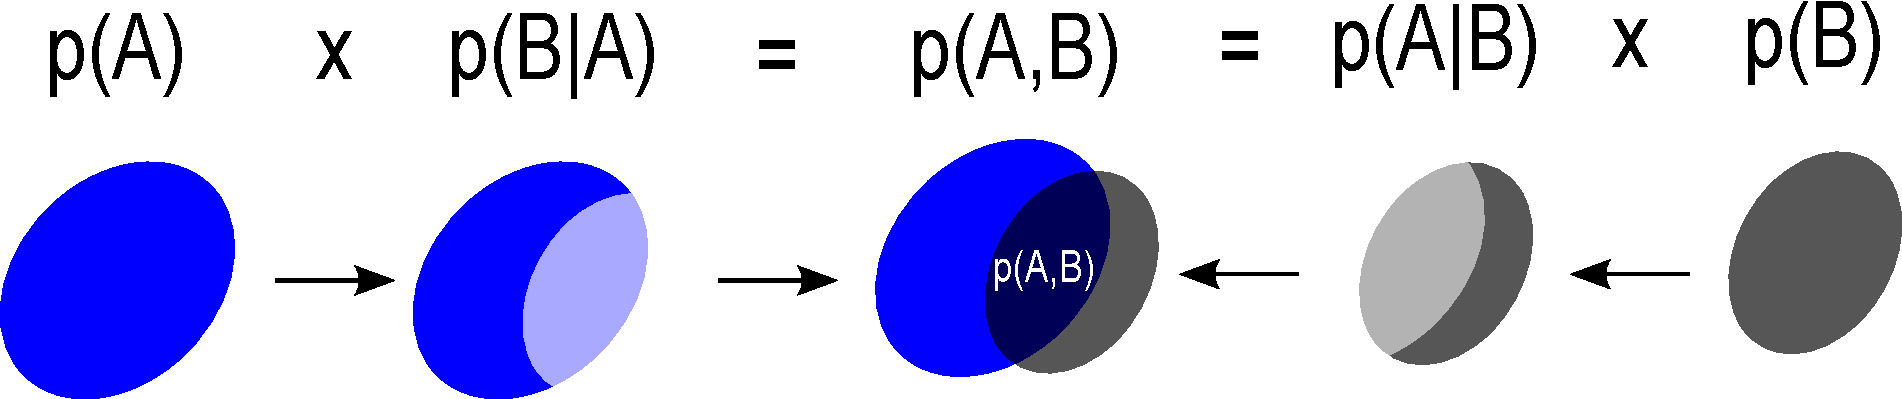
\includegraphics{Intro_BayesianIntuition.pdf}}
\caption{The two ways of arriving at the joint probability $p(A,B)$; providing some intuition behind Bayes' rule.}\label{fig:Intro_BayesianIntuition}
\end{figure}

\section{The Bayesian inference process from the Bayesian formula}
In Bayesian statistics we aim to use probability distributions to describe all components of our system. Our starting point is Bayes' rule:

\begin{equation}\label{eq:Intro_BayesianFormula1}
p(A|B) = \frac{p(B|A)\times p(A)}{p(B)}
\end{equation}

In statistics we typically are looking to estimate a number of parameters, which we will from now on call $\theta$, which represent a component of a statistical model which we build to represent a particular phenomena. These parameters - whether they are merely abstractions, or are real quantities - are defined in terms of a particular population of interest. However, we typically do not have data for the whole population, and hence we must make do with a sample of \textit{data}. 

In Bayesian statistics, we want to derive our beliefs for parameters \textit{given} that we have obtained a particular sample of data. Being Bayesians, we would like to represent these beliefs via a probability distribution, which we write as $p(\theta|data)$. However, we can use (\ref{eq:Intro_BayesianFormula1}), (if we associate $A$ with $\theta$, and $B$ with the \textit{data}) to write:

\begin{equation}\label{eq:Intro_BayesianInferenceFormula}
p(\theta|data) = \frac{p(data|\theta)\times p(\theta)}{p(data)}
\end{equation}

Although we have straightforwardly made two substitutions to arrive at (\ref{eq:Intro_BayesianInferenceFormula}) from (\ref{eq:Intro_BayesianFormula1}), what have we gained by doing so? Also, what exactly do the terms on the right hand side actually mean?

\subsection{Likelihoods}\label{sec:Intro_likelihoods}
Starting with the numerator on the right hand side of (\ref{eq:Intro_BayesianFormula1}), we come across the term $p(data|\theta)$, which we call the \textit{likelihood}. This tells us the probability of generating the particular sample of \textit{data}, if the parameters in our statistical model were equal to $\theta$. When we write down a statistical model, we can generally calculate the probability of particular outcomes, so this is easily obtained. Imagine that we have a coin that we believe to be fair. By \textit{fair}, we typically mean that the probability of the coin falling 'heads-up' is $\theta=\frac{1}{2}$. If we flip the coin twice, we might suppose that it is reasonable to model the outcomes as independent (see section \ref{sec:Intro_independence}), and hence we can calculate the probabilities of the four possible outcomes, by multiplying the probabilities of the individual outcomes together:

\begin{equation}
\begin{align}
p(HH) &= p(H)\times p(H) = \frac{1}{2} \times \frac{1}{2} = \frac{1}{4}\\
p(HT) &= p(H)\times p(T) = \frac{1}{2} \times \frac{1}{2} = \frac{1}{4}\\
p(TH) &= p(T)\times p(H) = \frac{1}{2} \times \frac{1}{2} = \frac{1}{4}\\
p(TT) &= p(H)\times p(H) = \frac{1}{2} \times \frac{1}{2} = \frac{1}{4}\\
\end{align}
\end{equation}

Hence, we obtained a \textit{sample} of two heads, we could write down the corresponding likelihood, $p(HH|\theta=\frac{1}{2})=\frac{1}{4}$.

Do not worry if you do not fully understand this concept, as we will be devoting an entire chapter to likelihoods in chapter \ref{chap:Likelihoods}.

\subsection{Priors}\label{sec:Intro_priors}
The next term in the numerator of the right hand side, $p(\theta)$ is the most controversial\footnote{Although this controversy is unwarranted, as we explain in section \ref{sec:Intro_implicitExplicitSubjectivity}.} part of the Bayesian formula, which we call the \textit{prior} distribution of $\theta$. It is a probability distribution which represents our pre-data beliefs as to the likely values of the parameters in our model, $\theta$. This appears at first to be slightly counter-intuitive, particularly if you are used to the world of classical statistics, which does not require us to state our preferences \textit{explicitly}\footnote{Although, we always do \textit{implicitly}, as we explain in section \ref{sec:Intro_implicitExplicitSubjectivity}.}. Continuing the coin example, we might assume that we do not know whether the coin is fair or biased beforehand, so we might think that all possible values of $\theta\in[0,1]$ - which represents the probability of the coin falling 'heads-up' are equally likely. We might represent these beliefs by a continuous uniform probability density on this interval (see the left-hand graph of figure \ref{fig:Intro_priors}). Normally however, we might think that coins are manufactured such that the weight distribution is fairly symmetrical on either face; meaning that we expect that the majority of coins are reasonably fair. These latter beliefs of unbiasedness might be fairly well represented by the right-hand graph of figure \ref{fig:Intro_priors}.

\begin{figure}
\centering
\scalebox{0.6} 
{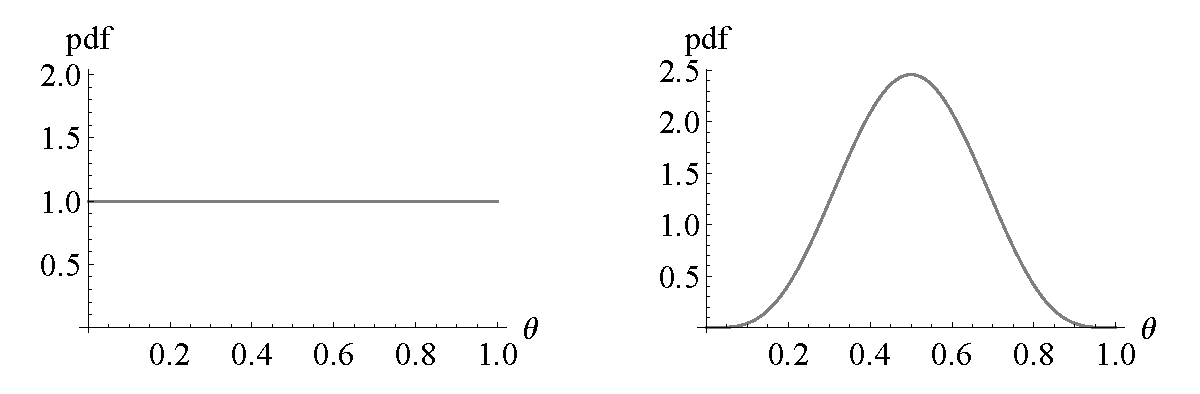
\includegraphics{Intro_priors.pdf}}
\caption{Left: All values of a the bias of a coin are equally likely. Right: It is believed that the coin is most likely fair.}\label{fig:Intro_priors}
\end{figure}

The concept of \textit{priors} will be covered in detail in chapter \ref{chap:Prior}.

\subsection{The denominator}
The final term on the right hand side, on the denominator is $p(data)$. This represents the probability of obtaining our particular sample of data, if we assume a particular model and prior. We will mostly postpone further discussion of this term until chapter \ref{chap:denominator}, when we understand better the significance of \textit{likelihoods} and \textit{priors} respectively. However, note that this denominator is actually a marginal probability density (see section \ref{sec:Intro_marginal}), which can be obtained from summing/integrating the joint density $p(\theta,data)$ with respect to the parameter(s) of the model.

The concept of \textit{the denominator} will be covered in detail in chapter \ref{chap:denominator}.

\subsection{Posteriors: the goal of Bayesian inference}
The posterior probability distribution $p(\theta|data)$ is often the main goal of Bayesian inference. For example, in the coin example described before, we might want to derive a probability distribution representing our post-experimental beliefs of the inherent bias, $\theta$, of a coin, \textit{given} that we flipped it 10 times, and it came up 'heads' 7 times. If we use (\ref{eq:Intro_BayesianInferenceFormula}), assuming the likelihood model specified in \ref{sec:Intro_likelihoods} and the flat uniform prior shown in figure \ref{fig:Intro_priors}, then we would end up with a posterior distribution shown in figure \ref{fig:Intro_posterior}. Notice that the peak of the distribution occurs at $\theta=0.7$, which corresponds exactly with the percentage of 'heads' seen in the experiment\footnote{Note that if we chose a non-uniform prior, this peak would most likely shift.}. 

\begin{figure}
\centering
\scalebox{0.6} 
{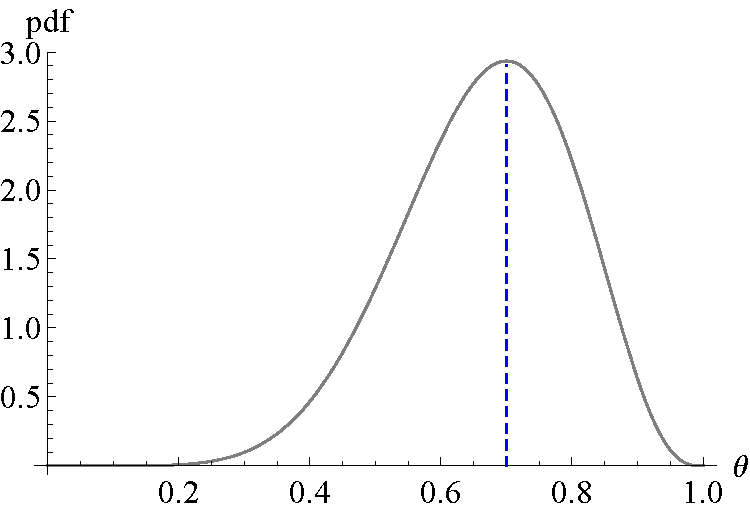
\includegraphics{Intro_posterior.pdf}}
\caption{The posterior distribution for, $\theta$, the bias of a coin when flipped, assuming a flat uniform prior and Bernoulli likelihood. We assume that 7/10 times the coin came up 'heads'.}\label{fig:Intro_posterior}
\end{figure}

The posterior distribution summaries our uncertainty in parameter values. If the distribution is more peaked, then this emphasises that there is a greater degree of certainty with a particular value for a parameter. This increased certainty over a parameter value is frequently obtained by collecting more data. In figure \ref{fig:Intro_posteriorPeaked}, we compare the posterior distribution for the previous case of 7/10 times a coin appearing 'heads' up, with a new, larger, sample where 70/100 times the same coin comes up 'heads'. In both cases the same ratio of 'heads' to 'tails' appeared, resulting in the same peak value of $\theta=0.7$. However, in the latter case, since we have more evidence to support our claim, we end up with greater certainty over the parameter value after the experiment.

\begin{figure}
\centering
\scalebox{0.6} 
{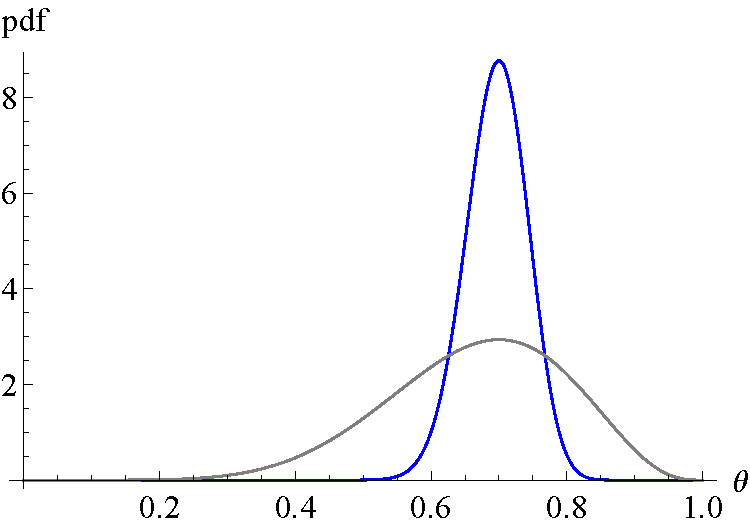
\includegraphics{Intro_posteriorPeaked.pdf}}
\caption{Posterior distributions for, $\theta$, the bias of a coin when flipped, assuming a flat uniform prior and Bernoulli likelihood. The grey line assumes that 7/10 times the coin came up 'heads'. The blue line is for the case where 70/100 times the coin came up 'heads'.}\label{fig:Intro_posteriorPeaked}
\end{figure}

The posterior distribution is also used as a starting point for prediction of future outcomes of an experiment, as well as for model testing. However, we will leave discussion of these until later chapters.

\section{Implicit vs Explicit subjectivity}\label{sec:Intro_implicitExplicitSubjectivity}
One of the major arguments levied against Bayesian statistics is that it is by its nature \textit{subjective}, due to its dependence on the analyst specifying their pre-experimental beliefs through \textit{priors}. This experimenter prejudice towards certain outcomes is said to bias the results away from the types of fair, objective outcomes resultant from a classical analysis. 

We argue that \textit{all} analyses involve a degree of subjectivity, which is \textit{implicitly} assumed. In a classical analysis, the statistician typically states a model for probability which depends on a range of assumptions, which are generally justified. This process of justification is indicative of the subjective nature of the assumptions on which most analyses rest. For example, the choice to use a simple \textit{linear regression model} in many applied classical analyses assumes that the response of a dependent variable is linear in the model's parameters, and frequently the independent variables. This choice of model architecture is generally arbitrary, and used mostly to simplify the analysis. 

In science, there is a tendency amongst scientists to use data to suit one's needs, although this practice should really be discouraged (see ref for 'why most analyses are wrong'). This choice as to which data points to include is subjective, and will remain independent of the type of analysis applied. 

A further source of subjectivity is in the way in which models are checked and tested. In analyses, both classical and Bayesian, there is a need to exercise (subjective) judgement in suggesting a methodology which will be used in this process. We would argue that a Bayesian analysis allows greater flexibility, and suitable methodologies for these processes, since the prior- and posterior- predictive distributions are straightforwardly manipulated to suit most situations. A Bayesian methodology also allows different models to be compared in a logically-coherent manner, whilst classical analysis relies on fairly arbitrary criteria \footnote{$\bar{R^2}$, AIC and BIC are examples} to do so.

In contrast to the examples of \textit{subjectivity} which we have mentioned above, Bayesian \textit{priors} are \textit{explicitly} stated. This makes this part of the analysis openly available to the reader, allowing it to be as thoroughly interrogated and debated, as any part of an argument. This transparent nature of Bayesian statistics has lead many to suggest that it is \textit{honest}; whilst classical analyses hide behind a fake veil of \textit{objectivity}, Bayesian equivalents explicitly acknowledge the subjective nature of all analyses.

Furthermore, the more data that is collected, the less impact the prior exerts on posterior distributions. In any case, if slight modification to priors results in a different conclusion being reached, it is the job of the researcher to report this sensitivity. In fact, in contrast to classical analyses, a Bayesian analysis allows for a range of models/priors to be stated, which can then be used to test the sensitivity of conclusions to any subjective assumptions made.

\section{What are the tangible (non-academic) benefits of Bayesian statistics?}
In Bayesian textbooks much discourse is devoted to advocating the academic reasons for choosing to use a Bayesian analysis over classical approaches. However, often authors neglect to promote the more tangible, everyday benefits of the former. Here, we list the following \textit{real} benefits of a Bayesian approach:

\begin{itemize}
\item \textbf{Simple and intuitive model testing and comparison}. The prior- and posterior-predictive distributions allow for in-depth testing of any particular aspect of a model, by comparing it with the same aspects from the data collected. The Bayesian approach also provides a logical framework in which to compare different models.
\item \textbf{Straightforward interpretation of results.} In classical analyses, the \textit{confidence interval} is often taken to be a measure of uncertainty for a particular parameter. As we shall see in section \ref{sec:Posterior_classicalConfidenceInterval}, this is not the case, and interpretation of this concept is not straightforward. By contrast Bayesian \textit{credible intervals}, can be taken to be a measure of uncertainty in a parameter, as they are obtained directly from probability distributions.
\item \textbf{Full model flexibility}. Modern Bayesian analyses use computational simulation in order to carry out analyses. Whilst this might appear excessive when compared to classical approaches, an additional benefit is the straightforward extension to almost arbitrarily complex models when using Bayesian approaches. This means that Bayesian models can be extended to encompass any complexity of data process. This is in contrast to classical approaches, where the intrinsic difficulty of analysis scales with the complexity of the model chosen.
\item \textbf{The best predictions.} Leading figures both inside and outside of academia use Bayesian approaches for prediction. An example being Nate Silver's correct prediction of the 2008 US Presidential election results \cite{silver2012signal}.
\end{itemize}

\section{Why don't more people use Bayesian statistics?}
Many are discouraged from using Bayesian approaches to analysis due to its supposed \textit{difficulty}, and dependence on mathematics. However, we would argue that this is, in part, a weakness of the existent literature on the subject, which this book looks to address. It also highlights how many books on classical statistics sweep their inherent complexity and assumptions under the carpet, resulting in texts which are easy to digest; meaning that for many the path of least resistance is to forge ahead with classical tools. 

By its dependence on the logic of probability, this means on first glances, Bayesian statistics appears more mathematically-complex. However, what is often lost in introductory texts on Bayesian theory, is the intuitive explanations behind the mathematical formulae. In this text instead, we shift the emphasis towards the latter; choosing to focus on graphical and illustrative explanations rather than getting lost in the details of the mathematics, which to be honest, is not necessary for much of modern Bayesian analysis. We hope that by doing so, we shall lose fewer casualties to mathematical complexity, and redress the imbalance between classical and Bayesian analysis applications.

Again, on first appearances, the concept of the \textit{prior} no doubt leads many to 'abandon ship' early on the path to understanding better Bayesian methodologies. However, as discussed in section \ref{sec:Intro_priors}, and will be covered in detail in chapter \ref{chap:Prior} which is fully-devoted to this subject, we hope to banish this particular thorn in the side of would-be Bayesian statisticians.

The reliance on computing, in particular simulation, is also seen to add to the complexity of Bayesian approaches. Whilst, this is true, we argue that the modern algorithms used for simulation are straightforward to understand, and with modern software, easy to implement. Furthermore, the added complexity of simulation methods is more than compensated by the straightforward extension of Bayesian models to handle arbitrarily complex situations. Like most things worth learning, there is a slight learning curve to become acquainted with the languages used to write modern Bayesian simulations. However, we hope to make this curve sufficiently shallow by incremental introduction of elements used in these computational applications.

\chapter{The posterior - the goal of Bayesian inference}\label{chap:posterior}
\section{Chapter Mission statement}
At the end of this chapter the reader will understand the central importance, and use of the posterior probability distribution in Bayesian statistics.

Insert a graphic with the likelihood part of Bayes' formula circled, as in the equation shown below for the part highlighted in blue.

\begin{equation}
{\color{blue}P(\theta|data)} = \frac{P(data|\theta)\times P(\theta)}{P(data)}
\end{equation}\label{eq:Posterior_BayesHighlighted}

\section{Chapter goals}
Calculating the posterior distribution for a model's parameters is the focus of undertaking Bayesian analysis. This \textit{probability distribution} which results from the application of Bayes' rule (see \ref{eq:Posterior_BayesHighlighted}) can be used to infer the effects of given variables, to forecast, compare different models of phenomena, as well as test its own foundations! In order to do justice to the multitude of uses of the posterior distribution, it is necessary that the reader is familiar with the basics of probability distributions explained in section . After this we will be able to appreciate how the posterior distribution of Bayes' formula can be put to its many uses. 

\section{Expressing uncertainty in a parameter through the posterior probability distribution}
Unlike looking out the window, getting exam results, or playing a hand at blackjack, we frequently in inference never learn the \textit{true}\footnote{Whether a true value for a parameter actually exists we leave until section \ref{sec:Posterior_parametersExist}.} state of nature. The uncertainty here is both in the future and \textit{present}; the latter meaning we are unable to perfectly measure the state of the world today, and hence cannot hope to perfectly know the former.

\subsection{Do parameters actually exist and have a point value? Bayesian vs classical standpoints}\label{sec:Posterior_parametersExist}
\subsection{Failings of the classical confidence interval}\label{sec:Posterior_classicalConfidenceInterval}
The asymptotic reliance of classical confidence intervals.
\subsection{The HDI as a better alternative}
\subsection{The central posterior interval}

\section{Prediction using a posterior distribution}
\subsection{Before experiment, using prior}
\subsection{After experiment, using posterior}

\section{Model comparison using the posterior}
\section{Model testing through the posterior}

\chapter{Likelihoods}\label{chap:Likelihoods}
\begin{quotation}
The world is everything that is the case. \textbf{Wittgenstein}
\end{quotation}

\section{Chapter Mission statement}
At the end of this chapter a reader will know how to go about selecting a likelihood which is appropriate to a given situation. Further the reader will understand the basis behind maximum likelihood estimation.

Insert a graphic with the likelihood part of Bayes' formula circled, as in the equation shown below for the part highlighted in blue.

\begin{equation}
P(\theta|data) = \frac{{\color{blue}P(data|\theta)}\times P(\theta)}{P(data)}
\end{equation}\label{eq:Likelihood_BayesHighlighted}

\section{Chapter goals}
The starting point of the right hand side of the Bayesian formula is the likelihood function. This chapter will explain what is meant by a likelihood function, and why it is incorrect to view it as a probability in Bayesian analyses. The choice over which likelihood to use for a given situation is often difficult; especially to those unfamiliar with statistics. This chapter will provide practical guidance on likelihood choice, describing a framework that can be used to select a model in a systematic way. As an important stepping stone to Bayesian estimation, this chapter will also explain how classical maximum likelihood estimation works. 

\section{What is a likelihood?}
In all statistical inference, we use an idealised, simplified, model to try to mimic relationships between real variables of interest. This model is then used to test hypotheses about the nature of the relationships between these variables. In Bayesian statistics the evidence for a particular hypothesis is summarised in posterior probability distributions. Bayes' magic rule tells us how we can compute this posterior probability distribution for a given parameter within a model, $\theta$:

\begin{equation}
P(\theta|data) = \frac{P(data|\theta)\times P(\theta)}{P(data)}
\end{equation}\label{eq:Likelihood_Bayes}

The first step to understanding this formula (so that we can ultimately use it!) is to understand what is meant by the numerator term, $P(data|\theta)$, which Bayesians call a Likelihood! Firstly, it's important to say that what we really mean by the numerator is:

\begin{equation}
P(data|\theta) = Probability(data|\theta,Model \; Choice)
\end{equation}\label{eq:Likelihood_simple}

What (\ref{eq:Likelihood_simple}) means is, what is the probability that we would have obtained the 'data', given (this is represented by the $|$ symbol) a particular value of $\theta$ and a particular choice of model. In other words, if our statistical model were true, and the value of the model's parameter were $\theta$, (\ref{eq:Likelihood_simple}) tells us the probability that we would have obtained our data. 

But what does this mean in simple, everyday language? Imagine that we flip a \textit{fair} coin. The most simple statistical model for coin flipping we can pick is to disregard the angle it was thrown at, as well as its height above the surface, along with any other details, and just pick the probability of the coin coming heads to be $\theta=\frac{1}{2}$. Furthermore, if a coin is thrown twice, we might choose to model the situation by assuming that the throwing technique is sufficiently similar between the two throws such that we can model each throw as independently having a probability of $\frac{1}{2}$. It's important to note that it is an assumption to forget about the throwing angle, as well as height of throw for each throw, and this forms part of our model of the situation. 

We can use our simple model\footnote{Albeit in practicality, this is a pretty reasonable representation of the situation for most purposes.} to calculate the probability that we obtain two heads in a row:

\begin{equation}
\begin{align}
P(HH|\theta,Model) &= P(H|\theta,Model)\times P(H|\theta,Model)\\
&= \theta \times \theta = \theta^2\\ 
&= \frac{1}{2}\times \frac{1}{2} = \frac{1}{4}
\end{align}
\end{equation}\label{eq:Likelihood_fairCoin}

The last row of (\ref{eq:Likelihood_fairCoin}) is obtained by assuming the probability of a head, $theta=\frac{1}{2}$. If we continue to use this \textit{same} value of $theta$, we can calculate the corresponding probabilities for all outcomes of throwing the coin twice. The most heads that can show up is 2, and the least being zero (if both flips come up tails). Figure \ref{fig:Likelihood_fairCoin} displays the probabilities for this model of the situation. The most likely number of heads to occur is 1, since this can occur in two different ways - either the first coin comes up heads, and the second is tails, or vice versa - whereas the other possibilities (all heads, or no heads) can each only occur in one way. However, the important thing to note about figure \ref{fig:Likelihood_fairCoin} isn't the individual probabilities, it is that it is a \textit{valid} probability distribution, because:

\begin{itemize}
\item The individual event probabilities are all non-negative.
\item The sum of the individual probabilities is 1.
\end{itemize}

So it appears when we assume a particular value of $theta$, and vary the data (in this case the number of heads obtained), the collection of resultant probabilities form a probability distribution. So, why do Bayesians call $P(data|\theta)$ a 'likelihood', and eschew the name 'probability'?

\begin{figure}
\centering
\scalebox{0.5} 
{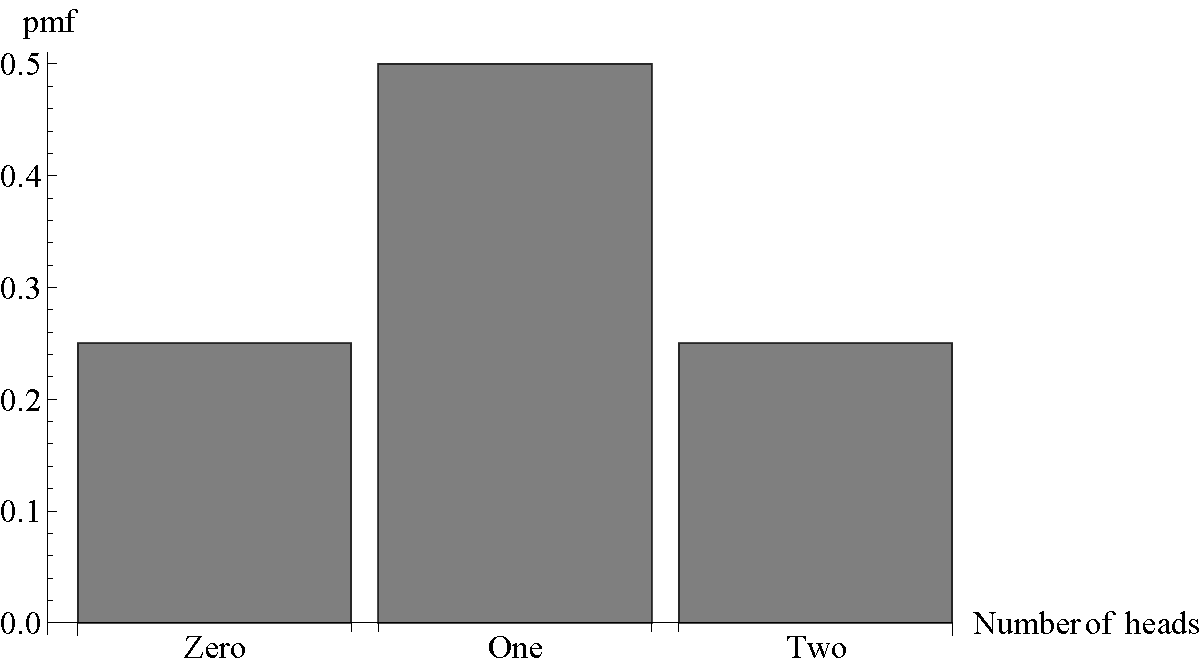
\includegraphics{Likelihood_fairCoin.pdf}}
\caption{The probabilities of all possible numbers of heads for a fair coin.}\label{fig:Likelihood_fairCoin}
\end{figure}

\section{Why use 'likelihood' rather than 'probability'?}
When we hold the parameters of our model fixed, as when we held the probability of an individual throw turning up heads, $\theta=\frac{1}{2}$, we've reasoned that the first term of the numerator of Bayes' rule in (\ref{eq:Likelihood_Bayes}) is a probability. So why don't we just keep calling it that, instead of renaming it a 'likelihood'? 

The reason is that in Bayesian inference, we \textit{don't} keep the parameters of our model fixed! In Bayesian analysis, it is the \textit{data} that is fixed, the parameters that vary. This is because a posterior distribution shows the probability a parameter in a model lies in a particular range, assuming that we have obtained our particular data sample. For the case of a coin, where we don't know the probability of a head beforehand, what we hope to get out is a probability distribution of the kind shown in figure \ref{fig:Likelihood_posteriorExample}, where the x-axis is the value of $\theta$. In order to get $P(\theta|data)$ however, we must calculate $P(data|\theta)$ from the numerator of Bayes' rule in (\ref{eq:Likelihood_Bayes}) for each \textit{possible} value of $theta$. If we assume we obtained two heads, and vary $\theta$ between 0 and 1, we can obtain the likelihood shown in figure \ref{fig:Likelihood_coinLikelihood}. On first glances it appears that \ref{fig:Likelihood_coinLikelihood} could be a probability distribution, but first looks can be deceiving. 

\begin{figure}
\centering
\scalebox{0.5} 
{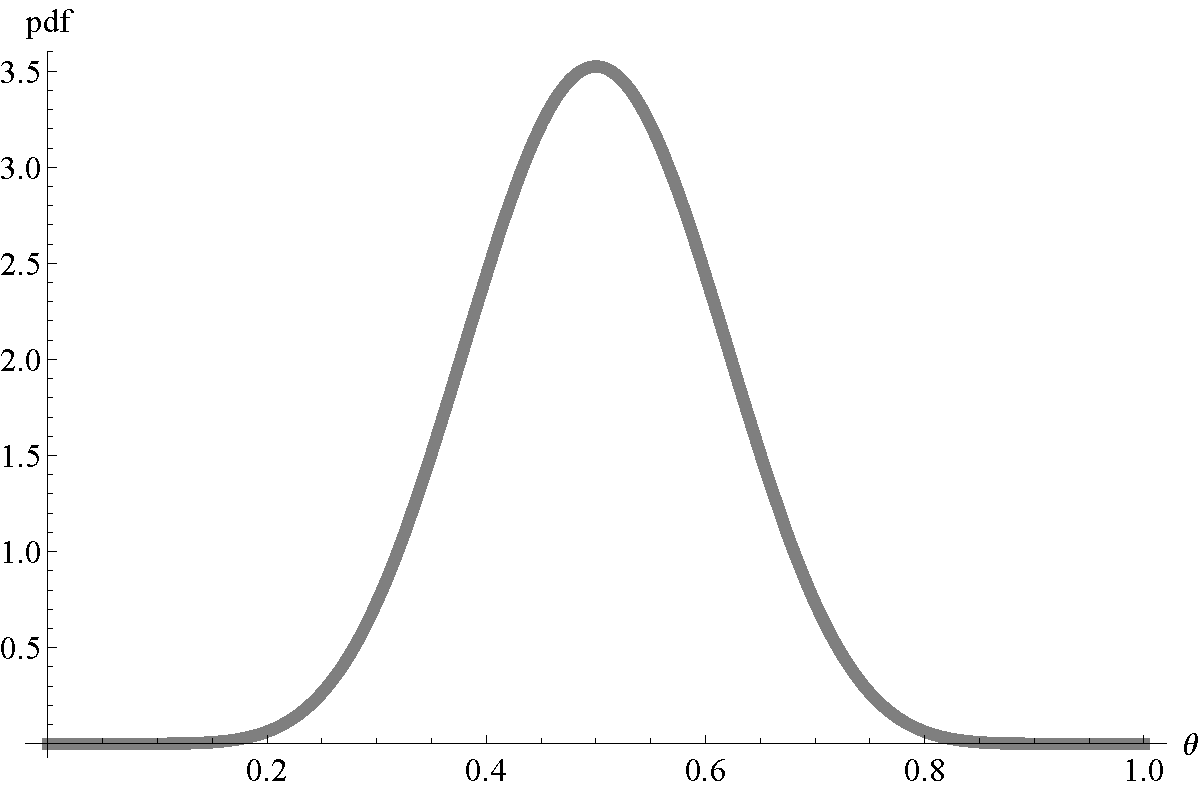
\includegraphics{Likelihood_posteriorExample.pdf}}
\caption{An example posterior distribution for the probability of obtaining a heads in a coin toss.}\label{fig:Likelihood_posteriorExample}
\end{figure}

\begin{figure}
\centering
\scalebox{0.5} 
{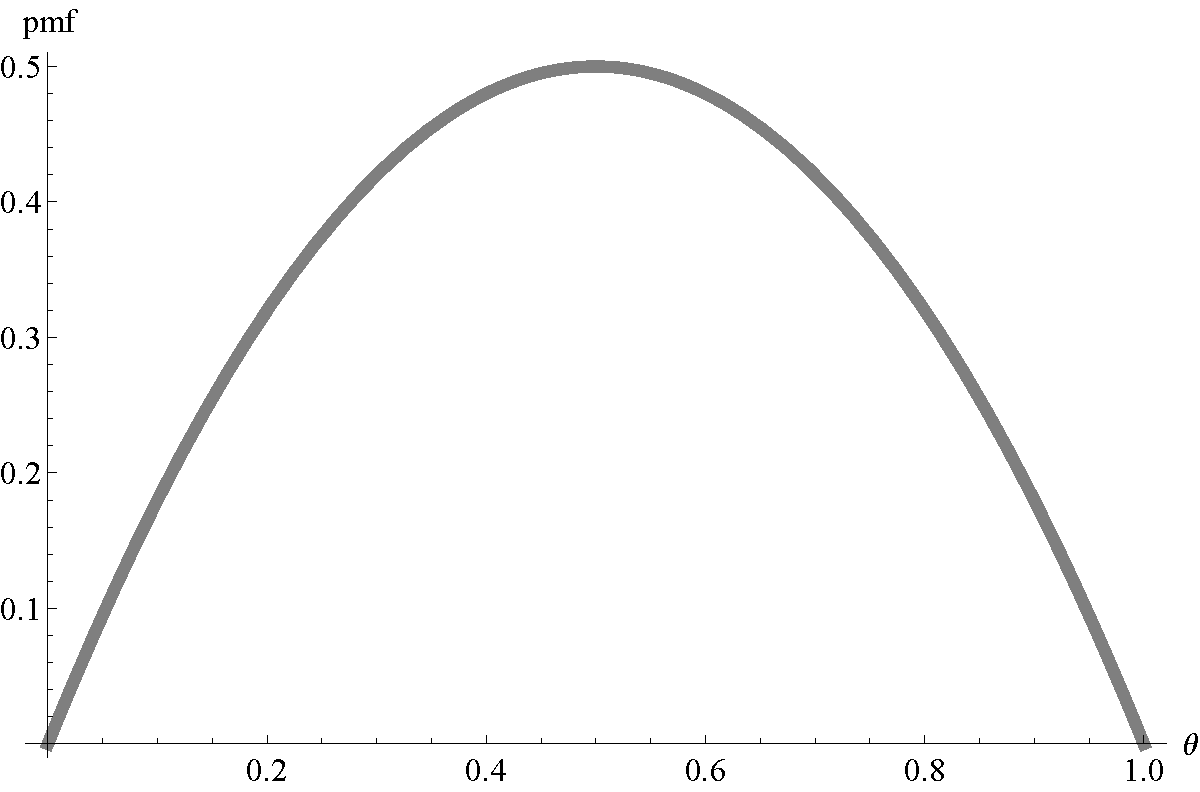
\includegraphics{Likelihood_coinLikelihood.pdf}}
\caption{The likelihood function for obtaining a single head from two throws. The area under the curve is $\frac{1}{3}$.}\label{fig:Likelihood_coinLikelihood}
\end{figure}

Checking off our necessary components of a probability distribution, we first note that all the values of the distribution in figure \ref{fig:Likelihood_coinLikelihood} are non-negative; which is what we require. However, if we look at the area underneath the curve in figure \ref{fig:Likelihood_coinLikelihood}, we find that it does not integrate to 1. Thus we have a violation of the second condition for a valid probability distribution. Hence, when we vary $\theta$ we find that, $P(data|\theta)$ is not a valid probability distribution! We thus introduce the term 'likelihood' to represent $P(data|\theta)$ when we vary the parameter, $\theta$. Often the following notation is used to emphasise that likelihood is a function of the parameter $\theta$ with the data held fixed:

\begin{equation}\label{eq:Likelihood_notation}
\mathcal{L}(\theta|data) = P(data|\theta)
\end{equation}

However, in this book, we will persist with the original notation as this is most typical in the literature, under the implicit assumption that when we vary the parameters in question, the term is not strictly a probability.

To provide further justification for this argument, consider the following (albeit contrived) example. Suppose that, we throw a coin twice, and we are told beforehand that the probability of obtaining a head on a particular throw is one of six discrete values: $\theta\in\{0.0,0.2,0.4,0.6,0.8,1.0\}$. We can then use our model to calculate the probability of obtaining a number of heads, $X$:

\begin{align}\label{eq:Likelihood_OneHead}
P(X = 0|\theta)& = P(TT|\theta) = P(T|\theta)\times P(T|\theta) = (1-\theta)^2\\
P(X = 1|\theta)& = P(HT|\theta) + P(TH|\theta) = 2\times P(T|\theta)\times P(H|\theta) = 2\theta(1-\theta)\\\label{eq:Likelihood_TwoHead}
P(X = 2|\theta)& = P(HH|\theta) = P(H|\theta)\times P(H|\theta) = \theta^2
\end{align}

In (\ref{eq:Likelihood_OneHead}), the probability is simply given by the product of the probabilities of not obtaining a head on the first throw, $(1-\theta)$, by the probability of not obtaining a head in the second\footnote{Since we have assumed a model whereby the results of the first and second throws are independent, conditional on $\theta$. In other words, all the similarity between the two throws is captured in the parameter $\theta$.}, which is also $(1-\theta)$. The factor of two arises in (\ref{eq:Likelihood_TwoHead}) since there are two ways of getting one head: \{HT,TH\}.

We can represent the corresponding values of likelihood/probability as is shown in table \ref{tab:Likeihood_BayesBox}. In this form we can see the impact of varying the data (moving along each row), and contrast it with the effect of varying $\theta$ (moving down each column). Note that if we hold the parameter fixed - regardless of this initial choice of $\theta$ - and move along each row summing the entries, we find that the values sum to 1; meaning that this is a valid probability distribution. By contrast, when we hold the number of heads fixed, and vary the parameter $\theta$, moving down each column, summing the entries, we find that the values do not sum to 1. Hence, when we vary $\theta$, we are not dealing with a proper probability distribution, meriting the use of the term 'likelihood'.

In Bayesian inference, we always vary the parameter, and implicitly hold the data fixed. Thus, from a Bayesian perspective it is important to use the term \textit{likelihood} to indicate that we recognise we are not dealing with a probability distribution.


\begin{table}[htbp]
  \centering
  
    \begin{tabular}{ccccc}
    \multicolumn{5}{c}{\textbf{Number of heads}} \\
    \midrule
    \textbf{$\theta$} & \multicolumn{1}{c}{\textbf{0}} & \multicolumn{1}{c}{\textbf{1}} & \multicolumn{1}{c}{\textbf{2}} &  \multicolumn{1}{c}{\textbf{Total}} \\
    \hline
    \textbf{0.0} & \multicolumn{1}{c}{1.00} & \multicolumn{1}{c}{0.00} & \multicolumn{1}{c}{0.00} & \multicolumn{1}{c}{\textbf{1.00}} \\
    \textbf{0.2} & \multicolumn{1}{c}{0.64} & \multicolumn{1}{c}{0.32} & \multicolumn{1}{c}{0.04} & \multicolumn{1}{c}{\textbf{1.00}} \\
    \textbf{0.4} & \multicolumn{1}{c}{0.36} & \multicolumn{1}{c}{0.48} & \multicolumn{1}{c}{0.16} & \multicolumn{1}{c}{\textbf{1.00}} \\
    \textbf{0.6} & \multicolumn{1}{c}{0.16} & \multicolumn{1}{c}{0.48} & \multicolumn{1}{c}{0.36} & \multicolumn{1}{c}{\textbf{1.00}} \\
    \textbf{0.8} & \multicolumn{1}{c}{0.04} & \multicolumn{1}{c}{0.32} & \multicolumn{1}{c}{0.64} & \multicolumn{1}{c}{\textbf{1.00}} \\
    \textbf{1.0} & \multicolumn{1}{c}{0.00} & \multicolumn{1}{c}{0.00} & \multicolumn{1}{c}{1.00} & \multicolumn{1}{c}{\textbf{1.00}} \\
    \bottomrule
    \textbf{Total} & \multicolumn{1}{c}{\textbf{1.20}} & \multicolumn{1}{c}{\textbf{1.60}} & \multicolumn{1}{c}{\textbf{2.20}} &  \\
    
    \end{tabular}%
  %
  \caption{The values of likelihood for the case of tossing a coin twice, where the probability of heads is constrained to take on a discrete value: \{0.0,0.2,0.4,0.6,0.8,1.0\}.}\label{tab:Likeihood_BayesBox}
\end{table}

\section{What are models and why do we need them?}
All models are wrong. They are idealised representations of reality resultant from making assumptions, which if reasonable, may emulate some of the behaviour of a system of interest. Joshua Epstein in an article titled, 'Why model?' emphasises that we perennially build \textit{implicit} mental models for various phenomena \cite{epstein2008model}. Before we go to bed at night we set our alarms for the next morning on the basis of a model. We imagine an idealised - model - morning when it takes us 15 minutes to wake up as a result of an alarm. We use this model to predict how long it will take us to rise from bed, shower, and get changed into clothes in sufficient time to get to work. Whenever we go to the Doctor, they use an internalised biological model of the human body to advise on the best course of treatment for a particular ailment. Whenever we hear expert opinions on TV about the outcome of an upcoming election, the pundits are using mental models of society to explain the results of current polls, as well as make forecasts. As is the case with all models, some of these models are better than others. Hopefully, the models a Doctor uses to prescribe medicine are subject to less error than the opinions of pundits seen on TV! 

Epstein goes on to emphasise that the question, 'Why model?' really means why should we build an \textit{explicit} - written down - model of phenomena? The point being that \textit{implicit} models are by their very nature, opaque, and not subject to the sort of interrogation and calibration that can be obtained by writing the model on paper. 

We can also ask more narrowly, what are we hoping to gain by building an \textit{explicit} model of a situation? Epstein suggests the following motivations:

\begin{itemize}
\item Prediction
\item Explanation
\item Guide data collection
\item Discover new questions
\item Bound outcomes to plausible ranges
\item Illuminate uncertainties
\item Challenge the robustness of prevailing theory through perturbations
\item Reveal the apparently simple (complex) to be complex (simple) 
\end{itemize}

There are of course other reasons to build models, but we believe that this list is a reasonable starting point. However, we should not think of this list as static. Whenever we build a model, whether it is statistical, biological or sociological, we should ask, 'What are we hoping to gain by building this model, and how can I judge its success?'. Only when we have a grasp on the answers to these basic questions should we proceed to model building.

\section{How to choose an appropriate likelihood?}\label{sec:chooseLikelihood}
Bayesians are acutely aware that their models are wrong. At best the abstraction from reality allows us to explain some aspect of real behaviour; at worst they can be very misleading. Before we use a model for prediction, we require that it can explain some reasonable proportion of the system's behaviour for the past and present. With this in mind we introduce the following model selection framework:

\begin{enumerate}
\item Write down the real life behaviour/data patterns that the model should be capable of explaining.
\item Write down the assumptions that it is believed are reasonable in order to achieve the above point.
\item Search the literature for models which utilise these assumptions; extracting only the relevant components.
\item Test your model's ability to explain said behaviour/data patterns. If unsuccessful go back to the second step and re-evaluate the appropriateness of your assumptions.
\end{enumerate}

Whilst this methodology is useful for building a statistical model in general, it is more applicable for use with a full Bayesian model, resulting in a posterior distribution. In which case how do we go about specifying a likelihood for a given situation? To answer this we will start with going through a simple example.

\subsection{A likelihood model for an individual's disease status}\label{sec:Likelihood_individualDisease}
Suppose we work for the NHS and we want to build a statistical model to explain the prevalence of a certain disease within a sample, which can then be used to make inferences about the population incidence. Also, (unrealistically) let's imagine that we start off with a sample of only one person, for whom we have no prior information. Let the disease status of that individual be denoted by the variable $X$ which takes on the following binary outcome values dependent on the disease status the individual:

\begin{equation}
X =
\begin{cases}
O & , No\; disease \\
1 & , Positive \; diagnosis
\end{cases}
\end{equation}

The goal of our model is to output a probability that this individual has the disease. We might assume that a fraction $\theta$ of the population has the disease, and that this individual has come from that population. For each possible outcome, we can use this simple model to calculate the probability of each outcome:

\begin{align}\label{eq:Likelihood_SimpleModel1}
P(X = 0|\theta)& = (1-\theta)\\
P(X = 1|\theta)& = \theta\label{eq:Likelihood_SimpleModel2}
\end{align}

However, we would like to write down a single rule which yields (\ref{eq:Likelihood_SimpleModel1}) or (\ref{eq:Likelihood_SimpleModel2}) respectively, dependent on whether $X=0$ or $X=1$. This can be achieved with the following:

\begin{equation}\label{eq:Likelihood_bernoulli}
P(X=\alpha|\theta) = \theta^\alpha(1-\theta)^{1-\alpha}
\end{equation}

Note that in (\ref{eq:Likelihood_bernoulli}) that $\alpha\in\{0,1\}$ refers to the numeric value taken by the variable $X$. The function (\ref{eq:Likelihood_bernoulli}) is known as a \textit{Bernoulli} probability density.

Although this rule for calculating a probability of a particular disease status, $\alpha$, looks complex, we see that it reduces to (\ref{eq:Likelihood_SimpleModel1}) and (\ref{eq:Likelihood_SimpleModel2}) if the individual is disease -negative/-positive respectively:

\begin{align}\label{eq:Likelihood_SimpleModel3}
P(X = 0|\theta)& = \theta^0(1-\theta)^1 = (1-\theta)\\
P(X = 1|\theta)& = \theta^1(1-\theta)^0 = \theta\label{eq:Likelihood_SimpleModel4}
\end{align}

When we hold the datum $X$ fixed, and vary $\theta$ (\ref{eq:Likelihood_bernoulli}) represents a likelihood. However, figure \ref{fig:Likelihood_bernoulli} shows that for a fixed value of $theta$ the sum (here we mean the vertical sum) of the two probability densities is always equal to 1; demonstrating that in this case (\ref{eq:Likelihood_bernoulli}) is a valid probability density. Notice also in figure \ref{fig:Likelihood_bernoulli} that the sum of probability density is defined continuously on $\{0,1\}$, whereas the sum of likelihoods is discrete.

\begin{figure}
\centering
\scalebox{0.75} 
{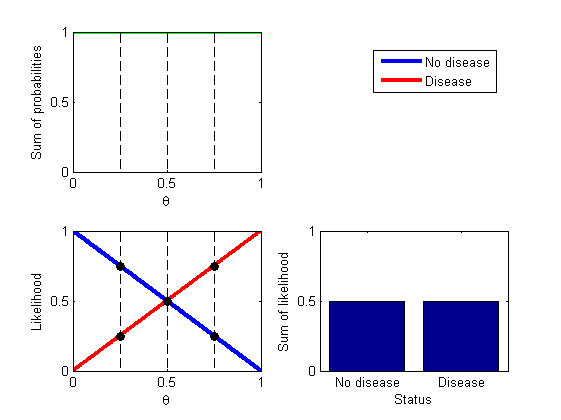
\includegraphics{likelihood_bernoulli.png}}
\caption{The likelihood function as theta varies for the case of the two possible data. The sum of likelihoods is found by the area under each line, whereas the sum of probabilities is a discrete sum.}\label{fig:Likelihood_bernoulli}
\end{figure}

\subsection{A likelihood model for disease prevalence of a group}\label{sec:Likelihood_diseaseGroup}
Now we imagine that instead of this solitary individual, we have a group of $N$ individuals. What we would like to do is to calculate the develop a model which will tell us the probability of obtaining $Z$ disease cases within our sample. We would also like to be able to use our model to predict the most likely number of individuals who have the disease in a sample, for a given value of the parameters\footnote{We are starting off by assuming that we know the parameters. Later in this chapter we will obtain a point estimate of the parameters using \textit{Maximum likelihood} estimation.}. 

In order to write down a model we first need to make some simplifying assumptions. We might assume that one individual's disease status tells us nothing about the probability of another individual in the sample having the disease\footnote{Other than, if the disease prevalence were unknown, through our ability to estimate overall disease prevalence from their individual statuses}. This would not be a reasonable assumption if the disease were contagious, and if the individuals in the sample came from the same neighbourhood or household. It also would not be a good assumption if (as is often the case with volunteer-dependent studies) the individuals who volunteered for the experiment, self-selected on the basis of some common pre-existing ailment/underlying-factor. If an advert for participants reads, 'Psychological experiment on sleep disorders: participants wanted', we might suspect that there would be an over-presence of insomniacs than is found in the population as a whole. This first assumption is that which in statistical language we call 'independence'. We also suppose that all individuals in our sample come from the same population - the one we are trying to draw conclusions about. If we knew beforehand that some individuals came from different populations, with significantly different prevalence rates, then we might abandon this assumption. Combining these two assumptions we say in statistical language that our data sample is \textit{independent} and \textit{identically-distributed}.

With our two assumptions in hand, we can begin to formulate a model for the probability of obtaining $Z$ disease-positive individuals out of a total of $N$ individuals. We start by considering each person's disease status individually, meaning we can reuse (\ref{eq:Likelihood_bernoulli}):

\begin{equation}\label{eq:Likelihood_bernoulli1}
P(X=\alpha|\theta) = \theta^\alpha(1-\theta)^{1-\alpha}
\end{equation}

Note that in (\ref{eq:Likelihood_bernoulli1}) the $\alpha\in\{0,1\}$ refers to a particular numeric value taken by the variable $X$. The assumption of \textit{independence} means that we can get the overall probability by multiplying together the individual probabilities (include reference back to discussion of probabilities). In words, we obtain the probability that the first person has disease status $X_1$ \textit{and} the second person has status $X_2$:

\begin{equation}\label{eq:Likelihood_bernoulli2}
\begin{align}
P(X_1=\alpha_1,X_2=\alpha_2|\theta_1,\theta_2) &= P(X_1=\alpha_1|\theta_1)\;\times \;P(X_2=\alpha_2|\theta_2)\\
 &= \theta_1^{\alpha_1}(1-\theta_1)^{1-\alpha_1}\times \theta_2^{\alpha_2}(1-\theta_2)^{1-\alpha_2}
\end{align}
\end{equation}

In (\ref{eq:Likelihood_bernoulli2}) we have assumed that each individual has a different predisposition to having the disease, denoted by $\theta_1$ and $\theta_2$ respectively.

The second assumption of \textit{identically-distributed} individuals means that we can set $\theta_1=\theta_2$:

\begin{equation}\label{eq:Likelihood_bernoulli3}
\begin{align}
 P(X_1=\alpha_1,X_2=\alpha_2|\theta) &= \theta^{\alpha_1}(1-\theta)^{1-\alpha_1}\times \theta^{\alpha_2}(1-\theta)^{1-\alpha_2}\\
&= \theta^{\alpha_1+\alpha_2}(1-\theta)^{2-\alpha_1-\alpha_2}
\end{align}
\end{equation}

In (\ref{eq:Likelihood_bernoulli3}) we have obtained the second line by using the simple exponent rule: $a^b\times a^c = a^{b+c}$, for the components $\theta$ and $(1-\theta)$ respectively.

For our sample of 2 we are now in a position to calculate the probability that we obtain $Z$ cases of the disease. We first realise that we can get from $X_1$ and $X_2$ to $Z$ by:

\begin{equation}\label{eq:Likelihood_binomialTwo}
Z = X_1 + X_2
\end{equation}

We can then use (\ref{eq:Likelihood_bernoulli3}) to generate the respective probabilities.

\begin{equation}\label{eq:Likelihood_binomialTwoProbs}
\begin{align}
P(Z = 0|\theta)& = P(X_1=0,X_2=0|\theta) = \theta^{0+0}(1-\theta)^{2-0-0} = (1-\theta)^2\\
P(Z = 1|\theta)& = P(X_1=1,X_2=0|\theta) + P(X_1=0,X_2=1|\theta)= 2\theta(1-\theta)\\
P(Z = 2|\theta)& = P(X_1=1,X_2=1|\theta) = \theta^{1+1}(1-\theta)^{2-1-1} = \theta^2
\end{align}
\end{equation}

To complete our probability model we want to write out a single rule for calculating the probability of any value taken on by $Z$. To do this we note that we could rewrite (\ref{eq:Likelihood_binomialTwoProbs}) as:

\begin{equation}\label{eq:Likelihood_binomialTwoProbsSimple}
\begin{align}
P(Z = 0|\theta)& = \;\theta^0(1-\theta)^2\\
P(Z = 1|\theta)& = 2\theta^1(1-\theta)^1\\
P(Z = 2|\theta)& = \;\theta^2(1-\theta)^0
\end{align}
\end{equation}

In (\ref{eq:Likelihood_binomialTwoProbsSimple}) we notice the common term $\theta^\beta (1-\theta)^{2-\beta}$ in each of the expressions, where $\beta\in\{0,1,2\}$ represents the number of disease cases found. Therefore this suggests that we may be able to write down a single rule as something similar to:

\begin{equation}\label{eq:Likelihood_binomialNearly}
P(Z = \beta|\theta) \sim \theta^\beta(1-\theta)^{2-\beta}
\end{equation}

The only problem with matching (\ref{eq:Likelihood_binomialNearly}) with the previously obtained result is the factor of 2 on the middle line of (\ref{eq:Likelihood_binomialTwoProbsSimple}). However, as a complete aside we note that when we expand a quadratic factor we get the following:

\begin{equation}\label{eq:Likelihood_quadratic}
(x+1)^2 = x^2 + 2x + 1
\end{equation}

The numbers $\{1,2,1\}$ correspond here to the non-b-dependent coefficients of $\{x^2,x^1,x^0\}$ respectively. This sequence of numbers normally appears in early secondary school maths classes, and is either known as the binomial expansion coefficients or simply $^nC_r$. The expansion coefficients are normally written in compact form:

\begin{equation}\label{eq:Likelihood_nCr}
{2 \choose \beta} = \frac{2!}{(2-\beta)!\beta!}
\end{equation}

In (\ref{eq:Likelihood_nCr}) the $!$ has its usual meaning of factorial, and $\beta\in\{0,1,2\}$. We can therefore use this notation to help us to write down a single model for the probability of obtaining $Z$ disease cases out of a total of 2 individuals using our model:

\begin{equation}\label{eq:Likelihood_binomialTwoFull}
P(Z=\beta|\theta) = {2 \choose \beta} \theta^\beta (1-\theta)^{2-\beta}
\end{equation}

This likelihood function is illustrated for the three possible numbers of disease cases in figure \ref{fig:Likelihood_binomial}.

\begin{figure}
\centering
\scalebox{0.75} 
{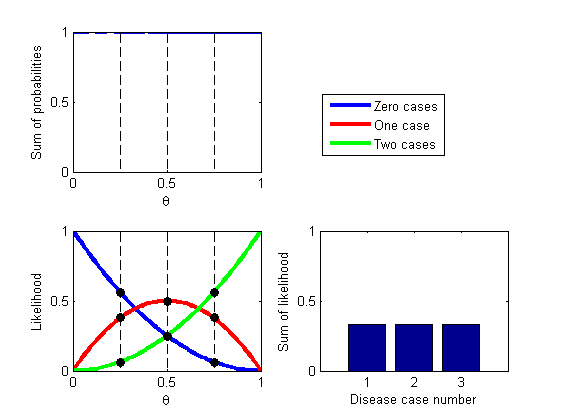
\includegraphics{likelihood_binomial.png}}
\caption{The likelihood function as theta varies for a sample of 2 individuals.}\label{fig:Likelihood_binomial}
\end{figure}

We will now extend the analysis to cover the case when we have groups of $N$ individuals. Firstly, consider the case when we have a group size of 3. If we assume that the individuals are identically distributed, then the 4 probabilities are of the form:

\begin{equation}\label{eq:Likelihood_binomialThreeProbsSimpler}
\begin{align}
P(Z = 0|\theta)& = \;P(X_1=0|\theta) P(X_2=0|\theta)  P(X_3=0|\theta)\\
P(Z = 1|\theta)& = 3P(X_1=1|\theta) P(X_2=0|\theta)  P(X_3=0|\theta)\\
P(Z = 2|\theta)& = 3P(X_1=1|\theta) P(X_2=1|\theta)  P(X_3=0|\theta)\\
P(Z = 3|\theta)& = \;P(X_1=1|\theta)P(X_2=1|\theta) P(X_3=1|\theta)
\end{align}
\end{equation}

Again, we notice a numeric pattern in terms of the first part of each expression $\{1,3,3,1\}$, which happens to correspond exactly to the coefficients on terms for the expansion of $(x+1)^3$. Hence, we can again rewrite the likelihood using the binomial expansion notation:

\begin{equation}\label{eq:Likelihood_binomialThreeFull}
P(Z=\beta|\theta) = {3 \choose \beta} \theta^\beta (1-\theta)^{3-\beta}
\end{equation}

We recognise a pattern in the likelihoods of (\ref{eq:Likelihood_binomialTwoFull}) and (\ref{eq:Likelihood_binomialThreeFull}) which allows us to deduce that, for a sample size of N, the likelihood is given by:

\begin{equation}\label{eq:Likelihood_binomialNFull}
P(Z=\beta|\theta) = {N \choose \beta} \theta^\beta (1-\theta)^{N-\beta}
\end{equation}

(\ref{eq:Likelihood_binomialNFull}) is known as the \textit{binomial} probability distribution.

If we had data, then we could test whether the assumptions made were appropriate by calculating the model-implied-probability of this outcome. For example, if we had a sample of 100 people of which 10 were disease-positive, and we assumed beforehand that the proportion of the population who have the disease is $\theta=1\%$, then we could calculate the probability that we would have achieved a number of cases as bad, or worse than this using (\ref{eq:Likelihood_binomialNFull}):

\begin{equation}
P(Z\geq 10|\theta=0.01) = \sum\limits_{Z=10}^{100}{100 \choose Z} 0.01^Z (1-0.01)^{100-Z} = 7.63 \times 10^{-8}
\end{equation}\label{eq:Likelihood_binomialTest}

We have summed over all the disease cases from 10 to 100 here, because we wanted the probability that we would have obtained a result as bad, or worse, than the one which we actually achieved. This is a particular way of carrying out classical hypothesis tests, which we will dispense with later on, but for now it seems a reasonable way of testing our model. 

The probability found in this case is extremely small. What does this tell us? Well, it basically says that there is something wrong with our model which we have chosen here. It could be that the actual disease incidence in the population is much higher than the 1\% which we have assumed beforehand. It could also be that our assumption \textit{independence} is violated in this case, for example if we sampled whole households rather than individuals. This could mean that in a particular household, the chance of having the disease, if another member of your family has the disease, is substantially higher than for the population as a whole. 

It is difficult to gauge what in particular is wrong with our model without knowing further details of data collection as well as how the estimate of 1\% incidence was estimated for the population. However, it does suggest that we need to do adjust one or more of our assumptions, and reformulate the model to take these into account. We should never simply accept that our model is \textit{correct}. A model is only as good as its capability to reproduce the data which we see in real life. In this case we find it is not a good representation, and we should readjust appropriately.

\subsection{The intelligence of a group of people}\label{sec:Likelihood_normal}
We are now tasked with formulating a model of intelligence test scores for a group of individuals for whom we have data. We are told that the test score is on a continuous scale from 0-200. We do not have any information on individual characteristics which might help us to predict scores, although we are going to, for this simplified example, assume that we do know the mean test score $\mu=70$, and its variance $\sigma^2=81$ in the population (although we will relax this assumption in section \ref{sec:Likelihood_MLE}). We might assume that there are a range of factors which overall result in an individual's performance on this test. For example, these might include their schooling, parental education, 'innate' ability, as well as how tired they were feeling on the day of the test. If we assume that there are a large range of such factors and the score which results is an average of all these, then we might assume that the Central Limit Theorem might be appropriate for determining the distribution of test scores. Don't worry if you are not aware of this theorem, we will cover it in due course, but basically it says, if there are a large number of factors whose average results in an intelligence score, then the normal distribution provides a reasonable approximation to the distribution of test scores. In which case, we assume that a normal distribution for our likelihood function for an individual's test score, $X$:

\begin{equation}
P(X=\alpha|\mu,\sigma^2) = \frac{1}{\sqrt{2\pi\sigma^2}}e^{-\frac{(\alpha-\mu)^2}{2\sigma^2}}
\end{equation}\label{eq:Likelihood_normal}

\begin{figure}
\centering
\scalebox{0.35} 
{\includegraphics{likelihood_normal.pdf}}
\caption{Left panel shows a normal with $\mu=70$ and $\sigma^2 = 81$, with the area corresponding to a result as extreme as 90 indicated. This translates into a standard normal cdf shown in the right panel, which can be used to calculate this area from the first figure. This translation to the standard normal is done by taking away $\mu$, and dividing through by $\sigma$. This is done since usually only standard normal cdf tables are available.}\label{fig:Likelihood_normal}
\end{figure}

If we obtain an individual within our sample who achieved a test score of 90, we ask what's the probability of achieving a result as extreme as this? Using our idealised model, we just integrate the probability density (this is the continuous analogue to the discrete summing that we did in (\ref{eq:Likelihood_binomialTest})):

\begin{equation}
\begin{align}
P(X\geq 90|\mu=70,\sigma^2=81) &= \int\limits_{90}^{\infty}\frac{1}{\sqrt{2\pi\times 10}}e^{-\frac{(\alpha-70)^2}{2\times 10}} \mathrm{d}\alpha\\
 & = 1-\Phi\left(\frac{90-70}{9}\right) \approx 0.0131
\end{align}\label{eq:Likelihood_normalSampleOne}
\end{equation}

In (\ref{eq:Likelihood_normalSampleOne}), $\Phi$ stands for the value of the \textit{standard} normal cumulative distribution function\footnote{A standard normal has mean 0, and a variance of 1. By taking away the mean of 70, and dividing through by the standard deviation, we transform from an arbitrary mean- and variance-normal, to a \textit{standard} one.} at the value of 90 (see figure \ref{fig:Likelihood_normal} for an explanation). Since we find that the probability of obtaining this data point under our current model is extremely small, we conclude that there is something wrong with our model, and go back to examine the various assumptions that were made in deriving it.

If we also assume that information regarding one individual's test score tells us nothing about another's\footnote{Apart from their joint reliance on $\mu$ and $\sigma^2$.}, then we might assume \textit{independence} for our data. We might also assume that all individuals come from the same population; resulting in a random sample. We calculate the joint probability density for a sample of N individuals by multiplying together the individual densities:


\begin{equation}
P(X_1=\alpha_1,X_2 =\alpha_2,...,X_N=\alpha_N|\mu,\sigma^2) = \prod\limits_{i=1}^{N}\frac{1}{\sqrt{2\pi\sigma^2}}e^{-\frac{(\alpha_i-\mu)^2}{2\sigma^2}}
\end{equation}\label{eq:Likelihood_normalN}


We could then use (\ref{eq:Likelihood_normalN}) to calculate the probability of obtaining a given sample of observations as extreme as the values obtained, again by integrating. However, here it would be slightly more complicated than that of (\ref{eq:Likelihood_normalSampleOne}) since we would have to integrate across all individuals' variables.

\section{The subjectivity of model choice}
It is hoped that the analysis in the preceding sections has given us a taste of how we can go about specifying a likelihood for a hitherto unknown circumstance. We start by writing down the behaviours that we want to emulate, then make simplifying assumptions, which we then use to look for an appropriate model in the literature. This model is then used to test the validity of the assumptions with the sample data. If the model struggles to explain the data, then we should go back and iteratively modify, then test our model, until it adequately explains the range of behaviours.

However, it should be re-emphasised that by its nature, a model is always a simplification of reality. As such, no one model is \textit{correct}. There are often many models that could be used to explain the data which we have to hand. We should always take care to test each of these against its ability to explain the aspect of the data with which we are interested, and only proceed with it if it is adequate in this regard. Real life is complicated, and thus with each of the assumptions that were used to justify a particular model, there will inevitably be a degree of \textit{subjectivity}. As such, no analysis - whether frequentist or Bayesian - can be thought to be purely \textit{objective}. Hence, the human analyst cannot, and should not, be replaced by automata for statistical analysis. A degree of subjective judgement is always necessary in statistics, as in all other walks of life.

\section{Maximum likelihood - a short introduction}\label{sec:Likelihood_MLE}
The analysis in section \ref{sec:chooseLikelihood} assumes that we know beforehand the fraction, $\theta$, of the populous that are predisposed to having the disease. In reality we rarely know such a thing. Often the main focus of building a statistical model is to try to estimate such parameters from our sample of data to which we have access. A popular frequentist method for achieving this goal is the estimation strategy known as \textit{Maximum Likelihood}. In this section we will examine how this estimation strategy yields estimates of parameters, as well as how these estimates can be used to make inferences about the population.

The principle of Maximum Likelihood estimation is simple. Firstly, we assume a model which we use to approximate the data generating process which resulted in our sample, based on the various assumptions about the real life process which we make. We then calculate what is known as the joint probability of obtaining the sample of observations, assuming that we do not know the parameters which specify completely those distributions. We then choose the parameters which \textit{maximise} the likelihood of obtaining that particular sample of observations. We will go through some simple examples to illustrate this process. 

\subsection{Estimating disease prevalence}\label{sec:Likelihood_diseaseMLE}
In section \ref{sec:Likelihood_diseaseGroup} we assumed that we knew beforehand the fraction of individuals who are disease-positive within the population. As mentioned previously, it is uncommon that such a thing be known before carrying out an analysis. If in a sample of 100 individuals, 10 test positively\footnote{Assuming for simplicity that there are no false-positives}, and we make the same assumptions as in section \ref{sec:Likelihood_diseaseGroup} - that of a random sample - then we can write down the overall likelihood function using (\ref{eq:Likelihood_binomialNFull}) as:

\begin{equation}\label{eq:Likelihood_binomialNew}
L(\theta|data) = {100 \choose 10} \theta^{10} (1-\theta)^{100-10}
\end{equation}

\begin{figure}
\centering
\scalebox{0.75} 
{\includegraphics{likelihood_logMonotonicity.png}}
\caption{A figure with four panes. The top-left is log-likelihood as a function of likelihood. The bottom-left is likelihood as a function of theta, and log-likelihood plotted on the same axis. Top-right is a weird function of likelihood as a function of likelihood. Below it a graph of likelihood as a function of theta, with a different maximum reached for the weird function.}\label{fig:Likelihood_logMonotonicity}
\end{figure}

Remember, that since we are varying $\theta$ and holding the data constant here, that (\ref{eq:Likelihood_binomialNew}) is a \textit{likelihood}, not a probability. We then need to simply choose $\theta$ so that we can maximise the likelihood. We could simply differentiate (\ref{eq:Likelihood_binomialNew}) as it stands, and set the derivative equal to 0; rearranging the resultant equation for $\theta$. However, to make life a little easier for us, we are first going to take the \textit{log} of this expression, then differentiate it, setting the derivative to 0; resulting in the same value of $\theta$. We are able to do this because of the simple properties of the log transformation (see figure \ref{fig:Likelihood_logMonotonicity}):

\begin{equation}\label{eq:Likelihood_logLikelihoodBinomial}
l(\theta|data) = Log L(\theta|data) = log{100 \choose 10}+ 10log(\theta)+ 90 log(1-\theta)
\end{equation}

Where to get the result (\ref{eq:Likelihood_logLikelihoodBinomial}), we have used the log rules:

\begin{equation}\label{eq:Likelihood_logRules}
\begin{align}
log(ab) &= log(a) + log(b)\\
log(a^b) &= blog(a)
\end{align}
\end{equation}

We can now simply differentiate the log-likelihood $l(\theta|data)$:

\begin{equation}\label{eq:Likelihood_binomialderiv}
\frac{\partial l}{\partial \theta} = \frac{10}{\hat{\theta}}-\frac{90}{1-\hat{\theta}} = 0
\end{equation}

If we set the derivative to 0 we then obtain the maximum likelihood \textit{estimate}, $\hat{\theta} = \frac{1}{10}$ (see figure \ref{fig:Likelihood_MLE}).

\begin{figure}
\centering
\scalebox{0.75} 
{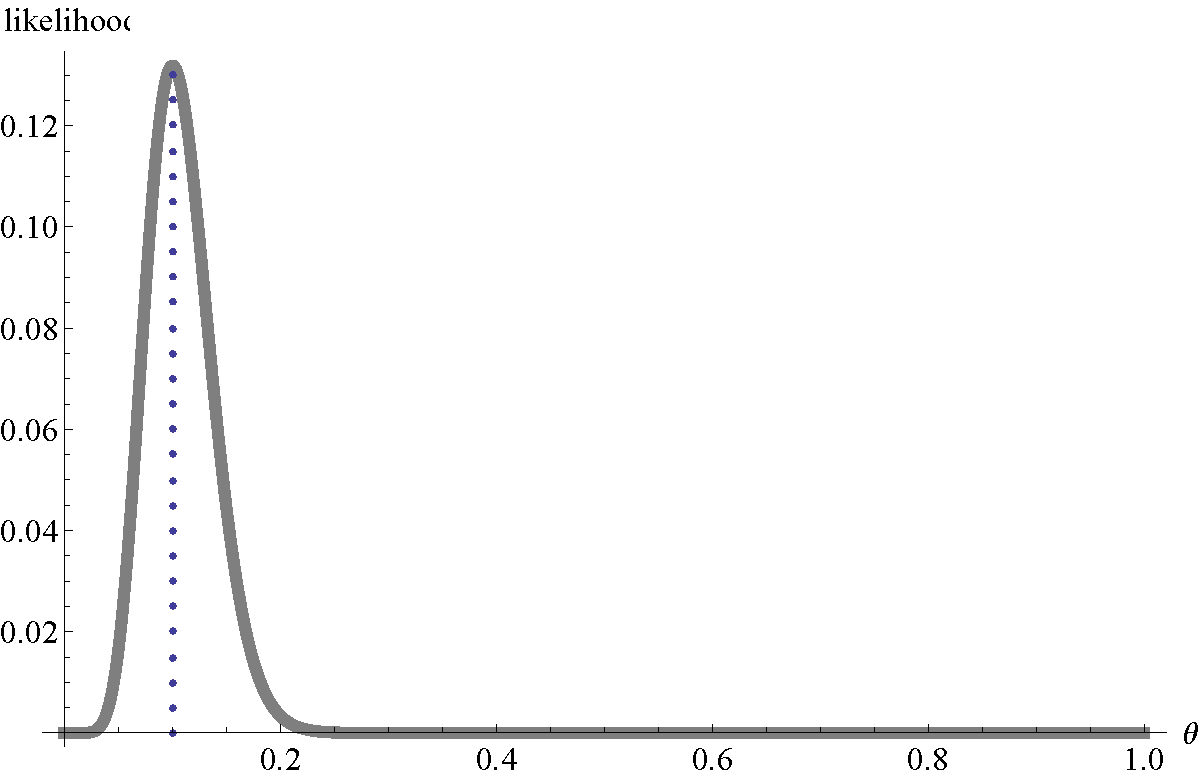
\includegraphics{Likelihood_ML.pdf}}
\caption{Log-likelihood of disease prevalence from section \ref{sec:Likelihood_diseaseMLE} as a function of theta, maximised at 1/10.}\label{fig:Likelihood_MLE}
\end{figure}


This estimator makes sense intuitively. The value of the parameter which results in the highest likelihood of obtaining the data occurs when the population prevalence exactly matches that obtained in our sample. In general if we found a number $\beta$ of individuals out of a sample of size $N$, who were disease-positive, then we would again find that the preceding analysis results in an estimator\footnote{An estimator is a mathematical function which outputs an estimate of a parameter in our model.} of the disease prevalence exactly equal to that in our sample:

\begin{equation}\label{eq:Likelihood_binomialestimator}
\hat{\theta} = \frac{\beta}{N}
\end{equation}

\subsection{Estimating the mean and variance in intelligence scores}
We are given a sample of individuals with test scores $\{75,71\}$, and we model the test scores using a normal likelihood as described in section \ref{sec:Likelihood_normal}:

\begin{equation}\label{eq:Likelihood_normalTwo}
L(\mu,\sigma^2|X_1=75,X_2 =71) = \frac{1}{\sqrt{2\pi\sigma^2}}e^{-\frac{(75-\mu)^2}{2\sigma^2}}\times \frac{1}{\sqrt{2\pi\sigma^2}}e^{-\frac{(71-\mu)^2}{2\sigma^2}}
\end{equation}

We can then proceed as we did in section \ref{sec:Likelihood_diseaseMLE} by taking the log of this expression before we differentiate it:

\begin{equation}\label{eq:Likelihood_diseaseLogLikelihood}
l(\mu,\sigma^2|X_1=75,X_2 =71) = 2log\left(\frac{1}{\sqrt{2\pi\sigma^2}}\right)-{\frac{(75-\mu)^2}{2\sigma^2}}-{\frac{(71-\mu)^2}{2\sigma^2}}
\end{equation}

Where we have again used the log rules in (\ref{eq:Likelihood_logRules}) to achieve (\ref{eq:Likelihood_diseaseLogLikelihood}). We can now proceed to differentiate (\ref{eq:Likelihood_diseaseLogLikelihood}) with respect to both variables, holding the other constant, setting each to 0:

\begin{equation}\label{eq:Likelihood_diseaseDerivativeOne}
\begin{align}
\frac{\partial l}{\partial \mu} &= {\frac{(75-\hat{\mu})}{\hat{\sigma^2}}}+{\frac{(71-\hat{\mu})}{\hat{\sigma^2}}} = 0\\
\frac{\partial l}{\partial \sigma^2} &= -\frac{1}{\hat{\sigma^2}} + \frac{(75-\hat{\mu})^2+(71-\hat{\mu})^2}{2\hat{\sigma^4}} = 0
\end{align}
\end{equation}

The first of these expressions yields $\hat{\mu} = \frac{71+75}{2} = 73$, which when put into the second gives: 

\begin{equation}
\hat{\sigma^2} = \frac{1}{2}\left[(75-73)^2 + (71-73)^2)\right] = 4
\end{equation}

Notice that the maximum likelihood estimators for the population mean and variance are for this case the \textit{sample mean} and \textit{sample variance}\footnote{Albeit a biased estimator of the population variance. The unbiased estimator would divide by 1, rather than 2.}. In fact, this holds for the case of N individuals' data, then the maximum likelihood estimators for this case would be:

\begin{equation}
\hat{\mu} = \frac{1}{N}\sum\limits_{i=1}^{N} X_i = \bar{X}
\end{equation}
\begin{equation}
\hat{\sigma^2} = \frac{1}{N}\sum\limits_{i=1}^{N}(X_i-\bar{X})^2 = s^2
\end{equation}

\section{Frequentist inference in Maximum Likelihood}
We have now detailed how to derive point estimates of parameters using the method of maximum likelihood. However, at the moment we are unable to make any conclusions about the population. This is because we do not have any idea as to whether we obtained a particular estimate of a parameter due to picking a weird sample, or because it \textit{actually} has a value in the population which is at this value. Frequentists get round this by examining a graph of log-likelihood near the maximum likelihood point estimate (see figure \ref{fig:Likelihood_likelihoodCurvature}). If the log-likelihood is strongly peaked near the maximum likelihood estimate, then this suggests that only a small range of parameters would yield a similar valued likelihood. By contrast, if the log-likelihood is gently peaked near the ML estimate, then it is feasible that a large range of parameters would yield estimates close to this value. In the latter case, it seems logical that we should be less confident in the particular value of the parameter which is given by maximum likelihood. We can measure the 'peakedness' in the log-likelihood by looking at the magnitude of the second derivative\footnote{The first derivative gives the gradient, the second derivative gives the rate of change of the gradient - a measure of curvature.} of the function at the ML point estimate value. The more curved the log-likelihood, the more confident we can be of our estimated parameter value, and any conclusions drawn from this. Note however, that the frequentist inference is not based on proper probability distributions (since we infer based on a likelihood). This contrasts with the Bayesian method which, by its nature, allows for a more adequate description of parameters, using probability distributions.

\begin{figure}
\centering
\scalebox{0.65} 
{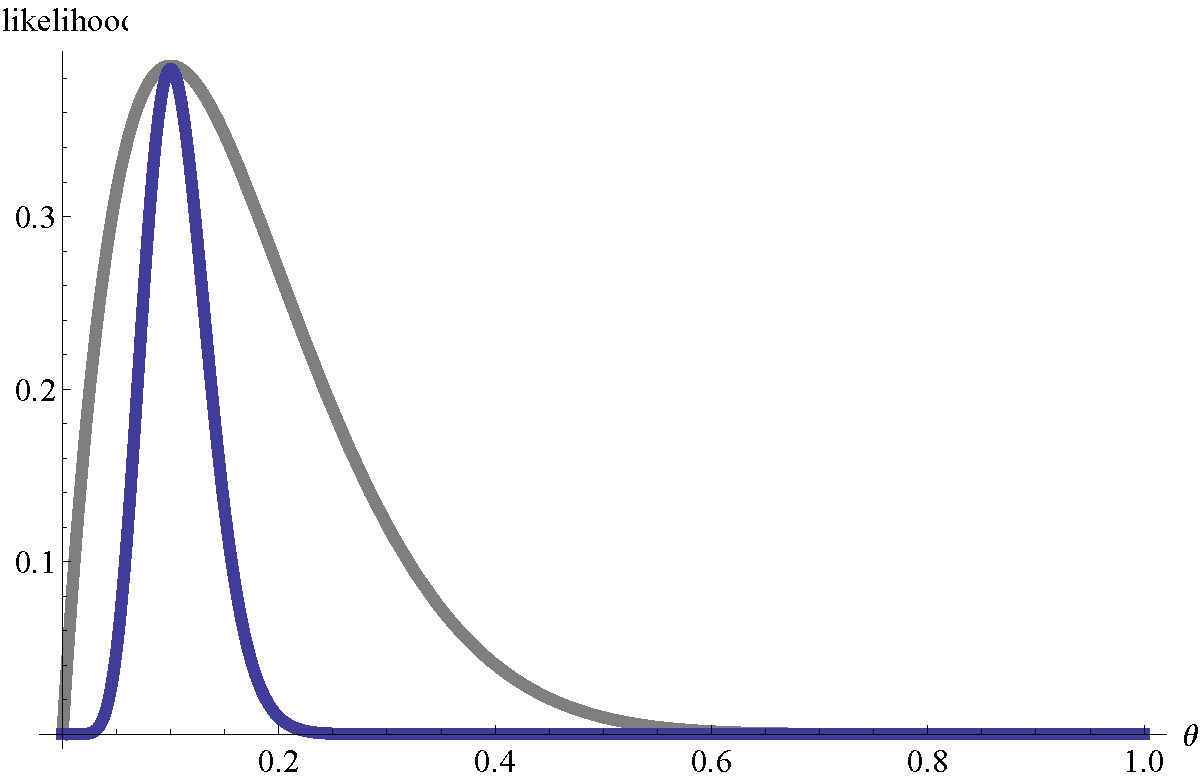
\includegraphics{Likelihood_likelihoodCurvature.pdf}}
\caption{Two likelihoods which result in the same maximum likelihood estimates of parameters, at 0.1. The gray likelihood is less strongly-peaked, meaning we can be less confident about the estimates.}\label{fig:Likelihood_likelihoodCurvature}
\end{figure}


\section{Chapter summary}
We should now understand what is meant by a likelihood, and how to build probabilistic models of real life processes. However, the difficulty of modelling a process is governed by its degree of complexity and sensitivity to violations of assumptions. Further we should also understand how the frequentist method of Maximum Likelihood can be used to yield point estimates of parameters. We are however, currently restricted in our ability to make inferences based on full probability distributions over parameters. Bayes' rule tells us how we can convert a likelihood - itself not a proper probability distribution - to a posterior (\textit{correct}) probability distribution for parameters. In order to use to do this though, we need to understand what is meant by a \textit{prior} distribution and how we can specify this distribution to suit the particular situation. This is what is covered in the next chapter.

\chapter{Priors}\label{chap:Prior}
\section{Chapter Mission statement}
At the end of this chapter a reader will know what is meant by a prior, and the different philosophies that are used to understand and construct them. 

Insert a graphic with the likelihood part of Bayes' formula circled, as in the equation shown below for the part highlighted in blue.

\begin{equation}
P(\theta|data) = \frac{P(data|\theta)\times {\color{blue}P(\theta)}}{P(data)}
\end{equation}\label{eq:Prior_BayesHighlighted}

\section{Chapter goals}
Bayes' rule tells us how to convert a likelihood - itself not a proper probability distribution - into a posterior probability distribution for parameters, which can then be used for inference. We are required in the numerator to multiply the likelihood by a pre-experimental weighting of each set of parameter values described by a probability distribution, which is known as a \textit{prior}. Priors are without doubt the most controversial aspect of Bayesian statistics, with its opponents criticising its inherent \textit{subjectivity}. It is hoped that by the end of the chapter we will have convinced the reader that, not only is subjectivity inherent in \textit{all} statistical models - both frequentist and Bayesian - but the explicit subjectivity of priors is more transparent, and hence open to interrogation, than the implicit subjectivity abound elsewhere.

This chapter will also explain the differing interpretations which are ascribed to priors. The reader will come to understand the types of method that can be used to construct prior distributions, and how they can be chosen to be minimally subjective, or otherwise to contain informative pre-experimental insights from data or opinion. Finally, the reader will understand that if significant data are available then the conclusions drawn should be insensitive to the initial choice of prior.

Inevitably, this chapter will be slightly more philosophical and abstract than other parts of this book, but it is hoped that the examples given will be sufficient to ensure its practical use.

\section{What are priors, and what do they represent?}
Chapter \ref{chap:Likelihoods} introduced us to the concept of formulating a likelihood, and how this can be used to derive frequentist estimates of parameters, using the method of maximum likelihood. This pre-supposes that the parameters in question are immutable, fixed quantities that actually exist, and can be estimated by methods that can be repeated, or imagined to be repeated many times \cite{gill2007bayesian}. As Gill (2007) indicates, this is unrealistic for the vast majority of social science research.

\begin{quotation}
It is simply not possible to rerun elections, repeat surveys under exactly the same conditions, replay the stock market with exactly matching market forces, or re-expose clinical subjects to identical stimuli.
\end{quotation}

Furthermore, parameters only exist because we have \textit{invented} a model, hence we should innately be suspicious of any analysis which assumes an existence of a single certain value for any aspect of these abstractions.

For Bayesians, it is the data that are treated as fixed, and the parameters that vary. We know that the likelhood - however useful - is not a proper probability distribution. Bayes' rule tells us how to combine a likelihood with something called a \textit{prior} to obtain a proper posterior distribution for the parameter in question, which can then be used for inference. But what does it actually mean for a parameter to have a prior distribution?

Gelman et al. (2013) suggests that there are two different interpretations of priors: the \textit{state of knowledge} interpretation, where we specify our knowledge and uncertainty in a parameter as if regarding it as a draw from a probability distribution; alternatively in the more objective \textit{population} interpretation where the current value of a parameter is the result of a draw from a true population distribution \cite{gelman2013bayesian}. In both viewpoints the model parameters are not viewed as static, unwavering constants as they are taken to be in frequentist theory.

\begin{figure}
\centering
\scalebox{0.3} 
{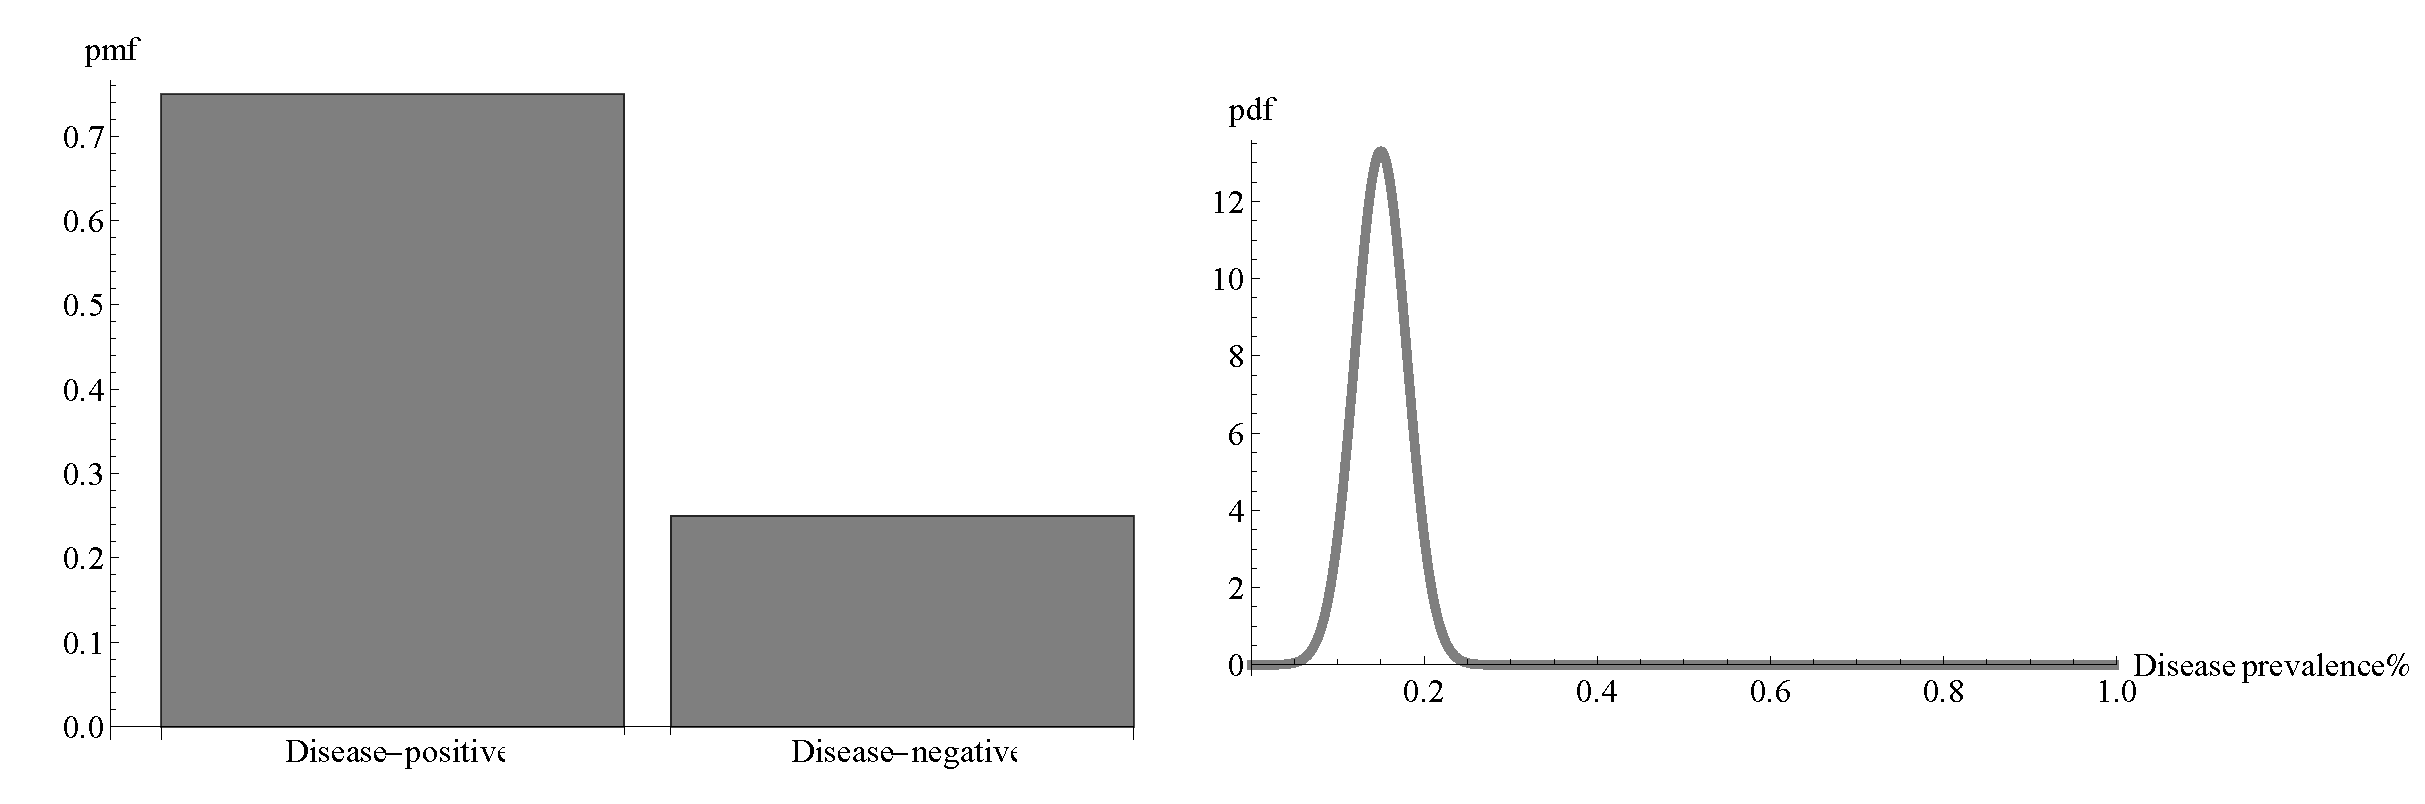
\includegraphics{Prior_introduction.pdf}}
\caption{Left - a prior for a doctor's pre-testing diagnostic probability of an individual having a disease. Right - a prior which represents pre-sample uncertainty in disease prevalence.}\label{fig:Prior_introduction}
\end{figure}

If we adopt the \textit{subjective} viewpoint above, then we can think of the prior as representing our pre-experimental/data certainty in the parameter in question. For example, imagine that a Doctor is asked to evaluate the probability before the results of a blood test become available, that a given individual has a particular disease. Using their knowledge of the patient's history and their expertise on the particular condition, they assign a prior disease probability of 75\% (see figure \ref{fig:Prior_introduction}). 

Alternatively, imagine we are tasked with estimating the proportion of the UK population that has a particular disorder. We may have some idea of its prevalence, as well as the variance in the mean prevalence of a disease across a range of previous samples of individuals which have been tested. In this case, the prior is continuous and represents our uncertainty in our estimate of the prevalence (see figure \ref{fig:Prior_introduction}). In all cases a prior is a proper probability distribution, and hence can be used to elicit our prior expectations as to the value of a parameter. For example, we could use the prior probability distribution for the proportion of individuals having a particular disorder in figure \ref{fig:Prior_introduction} to estimate a pre-experimental mean of approximately 15\% prevalence.

Adopting the \textit{population} perspective described by Gelman, we imagine the value of a parameter of current interest to be drawn from a population distribution. If we imagine the process of flipping a coin, we could if we knew the angle at which it is tossed, as well as the height from which it is thrown above the surface\footnote{Also assuming that we knew the physical properties of the coin and surface.} predict deterministically the side on which the coin would fall face up. We could then hypothetically enumerate the (infinitely) many angles and heights of the coin, and for each set determine whether the coin would fall face up or down. Each time we throw the coin we are implicitly choosing an angle and height from the set of all possible combinations, which determines whether a heads or tails falls face up. Some ranges of the angle and the height will be more frequently chosen than others, albeit relatively agnostic with regards to final state of the coin.  Hence we could think of this choice as the realisation from a distribution of all possible sets. Thus we could think about the choice of angle and height as being a realisation from this \textit{population} distribution, and hence determines the fate of the coin toss.

\section{Why don't we just normalise likelihood by choosing a unity prior?}\label{sec:Prior_unityPrior}
Why can't we simply let the prior be unity for all values of $\theta$, in other words set $P(\theta) = 1$ in the numerator of Bayes' rule; resulting in a posterior that takes the form of a normalised likelihood:

\begin{equation}
P(\theta|data) = \frac{P(data|\theta)} {P(data)}
\end{equation}\label{eq:Prior_BayesNormalisedLikelihood}


This would surely negate the need for specification of a prior, and thwart all attempts to denounce Bayesian statistics as \textit{subjective}. So why don't we do just that? 

There is a pedantic, mathematical argument against this, which is that $P(\theta)$ must be a proper probability distribution to ensure the same properness of the posterior. If we choose $P(\theta) = 1$ (or in fact any positive constant), then the integral $\int\limits_{-\infty}^{+\infty}P(\theta)\mathrm{d}\theta\rightarrow\infty$, and we can no longer think of the distribution, $P(\theta)$ as representing a probability. It may still be possible that even if the prior is improper, that the resultant posterior also satisfies the required properties of a proper probability distribution, but care must be taken when using these distributions for inference, as technically they are \textit{not} probability distributions, due to the abuse of Bayes' rule. In this case the posteriors can only be viewed at best as approximations to the result we would have obtained under some limiting prior distribution.

Another, perhaps more persuasive argument, is that by assuming all parameter sets have an equal likelihood of being chosen beforehand, then this can result in nonsensical resultant conclusions being drawn. Consider the following example: 

We are given some data on a coin which has been flipped twice, with the result $\{H,H\}$. We are given the choice of deciding whether the  coin is fair, with an equal chance of both heads and tails occurring, or biased with a very strong weighting towards heads. We denote fairness by a parameter $theta=1$, if the coin is fair, and $theta=0$ otherwise.

\begin{figure}
\centering
\scalebox{0.75} 
{\includegraphics{Prior_justification.png}}
\caption{A figure showing in the left hand panel the Venn diagrams when we assume that a) the coin is fair with a quarter of the area shaded, and the other half not. b) Biased, and the majority of the figure is shaded - corresponding to a high overlap between data and parameter. The right hand panel then shows the joint probability of the data and the parameters $\theta$, and we see that even though the ratio of the area is better for b), it is much less likely \textit{a priori} that the coin is biased. The bottom panel shows the ML implied posterior distribution, with the bar for unfairness much higher than for fairness. The right shows a much more logical conclusion which takes into account their prior probabilities.}\label{fig:Prior_justification}
\end{figure}

Figure \ref{fig:Prior_justification} illustrates how assuming an improper uniform prior in this case results in a very strong posterior weighting towards the coin being biased. This is because from a likelihood perspective - $P(data|\theta)$ - if we assume that the coin is biased, then the probability of obtaining two heads is high. Whereas if we assume that the coin is fair, then the probability of obtaining this data is only $\frac{1}{4}$. Thus, by ignoring common sense - that it is likely the majority of coins are relatively unbiased - we end up with a result that is nonsensical. 

Of course, in this example we would hope that by collecting more data, in this case, throws of the coin, we could be confident in the conclusions drawn from the likelihood. However, Bayesian analysis allows us to achieve such a goal with a smaller sample size, should we be relatively confident about our pre-data knowledge.

\section{The explicit subjectivity of priors}
Opponents of Bayesian approaches to inference criticise the subjectivity inherent with choice of prior. However, all analysis involves a degree of subjectivity, particularly in regard to choice of statistical model. This choice is often formulated implicitly as being \textit{objectively} correct, with little justification or discourse given to the underlying assumptions necessary to arrive there. The statement of a prior, necessary for any full description of a Bayesian analysis, is at least \textit{explicit}; leaving this aspect of the modelling subject to the same interrogation and academic examination to which any analysis should be subjected. A word that is often used by protagonists of Bayesian methods, is that it is \textit{honest} due to the \textit{explicit} statement of assumptions. The statement of pre-experimental biases actually forces the analyst to self-examine, and perhaps also leads to a decline in the temptation to manipulate the analysis to one's own ends.



\section{Combining a prior and likelihood to form a posterior} 
This chapter thus far has given more attention to the philosophical and theoretical underpinnings of Bayesian analysis. Now we change tack to illustrate to the reader the mechanics behind Bayes' formula; specifically how the prior is combined with the likelihood to yield a posterior probability distribution. The following examples introduce an illustrative method, known as \textit{Bayes' box} described in detail in \cite{stewart2014teaching} and \cite{bolstad2007introduction}, which illustrates the functioning of Bayes' rule, in which the parameter, prior, likelihood, and posterior are all displayed in a logical manner.

\subsection{An urn of balls\footnote{Taken from Bolstad's great introduction to Bayesian statistics \cite{bolstad2007introduction}.}}\label{sec:Prior_urn}
Imagine an urn of 5 balls, each of which is red or white, and suppose we are tasked with inferring the total number of red balls which are present in the urn, on the basis of a single ball which we pick out, and find to be red. Before we pull the ball out from the urn, we have no prejudice for a particular number of red balls, and so suppose that all possibilities - 0 to 5 - are equally likely, and hence have the probability of $\frac{1}{6}$ in our discrete prior. Our model for the likelihood is that a number $Y$ of the balls are red, and that the result of an individual picking of a ball from the urn tells us nothing about future picks, apart from their joint dependence on $Y$. In this oversimplified example, this assumption of independence seems reasonable, particularly if the balls are picked out in a randomised manner and have no distinguishing features. Further suppose that the random variable $X\in\{0,1\}$ indicates whether the ball is white or red respectively.  The analogy with the disease status of an individual described in section \ref{sec:Likelihood_individualDisease} is evident, and hence we choose a likelihood of picking a red ball of the form:

\begin{equation}\label{eq:Prior_bernoulli}
P(X = 1|Y=\alpha) = \frac{\alpha}{5}
\end{equation}

In (\ref{eq:Prior_bernoulli}), $\alpha\in\{0,1,2,3,4,5\}$ represents the number of red balls in the urn.

We can then illustrate the functioning of Bayes' rule in the \textit{Bayes' box} shown in table \ref{tab:Prior_bayesBoxDiscreteUrns}. We start by listing all the possible numbers of red balls that can exist in the Urn in the leftmost column. We then introduce our prior probabilities that we associate with each of the six potential numbers of red balls that can be in the urn. In the third column we then calculate the likelihoods for each of the outcomes using the simple rule given in (\ref{eq:Prior_bernoulli}). We then multiply the prior by the likelihood in the fourth column, which on summation gives us $P(data)=\frac{1}{2}$, which we use to create a proper probability distribution for the posterior in the last column. For a mathematical description of this process see section \ref{app:Prior_bayesUrn}.

The Bayes' box illustrates the straightforward and mechanical working of Bayes' rule for the case of discrete data. We also note that when we sum the likelihood over all possible numbers of red balls in the urn - in this case the parameter which we are trying to infer - we find that this to be equal to 3; illustrating again that a likelihood is not a valid probability distribution. We also see that at a particular parameter value, if either the prior or the likelihood are found to be zero as is the case of 0 red balls being in the urn (impossible since we have at least one), then this ensures that the posterior distribution is zero at this point. This makes it important that we use a prior that gives a positive weight to \textit{all} possible ranges of parameter values. The results are also displayed graphically in figure \ref{fig:Prior_urnStacked}.

\begin{table}[htbp]
  \centering
  \caption{A Bayes' box showing how to calculate the posterior for the case of drawing balls from an urn containing 5 red and white balls, one of which has been drawn and shown to be red. Here we assume that pre-experiment all possible numbers of red balls are equally likely, by adopting a uniform prior.}\label{tab:Prior_bayesBoxDiscreteUrns}
    \begin{tabular}{ccccc}
    \toprule
    \textbf{Number of red balls} & \textbf{Prior} & \textbf{Likelihood} & \textbf{Prior x likelihood} & \textbf{Posterior$=\frac{Prior\times Likelihood}{P(data)}$} \\
    \midrule
    0     &  1/6  & 0     & 0       & 0       \\
    1     &  1/6  &  1/5  &   1/30 &   1/15 \\
    2     &  1/6  &  2/5  &   1/15 &   2/15 \\
    3     &  1/6  &  3/5  &   1/10 &   3/15  \\
    4     &  1/6  &  4/5  &   2/15 &   4/15 \\
    5     &  1/6  & 1     &   1/6  &   5/15  \\
    \bottomrule
    Total & \textbf{1    } & \textbf{3    } & \textbf{$P(data)=1/2$ } & \textbf{1      } \\
    \bottomrule
    \end{tabular}%
  \label{tab:addlabel}%
\end{table}%

\begin{figure}
\centering
\scalebox{0.75} 
{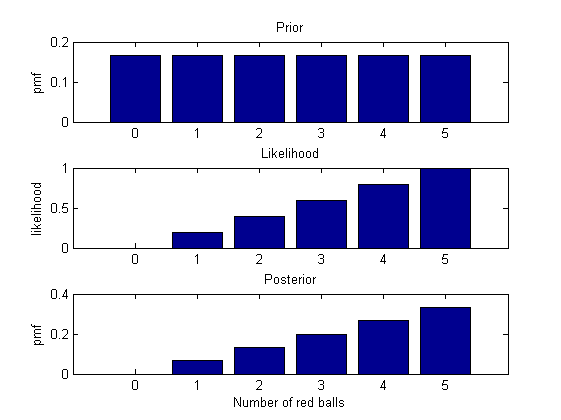
\includegraphics{Prior_urnStacked.png}}
\caption{The prior, likelihood and posterior for the urn of balls example described in \ref{sec:Prior_urn}. The prior in the upper panel gives uniform weighting to all possible numbers of red balls. This is then multiplied by the likelihood (in the middle panel) at each number of balls, and normalised to make the posterior density shown in the bottom panel.}\label{fig:Prior_urnStacked}
\end{figure}

Now suppose that we had reason to believe that the urn-maker had a prejudice towards more equal numbers of both balls, and as a result we alter our prior to have a greater weight towards these numbers of red balls (see table \ref{tab:Prior_bayesBoxUrnUpdated} and figure \ref{fig:Prior_bayesUrnUpdated}).


\begin{table}[htbp]
  \centering
  \caption{A Bayes' box showing how to calculate the posterior for the case of drawing balls from an urn containing 5 red and white balls, one of which has been drawn and shown to be red. Here a higher weighting is given to more equal numbers of red and white balls in the prior.}\label{tab:Prior_bayesBoxUrnUpdated}%
    \begin{tabular}{ccccc}
    \toprule
    \textbf{Number of red balls} & \textbf{Prior} & \textbf{Likelihood} & \textbf{Prior x likelihood} & \textbf{Posterior$=\frac{Prior\times Likelihood}{P(data)}$} \\
    \midrule
    0     &   1/12 & 0     & 0       & 0       \\
    1     &   1/6  &  1/5  &   1/30 &   1/15 \\
    2     &   1/4  &  2/5  &   1/10 &   1/5  \\
    3     &   1/4  &  3/5  &   3/20 &   3/10 \\
    4     &   1/6  &  4/5  &   2/15 &   4/15 \\
    5     &   1/12 & 1     &   1/12 &   1/6  \\
    \bottomrule
    Total & \textbf{1      } & \textbf{3    } & \textbf{  1/2 } & \textbf{1      } \\
    \bottomrule
    \end{tabular}%
  
\end{table}%

\begin{figure}
\centering
\scalebox{0.75} 
{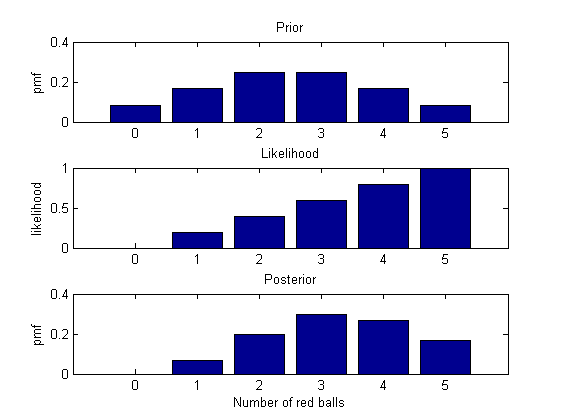
\includegraphics{Prior_bayesUrnUpdated.png}}\caption{The prior, likelihood and posterior for the urn of balls example described in \ref{sec:Prior_urn}. The prior in the upper panel gives more weighting to more equal numbers of red and white balls. This is then multiplied by the likelihood (in the middle panel) at each number of balls, and normalised to make the posterior density shown in the bottom panel.}\label{fig:Prior_bayesUrnUpdated}
\end{figure}


\subsection{Disease proportions revisited}\label{sec:Prior_diseaseProp}
Suppose that we substitute our urn from section \ref{sec:Prior_urn} for a sample of 100 individuals taken from the UK population. Suppose also that we continue to assert the independence of individuals within our sample, and make explicit the assumption that individuals are from the same population, and are hence identically-distributed. We are now interested in making conclusions about the overall proportion of individuals within the population who have the disease, $\theta$. Since the parameter of interest is now continuous, we cannot use Bayes' box as there would be infinitely many rows (corresponding to the continuum of possible $\theta$) over which to sum. Let's suppose that within our sample of 100 we find 3 of them who are disease-positive\footnote{We also suppose that there are no false-positives here.}. We could then use the assumptions of independence and identical-distribution to write down a likelihood of the form introduced in section \ref{sec:Likelihood_diseaseGroup}:

\begin{equation}\label{eq:Prior_binomial}
P(Z=3|\theta) = {100 \choose 3} \theta^\beta (1-\theta)^{100-3}
\end{equation}

The reason for the ${100 \choose 3}=161,700$ term at the beginning of (\ref{eq:Prior_binomial}) is that we have to count the number of different permutations of getting 3 individuals who are disease-positive within a sample size of 100. 

We suppose that at the beginning of the experiment all values of $\theta$ are equally likely. However, we would expect researchers to have a pre-experimental idea as to the most probable frequencies of the disease within the population, meaning that a flat prior which is given is likely understating a prejudice towards a certain range of $\theta$ values. Whilst, this is the case, it is often assumed in research papers - for the sake of objectivity - that priors are flat, in order to try to minimise the effect which assumptions here make on the outcome of an analysis.

\begin{figure}
\centering
\scalebox{0.75} 
{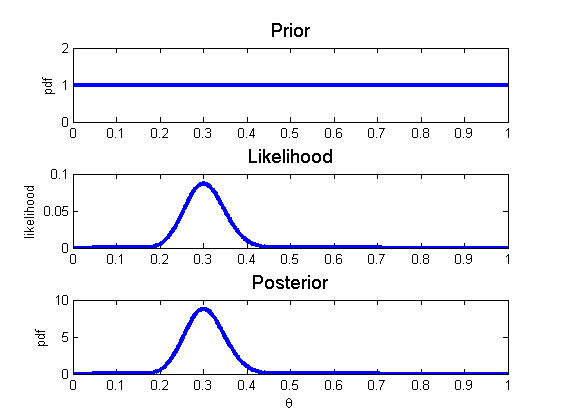
\includegraphics{Prior_disease.png}}
\caption{The prior, likelihood and posterior for the disease proportion example described in section \ref{sec:Prior_diseaseProp}. Each point in $\theta$ along the continuous prior curve (top panel) is multiplied by the corresponding value of likelihood (middle panel), to form the numerator of Bayes' rule. The numerator is then normalised to make the posterior probability density shown in the bottom panel.}\label{fig:Prior_disease}
\end{figure}

\section{Constructing priors}
There are a number of different methodologies and philosophies when it comes to the construction of a prior density. In this section we consider briefly how priors can be engineered so as to be relatively uninformative - better-termed vague - or alternatively can be used to assemble pre-experimental knowledge in a logical manner.

\subsection{Vague priors}\label{sec:Prior_vague}
When there is a premium placed on the objectivity of analysis, as is often the case in regulatory work - drug trials, public policy and the like - then use of a relatively 'uninformative' prior is often desired. If we were uncertain as to the proportion of individuals within a population who have a particular disease, then a uniform prior (see figure \ref{fig:Prior_jeffreysIntro}) is often employed to this end. 

The use of a prior that has a constant value, $P(\theta)=constant$, is attractive because in this case:

\begin{equation}
\begin{align}
P(\theta|data) &= \frac{P(\theta)\times P(data|\theta)}{P(data)}\\
& \propto P(\theta)\times P(data|\theta)\\
& \propto P(data|\theta)
\end{align}
\end{equation}\label{eq:Prior_BayesFlatPrior}

In (\ref{eq:Prior_BayesFlatPrior}) we thus see that the shape of the posterior distribution is solely determined by the likelihood function. This is seen as a merit of uniform priors since they 'let the data speak for itself' through the likelihood. This is used as the justification for using a flat prior in many analyses.

The flatness of the uniform prior distribution is often termed 'uninformative', but this is misleading. If we assume the same model as described in section \ref{sec:Prior_diseaseProp}, then the probability that one individual has the disease is $\theta$, and the probability that two randomly sampled individuals both have the disease is $\theta^2$. If we assume a flat prior for $\theta$, then this implies a decreasing prior shown in figure \ref{fig:Prior_jeffreysIntro} for $\theta^2$. Furthermore, when we consider the probability that within a sample of ten individuals, all of whom are diseased, we see that a flat prior for $\theta$ implies an even more accentuated prior for this event; meaning that we beforehand give little weight to this event. For the mathematical details of these graphs see section \ref{app:Prior_diseaseJeffreys}.

\begin{figure}
\centering
\scalebox{0.75} 
{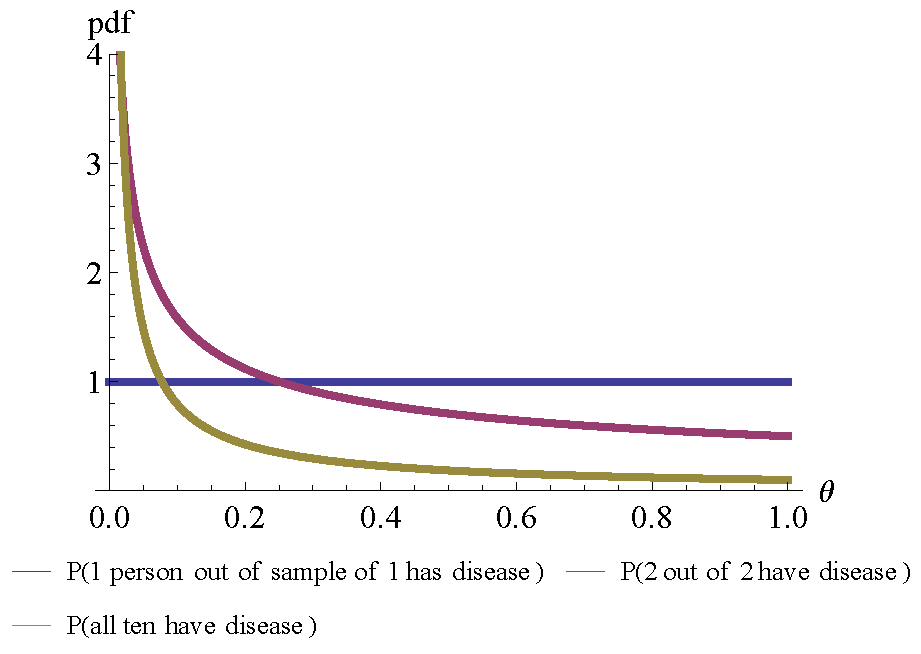
\includegraphics{Prior_jeffreysIntro.pdf}}\caption{The probability density for obtaining all diseased individuals within sample sizes of 1, 2 and 10 respectively. Starting out with a flat prior for the probability that one individual has a disease has resulted in non-flat priors for the other 2 probabilities.}\label{fig:Prior_jeffreysIntro}
\end{figure}

We can hence see that even though a uniform prior for an event looks, on first glances, to convey no information, we are actually making quite informative statements about other events. This aspect of choosing flat priors is swept under the carpet for most analyses, partly because often we care most about the particular parameter to which we create a prior. All priors contain some information, so we prefer the use of the terms "vague" or "diffuse" to represent situations where a premium is placed on drawing conclusions from only the data at hand.

There are methods for constructing priors that seek to limit the information contained within priors, so as to not colour the analysis with pre-experimental prejudices. However, we will leave a discussion of these methods until chapter \ref{chap:ObjectiveBayes} on \textit{Objective Bayes}.

Whilst uniform priors are relatively straightforward to specify when we aim to infer about a parameter which is bounded - such as in the previous example where $\theta\in\{0,1\}$, or in the case of discrete parameters - we run into issues for parameters which have no predefined range. An example of this would be if we were aiming to determine the mean, $\mu$, time of onset of lung cancer for individuals who develop the disease, after they begin to smoke. If we remove all background cases (assumed not to be caused by smoking), then $\mu$ has a lower bound of 0. However, there is no obvious point at which to draw an upper bound. A naive solution to this would be to use a prior for $\mu\sim Unif(0,\infty)$. This solution, although at first appears to be reasonable, is not viable for two reasons; one statistical, another which is practical. The statistical reason is that $\mu\sim Unif(0,\infty)$ is not a valid probability density, because any non-zero constant value for the pdf will mean that the area under the curve is $\infty$ because the $\mu$ axis stretches out forever. The common sense argument is that we would never ascribe the same likelihood to an individual having onset of lung cancer after 10 years as for it occurring after 250 years! The finiteness of human lifespan dictates that we select a more appropriate prior. If we were to ignore these two concerns although it is possible that the posterior could behave as a valid probability distribution\footnote{Although not assured.}, it would not actually be one (see section \ref{sec:Prior_unityPrior} for an explanation). A better choice of prior to use in this example would be one which ascribes zero probability to negative values of $\mu$, and ever decreasing values of the pdf for high values of $\mu$ such as the one shown in figure \ref{fig:Prior_lungcancerFlatandGammaPriors}. Alternatively, we could choose a uniform prior on a reasonable range of $\mu$, and allow the pdf to be zero elsewhere (see figure \ref{fig:Prior_lungcancerFlatandGammaPriors}).


\begin{figure}
\centering
\scalebox{0.75} 
{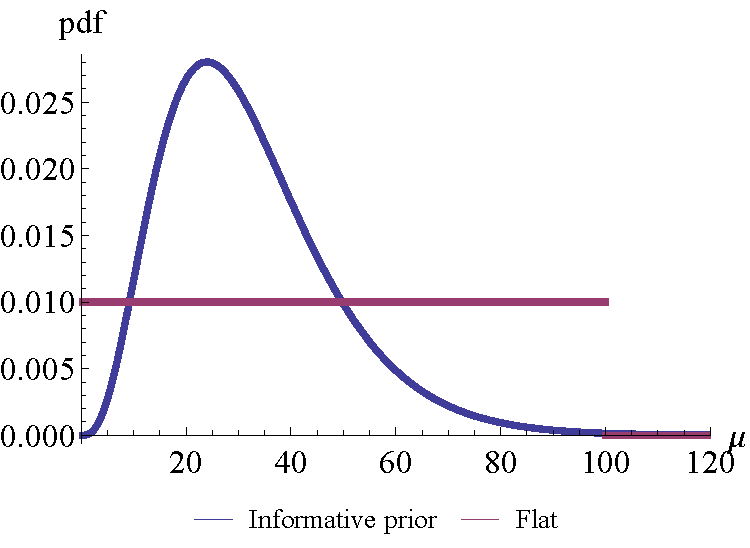
\includegraphics{Prior_lungcancerFlatandGammaPriors.pdf}}\caption{Two viable prior distributions for the average time taken before the onset of lung cancer after patients begin smoking.}\label{fig:Prior_lungcancerFlatandGammaPriors}
\end{figure}

\subsection{Informative priors}
We have seen in section \ref{sec:Prior_vague} that priors are frequently chosen to give a strong voice to the recent data; minimising the impact of existing prejudices. There are however occasions when the choice of prior acknowledges that the analysis is based on more than the latest data. This choice of prior can be used to incorporate previous data, conclusions from older studies, or to include expert opinion. 

In cases where data is available from previous studies, the construction of a prior can proceed methodically via a method that is known as \textit{moment-matching}. Suppose that we have the data shown in figure \ref{fig:Prior_SATScoresHistogram} for SAT scores of past participants of a particular class. We might think that to a reasonable approximation the data could be modelled as having come from a normal distribution\footnote{A weakness of this model is that it allows for scores outside of the 600-2400 range of permissible SAT scores.}. We typically characterise normal distributions via two parameters: its mean, $\mu$, and variance, $\sigma^2$. In moment-matching a normal prior to this previous data, we choose the mean and variance to be equal to their sample equivalents, in this case $\mu=1404$, and $\sigma^2 = 79,716$, respectively.

\begin{figure}
\centering
\scalebox{0.75} 
{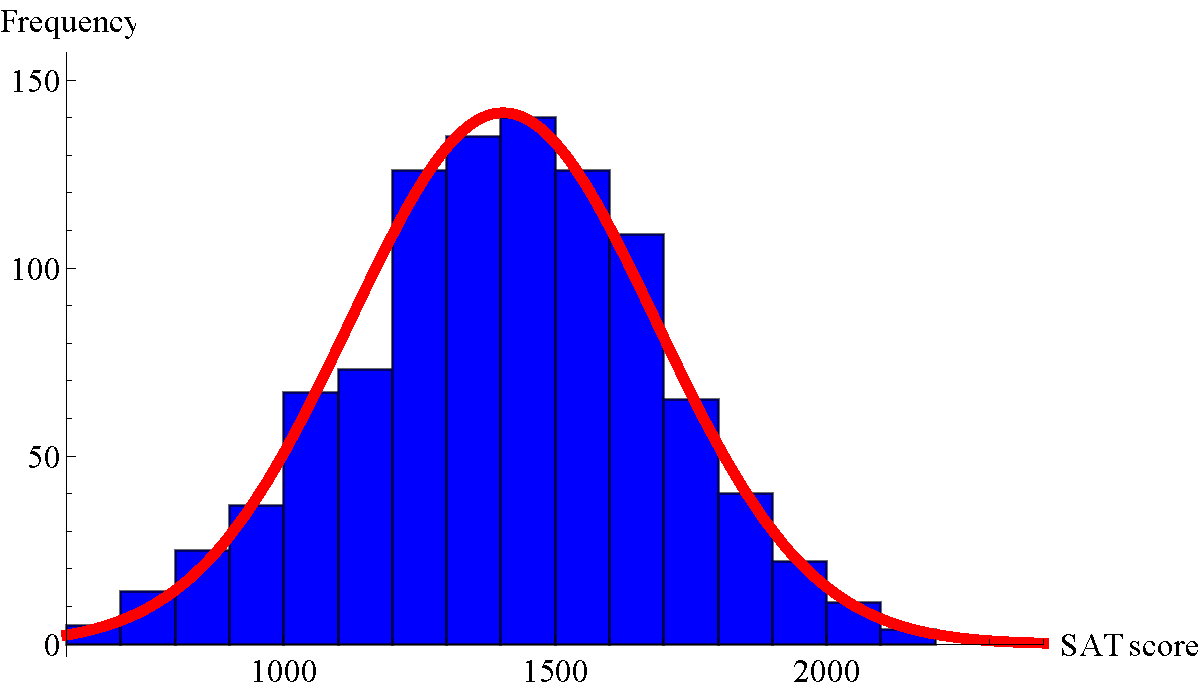
\includegraphics{Prior_SATScoresHistogram.pdf}}\caption{The SAT scores for past students of a class. The mean and variance of this hypothetical sample are 1404, and 79,716 respectively, which are used to fit a normal distribution to the data, and is shown in red.}\label{fig:Prior_SATScoresHistogram}
\end{figure}


Whilst this simple methodology can result in priors that closely approximate pre-experimental datasets, note that it was a arbitrary choice to fit the first two moments of the sample. We could have used the skewness and kurtosis (measures related to the third and fourth centred moments respectively). Also, moment-matching is not Bayesian in nature, and can often be difficult to apply in practice. When we discuss hierarchical models in chapter \ref{chap:hierarchicalModels}, we will learn a more pure Bayesian method which can be used to create prior densities.

\subsection{The numerator of Bayes' rule determines the shape}\label{sec:Prior_numerator}
We notice for both the examples described in sections \ref{sec:Prior_urn} and \ref{sec:Prior_diseaseProp} that the overall shape of the posterior distribution is determined by the prior, $P(\theta)$, multiplied by the likelihood, $P(data|\theta)$. This is the numerator of Bayes' rule:

\begin{equation}
P(\theta|data) = \frac{{\color{blue}P(\theta)\times P(data|\theta)}}{P(data)} \propto {\color{blue}P(\theta)\times P(data|\theta)}
\end{equation}\label{eq:Prior_BayesNumerator}

The shape of the posterior is determined by how it varies with $\theta$. Since the denominator is independent of $\theta$, the numerator completely describes how the gradient and curvature of the posterior density varies with $\theta$, which allows us to write the above  $ \propto {\color{blue}P(\theta)\times P(data|\theta)}$ statement. Viewed another way, the denominator is a nuisance normalisation factor which allows us to ensure that the posterior density when summed (discrete) or integrated (continuous) is equal to 1. We will return to a discussion of these concepts in depth in the chapter \ref{chap:denominator}, but it doesn't hurt to see where we may be headed at present.


\subsection{Eliciting priors}
A different sort of informative prior is often required, which is not derived from prior data, but from expert opinions. In particular these priors are often required for evaluating clinical trials, and clinicians are interviewed before the trial is conducted. However, there is a raft of research in the social sciences which also make use of these methods for prior construction. Whilst there are a plethora of methods for creating priors from subjective views (see \cite{gill2007bayesian} for a detailed discussion), we go through a simplified example in order to explain a potential way in which these methods are used. 

Suppose that we asked a range of economists to give their estimates of the 25th and 75th percentiles, ${wage}_{25}$ and ${wage}_{75}$, of the wage premium which one extra year of education spent at college commands on the job market on average. If we were to assume a normal prior for the data, then we can relate these two quantiles back to the corresponding values of a standardised normal distribution for each expert:

\begin{equation}\label{eq:Prior_elicitingPriorNormal}
\begin{align}
z_{25} &= \frac{{wage}_{25} - \mu}{\sigma}\\
z_{75} &= \frac{{wage}_{75} - \mu}{\sigma}
\end{align}
\end{equation}

In (\ref{eq:Prior_elicitingPriorNormal}), $z_{25}$ and $z_{50}$ are the 25th and 75th percentiles of the standard normal distribution respectively. These two simultaneous equations can be solved for each expert, giving an estimate of the mean and variance of a normal variable. These could then be averaged to get estimates of the mean and variance across all the experts. However, a better method relies on linear regression. The expressions in (\ref{eq:Prior_elicitingPriorNormal}) can be rearranged to the following:

\begin{equation}\label{eq:Prior_elicitingPriorNormalRegression}
\begin{align}
{wage}_{25} &= \mu + \sigma z_{25}\\
{wage}_{75} &= \mu + \sigma z_{75}
\end{align}
\end{equation}

We now recognise that each equation is of the form of a straight line $y = mx + c$, where in this case $c=\mu$ and $m=\sigma$. If we then fit a linear regression line to the data from all the panel, we can then use the values of the y-intercept and gradient for $\mu$ and $\sigma$ to estimate the mean and square root of the variance respectively (see figure \ref{fig:Prior_elicitingRegression}).

\begin{figure}
\centering
\scalebox{0.30} 
{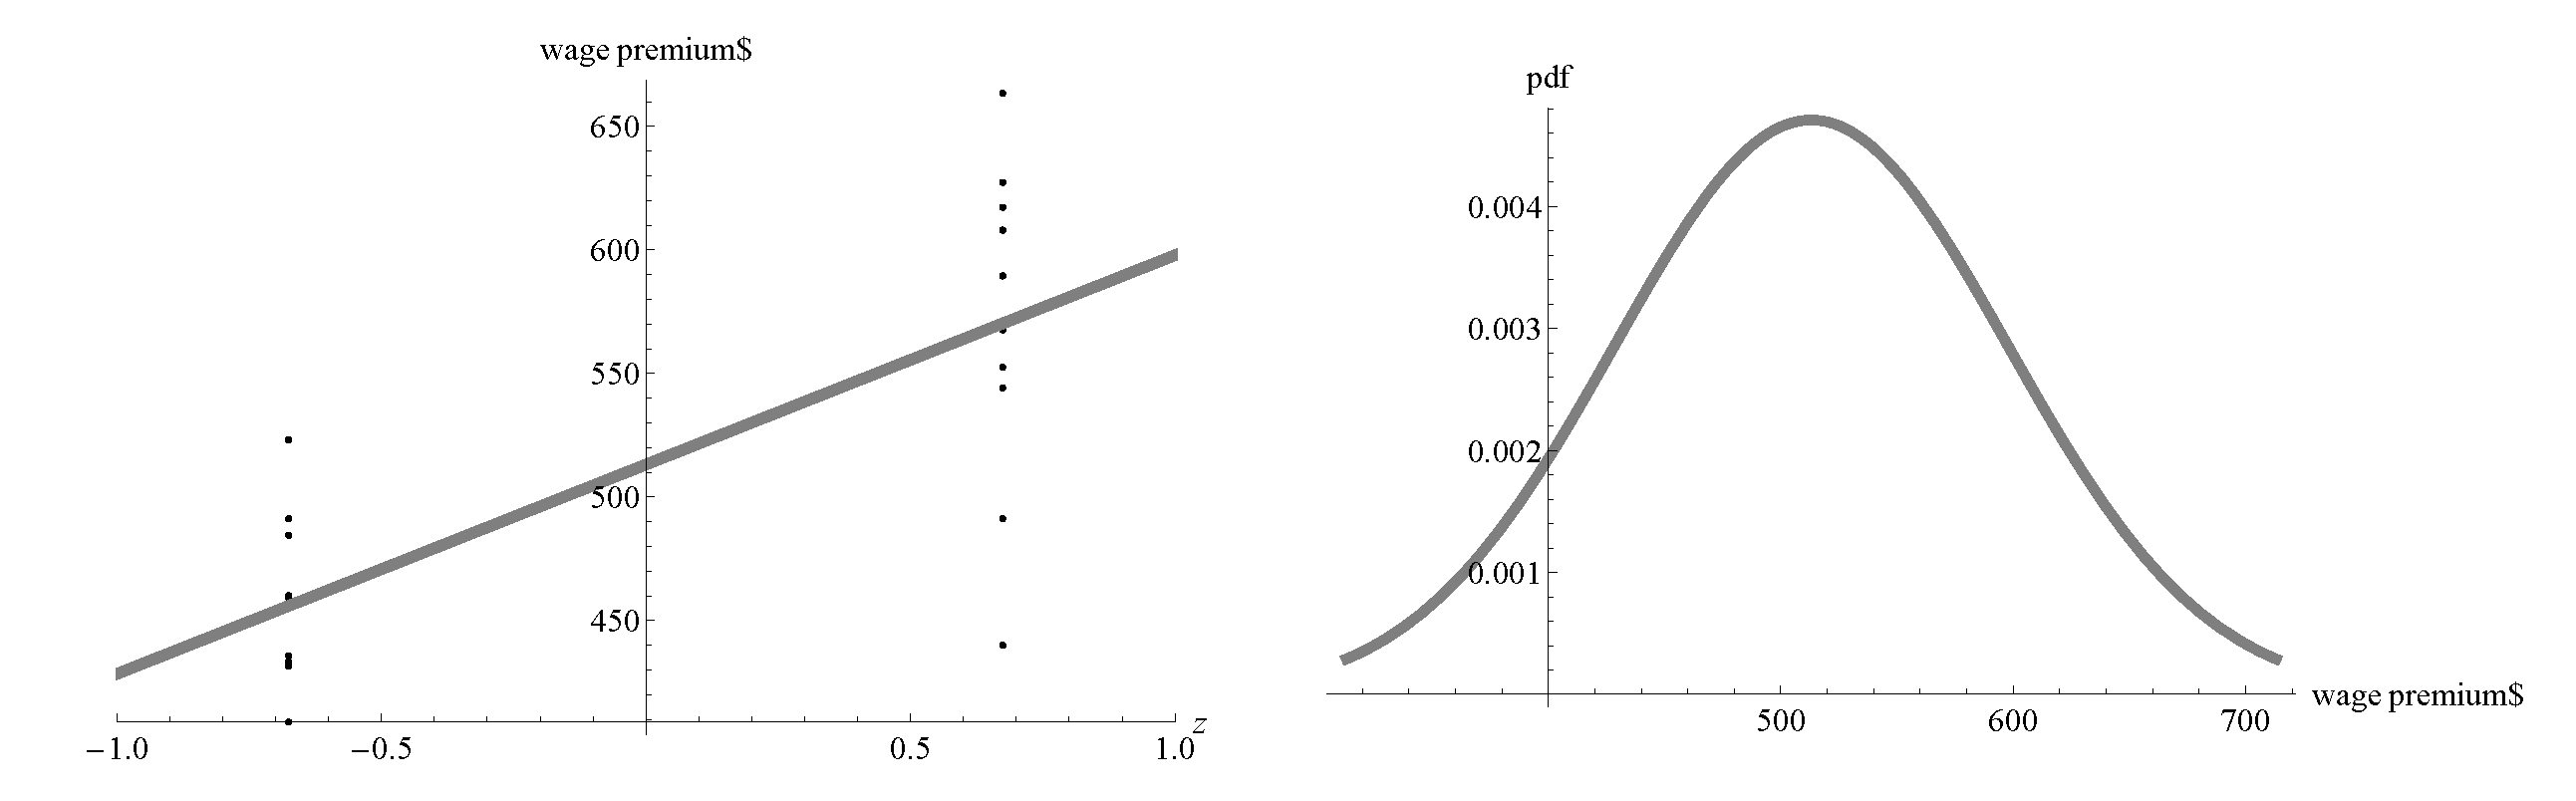
\includegraphics{Prior_elicitingRegression.pdf}}\caption{Hypothetical data for the 25th and 75th percentiles of the estimated wage premium from 10 experts. In the left hand panel we regress these percentiles on the corresponding percentiles from a standard normal distribution, yielding estimates of the mean and variance of a normal prior, which is shown on the right.}\label{fig:Prior_elicitingRegression}
\end{figure}

\section{A strong model is not heavily influenced by priors}
Returning to the example of section \ref{sec:Prior_diseaseProp} for estimated the prevalence of a disease within a population, we now examine the effects of using an informative prior on the analysis. Suppose we choose a prior which represents our pre-data view that the prevalence of a disease within a particular population is high (see the topmost row of figure \ref{fig:Prior_weakPriorEffect}). If we only have a sample size of 10, and obtain 1 individual in our sample who tests positive for the disease we see that the posterior is located roughly equidistant between the peaks of the prior and likelihood functions respectively (see the left hand column of figure \ref{fig:Prior_weakPriorEffect}). Now if we increase the sample size to 100, keeping the same percentage of individuals who are disease-positive within our sample, we then find that the posterior is peaked much closer to the position of the likelihood peak (see the middle column of figure \ref{fig:Prior_weakPriorEffect}). If we increase sample size further, maintaining the percentage of individuals with a disease in the sample, we see that the posterior peak's position appears indistinguishable from that of the likelihood (see the rightmost column of figure \ref{fig:Prior_weakPriorEffect}). 

We can see from figure \ref{fig:Prior_weakPriorEffect} that the effect of the prior on the posterior density decreases as we collect more data. Alternatively, we see that the likelihood - the effect of current data  - increases as we have access to further data points. This makes intuitive sense, since when we collect more evidence that comes solely from the data we should lend this source more weight, and pay less attention to our pre-experimental prejudices.

In general, in Bayesian analysis, when we collect more data our conclusions become less influenced by priors. The use of a prior allows us to make inferences in small sample sizes by using pre-experimental knowledge of a situation, but in larger samples, and for more appropriate models, we should see the effect of choice of priors decline. We have an obligation to report when choice of priors heavily influences the conclusions that we draw from an analysis, and \textit{sensitivity analysis} is a field which actually allows a range of priors to be specified, and combined into a single analysis. However, if we have sufficient data and a strong model, then we should see that the conclusions we draw are not heavily affected by choice of priors within a sensible range.

\begin{figure}
\centering
\scalebox{0.40} 
{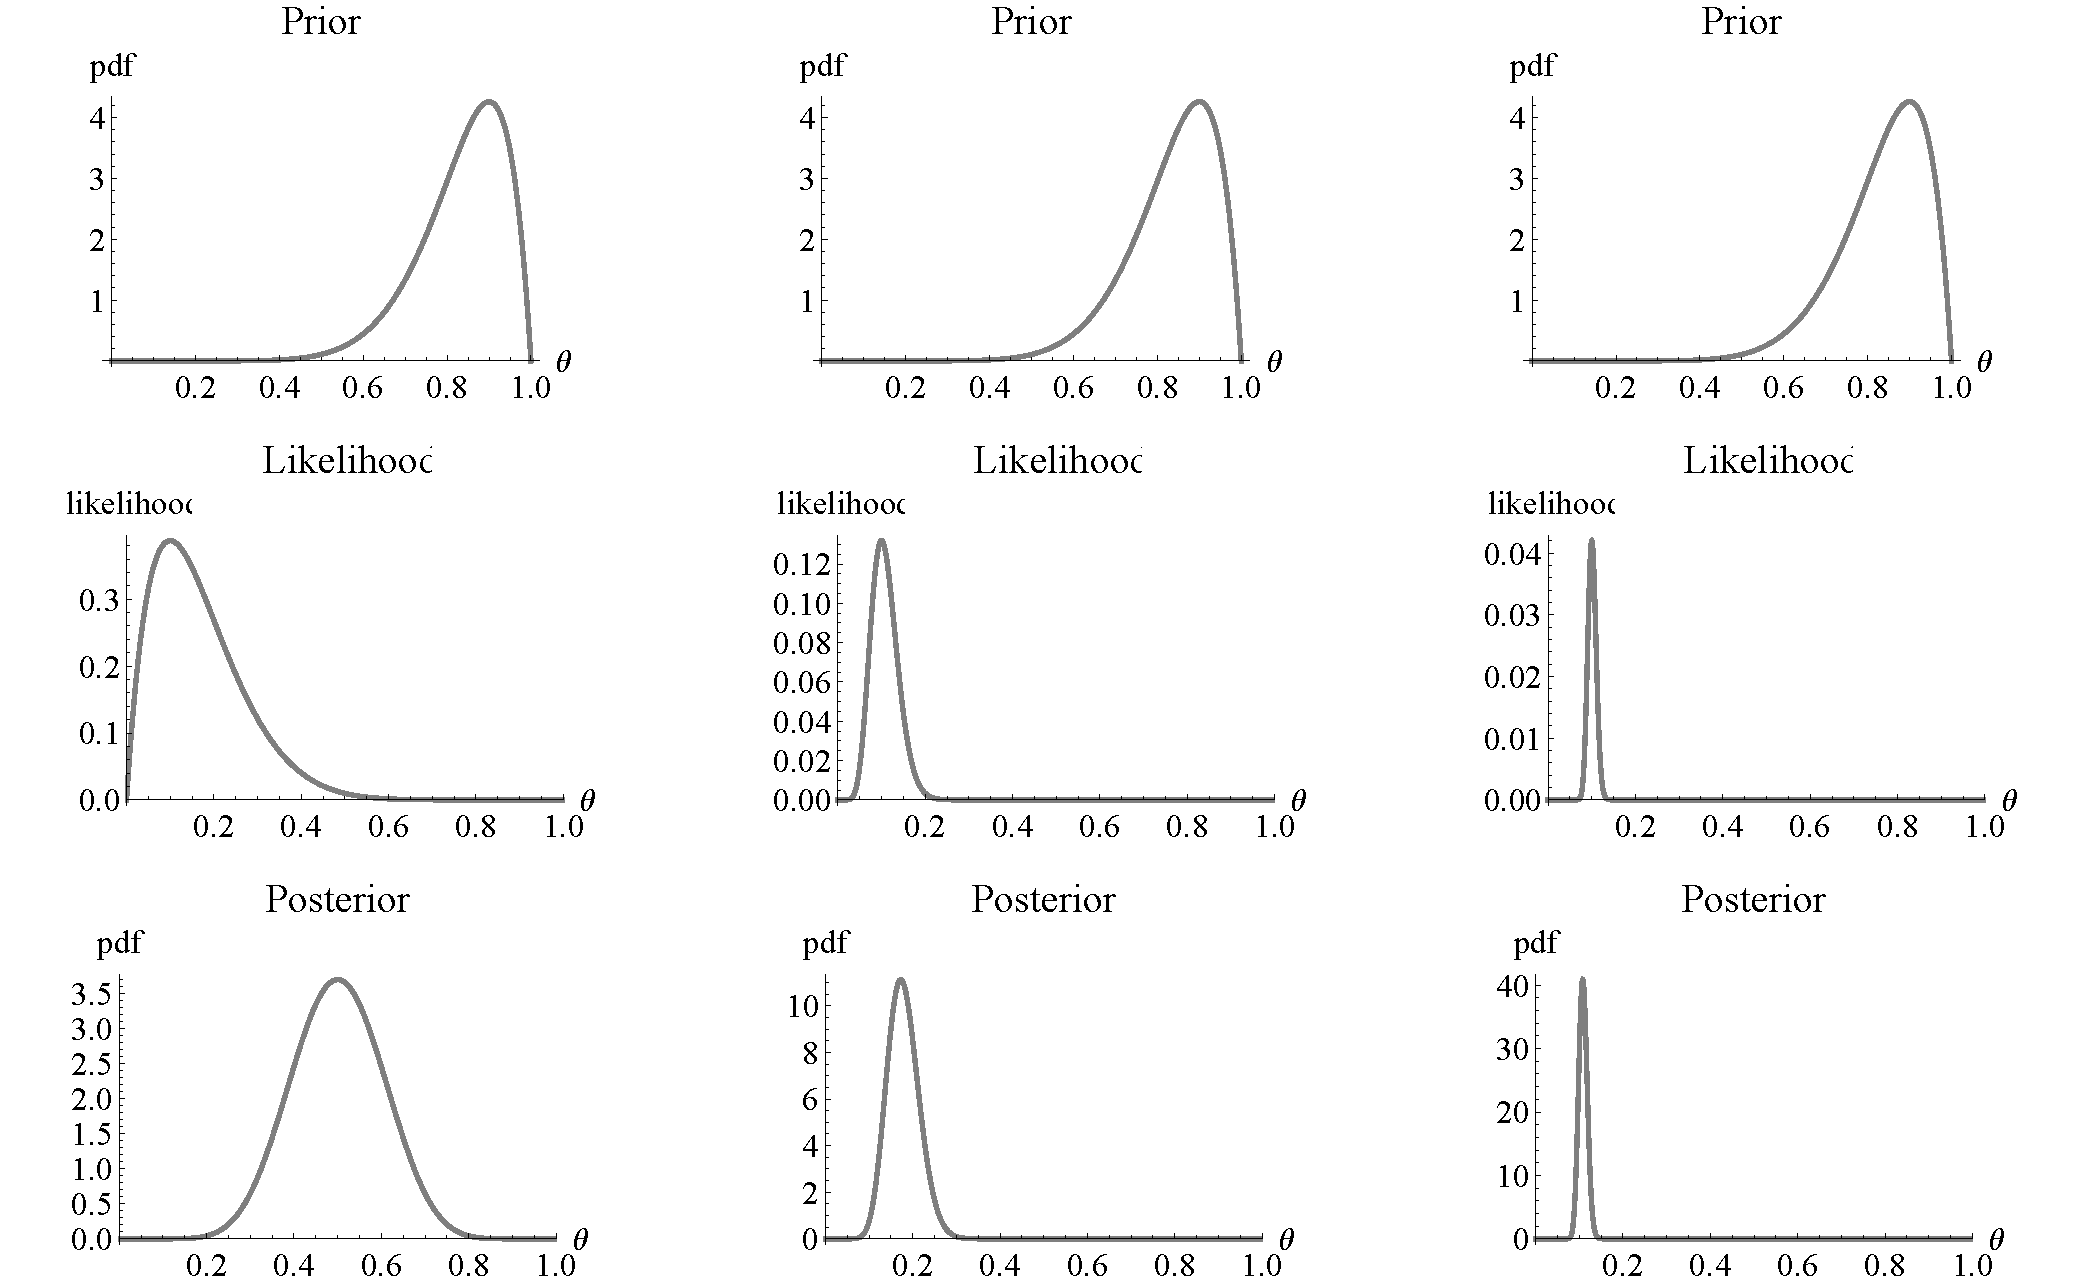
\includegraphics{Prior_weakPriorEffect.pdf}}\caption{The effect of increasing sample size on the posterior density for the prevalence of a disease in a population. The leftmost column has N=10, the middle N=100, and the rightmost N=1,000. All three have the same proportion of disease cases in the sample.}\label{fig:Prior_weakPriorEffect}
\end{figure}

\section{Chapter summary}
We now know that a \textit{prior} is a probability distribution that represents our pre-experimental/-data knowledge about a particular situation. We also understand the importance of selecting a proper prior density, and the need to test and interpret a posterior carefully that results from using an improper prior. Further we understand that when an emphasis is placed on drawing conclusions solely from the data, that a vague prior may be most appropriate. This contrasts with situations in which we wish to use pre-experimental data or expert knowledge to help us to draw conclusions, in which case we may choose a more informative prior. In all cases however, we realise the need to be aware of the how sensitive our inferences are to choice of prior. We also realise that as the amount of data increases, or a better model is chosen, then the posterior density is less sensitive to choice of prior.

We are now nearly in a position to start doing Bayesian analysis, all that we have left to cover is the denominator of Bayes' rule. This aspect appears relatively benign on first glances, but is actually where the difficulty lies in Bayesian approaches to inference. Appropriately then we devote the next chapter to studying this final part of Bayes' rule.

\section{Appendix}
\subsection{Bayes' rule for the urn}\label{app:Prior_bayesUrn}
In this case the application of the discrete form Bayes' rule takes the following form:

\begin{equation}\label{eq:Prior_bayesDiscreteForm}
\begin{align}
P(Y=\alpha|X=1) &= \frac{P(X=1|Y=\alpha)\times P(Y=\alpha)}{P(X=1)}\\
&= \frac{P(X=1|Y=\alpha)\times P(Y=\alpha)}{\sum\limits_{\alpha=0}^{5}P(X=1|Y=\alpha)\times P(Y=\alpha)}\\
&= \frac{\frac{\alpha}{5}\times \frac{1}{6}}{\sum\limits_{\alpha=0}^{5}\frac{\alpha}{5}\times\frac{1}{6}}
\end{align}
\end{equation}

\subsection{The probabilities of having a disease}\label{app:Prior_diseaseJeffreys}
We assume that the probability of an individual having a disease is $\theta$, and we assume a uniform prior on this probability, $P(\theta)=1$. We can calculate the probability that out of a sample of two, $P(Y)=P(\theta^2)$ by applying the change of variables rule:

\begin{equation}\label{eq:Prior_appChangeOfVariables}
P(Y) = P(\theta(Y))\times |\theta^\prime(Y)|
\end{equation}

In (\ref{eq:Prior_appChangeOfVariables}), $\theta(Y)=Y^{-\frac{1}{2}}$ is the inverse of $Y=\theta^2$, and $\theta^\prime$ means derivative wrt $Y$. Now substituting in this, we derive the probability density for two individuals having the disease:

\begin{equation}\label{eq:Prior_appChangeOfVariablesSolved}
P(Y) = \frac{1}{2\sqrt{Y}}
\end{equation}


\chapter{The devil's in the denominator}\label{chap:denominator}
\section{Chapter mission}
At the end of this chapter, the reader will understand what is represented by the denominator term, $P(data)$, in Bayes' rule. Furthermore, they will also have an appreciation of the inherent complexity of this term, as well as an idea of how modern computational methods can be used to bi-pass this.

Insert a graphic with the likelihood part of Bayes' formula circled, as in the equation shown below for the part highlighted in blue.

\begin{equation}
P(\theta|data) = \frac{P(data|\theta)\times P(\theta)}{{\color{blue}P(data)}}
\end{equation}\label{eq:Denominator_BayesHighlighted}


\section{Chapter goals}
Bayesian inference uses probability distributions, called \textit{posteriors}, to make inferences about the world at large. However, to be able to use these powerful tools, we must ensure they are probability distributions. The denominator of Bayes' rule, $P(data)$, ensures that the posterior distribution is a \textit{valid} probability distribution, by constraining the sum of its values to be 1. 

$P(data)$ is a marginal probability density obtained by a sum across all parameter values of the numerator. The seeming simplicity of the previous statement belies the fact that for many circumstances its calculation can be complicated, and often practically intractable. In this chapter we will learn the circumstances when this difficultly arises, as well as a basic appreciation as to how modern computational methods sidestep this issue. We will leave the details of how these methods work in practice to part \ref{part:computationalBayes}, but this chapter will lay the foundations for this later study.

\section{An introduction to the denominator}
\subsection{The denominator as a normalising factor}
We know from chapter \ref{chap:Likelihoods} that the likelihood is not a valid probability density, and hence we reason that the numerator of Bayes' rule - the likelihood multiplied by the prior - is similarly not constrained to be one either. The numerator will satisfy the first condition of a valid probability density: that its values are non-negative. However, the sum of the numerator across all parameter values will not generally be 1; meaning it fails the second test.

A natural way to normalise the numerator to ensure that the posterior is a valid probability density, is to divide by its sum; thus ensuring that its transformed variable's sum is always 1. The denominator of Bayes' rule, $P(data)$, is just this normalising factor. Notice that it does not contain the parameter, $\theta$. This is because $P(data)$ is a \textit{marginal} probability density (see section \ref{sec:Posterior_probabilityDistributions}), obtained by summing/integrating out all dependence on $\theta$. This parameter-independence of the denominator ensures that the dependence of the posterior distribution $P(\theta|data)$ on $\theta$ is solely through the numerator (see sections \ref{sec:Prior_numerator} and \ref{sec:Denominator_dispensingWithNumerator}). 

There are two varieties of Bayes' rule which we will employ in this chapter, which use slightly different\footnote{Although conceptually identical.} formulations of the denominator. When $\theta$ is a discrete parameter we are required to \textit{sum} over all possible parameter values, in order to obtain a factor which normalises the numerator:

\begin{equation}\label{eq:Denominator_discreteDenominator}
P(data) = \sum\limits_{All\;\theta} P(data|\theta) \times P(\theta)
\end{equation}

We will leave multiple-parameter inference largely to chapter $\ref{chap:conjugate}$, although will discuss how this leads to added complexity in section \ref{sec:Denominator_difficulty}. However, the method proceeds in an analogous manner to (\ref{eq:Denominator_discreteDenominator}), with the single sum replaced by a number of summations\footnote{The number of summations corresponds to the number of parameters in the model.}.

For continuous parameters we use the continuous analogue of the sum - an integral - resulting in a denominator of the form:

\begin{equation}\label{eq:Denominator_continuousDenominator}
P(data) = \int\limits_{All\;\theta} P(data|\theta) \times P(\theta) \mathrm{d}\theta
\end{equation}

Similarly, for multiple-parameter systems the single integral is replaced by a multiple-integral. We will now demonstrate how to use (\ref{eq:Denominator_discreteDenominator}) and (\ref{eq:Denominator_continuousDenominator}) through two examples in sections \ref{sec:Denominator_discreteExample} and \ref{sec:Denominator_continuousExample} respectively.

\subsection{Example: disease}\label{sec:Denominator_discreteExample}
Imagine that we are a medical practitioner tasked with evaluating the probability that a given patient has a particular disease. We use $\theta$ to represent the two possible outcomes: 

\begin{equation}
\theta =
\begin{cases}
O & , Disease \; negative \\
1 & ,  Disease \; positive
\end{cases}
\end{equation}

Using our experience and the patient's medical history we estimate that there is a probability of $\frac{1}{4}$ that this patient has the disorder; representing our prior. We then obtain test information, and are asked to re-evaluate the probability that the patient is disease-positive. In order to do this, we are required to state our likelihood. In this case we choose a likelihood of the form:

\begin{equation}\label{eq:Denominator_discreteLikelihood}
P(test\;positive|\theta) =
\begin{cases}
\frac{1}{10} & , \theta=0\\
\frac{4}{5} & ,  \theta=1
\end{cases}
\end{equation}

In (\ref{eq:Denominator_discreteLikelihood}), we implicitly assume that the probability of a negative test result is given by 1 minus the positive test probabilities. Also, by stating that there is a non-zero probability for $P(positive|\theta=0)$, we are assuming that false-positives do occur.

Suppose that the individual tests positive for the disease. We can now use (\ref{eq:Denominator_discreteDenominator}) to calculate the denominator of Bayes' rule in this case:

\begin{equation}
\begin{align}
P(test\; positive) &= \sum\limits_{\theta=0}^{1} P(test\; positive|\theta) \times P(\theta)\\
&= P(test\; positive|\theta=0) \times P(\theta=0) + P(test\; positive|\theta=1) \times P(\theta=1)\\
&= \frac{1}{10} \times \frac{3}{4} + \frac{4}{5} \times \frac{1}{4} = \frac{11}{40}
\end{align}
\end{equation}

Furthermore, it turns out the denominator is also a valid probability density\footnote{Due to the fact that we have removed the $\theta$ dependence that confounds attempts to view the numerator as one.}, meaning that we can calculate the counterfactual $P(test\; negative) = 1 - P(test\; positive) = \frac{29}{40}$. We need to be careful with interpreting this last result, since it didn't actually occur. It's best to think of $P(test\; negative)$ as the probability that we would assign to an individual testing negative before we carry out the test.

We can then use Bayes' rule to obtain the posterior probability that the individual has the disease, given that they tested positively:

\begin{equation}\label{eq:Denominator_discreteExamplePosterior}
\begin{align}
P(\theta=1|test\; positive) &= \frac{P(test\; positive|\theta=1)\times P(\theta=1)}{P(test\; positive)}\\
&= \frac{\frac{4}{5} \times \frac{1}{4}}{\frac{1}{10} \times \frac{3}{4} + \frac{4}{5} \times \frac{1}{4}}\\
&= \frac{8}{11}
\end{align}
\end{equation}

We see that in this case, even though we started off with a fairly optimistic prejudice - a probability that the individual has the disease of $\frac{1}{4}$ - the strength of the data has shone through, and we now are fairly confident of the alternative (see figure \ref{fig:Denominator_discreteExample} for a graphical depiction of this change of heart). Bayesians are fickle by design!

\begin{figure}
\centering
\scalebox{0.8} 
{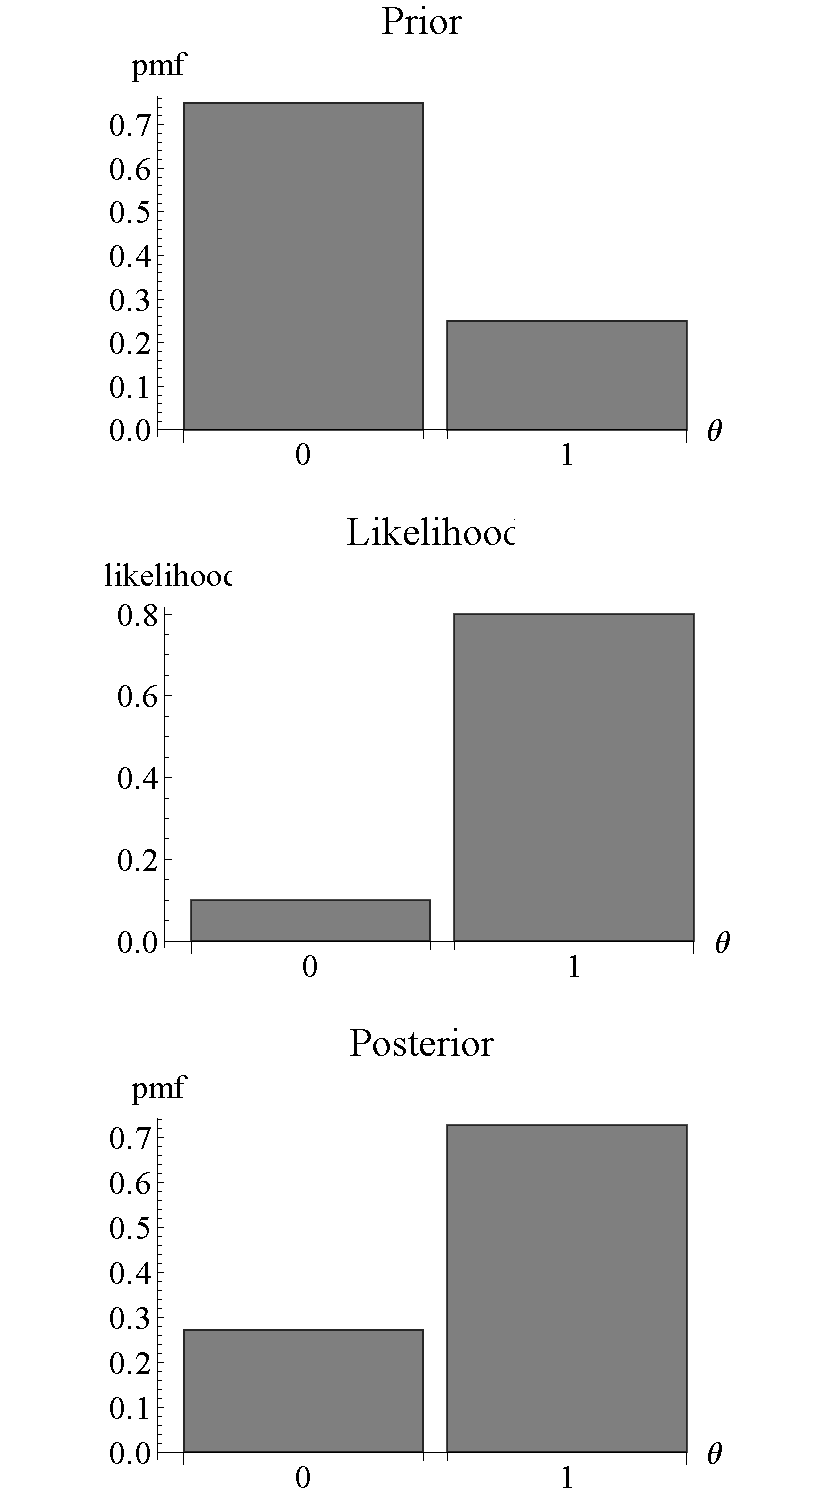
\includegraphics{Denominator_discreteExample.pdf}}\caption{The prior is multiplied through by the likelihood, resulting in the numerator (the penultimate panel), which is then normalised by the sum over its values, to obtain the denominator.}\label{fig:Denominator_discreteExample}
\end{figure}

\subsection{Example: the proportion of people who vote for conservatively}\label{sec:Denominator_continuousExample}
We now are in the position of interpreting exit polls in a general election, and are tasked with inferring the proportion of voters, $\theta$, that have voted for the conservative party. We suppose that conservatives are relatively unpopular at the time of the election, and hence we assume that, at most, 45\% of the electorate will vote for them, meaning we choose a cut-off uniform prior of the form shown in figure \ref{fig:Denominator_continuousExample}\footnote{This isn't really a reasonable prior in this case, since it is unrealistic to allow the probability density to jump from 0 at 46\% to above 2 at 45\%! However, we will stick with it to demonstrate its effect on inference.}. For data we obtain voter preference data from 100 individuals leaving a particular polling station. To simplify the analysis, we will assume that there are only two political parties, and all voters must choose between either of these two options. We will assume that the polling station chosen is thought to be representative of the electorate as a whole, and voters' choices are independent of one another. In this situation we can use the results of section \ref{sec:Likelihood_diseaseGroup}, and use a binomial likelihood function:

\begin{equation}\label{eq:Denominator_binomial}
P(Z=\beta|\theta) = {100 \choose \beta} \theta^\beta (1-\theta)^{100-\beta}
\end{equation}

In (\ref{eq:Denominator_binomial}), Z is a variable that represents the number of individuals who vote conservatively in the sample. $\beta\in[0,100]$ is the value which corresponds to the number of conservative voters. We assume in this case that 40 people out of the sample of 100 voted conservatively resulting in the likelihood shown in figure \ref{fig:Denominator_continuousExample}, which is peaked at the Maximum Likelihood estimate of $\theta=40\%$.

\begin{figure}
\centering
\scalebox{0.8} 
{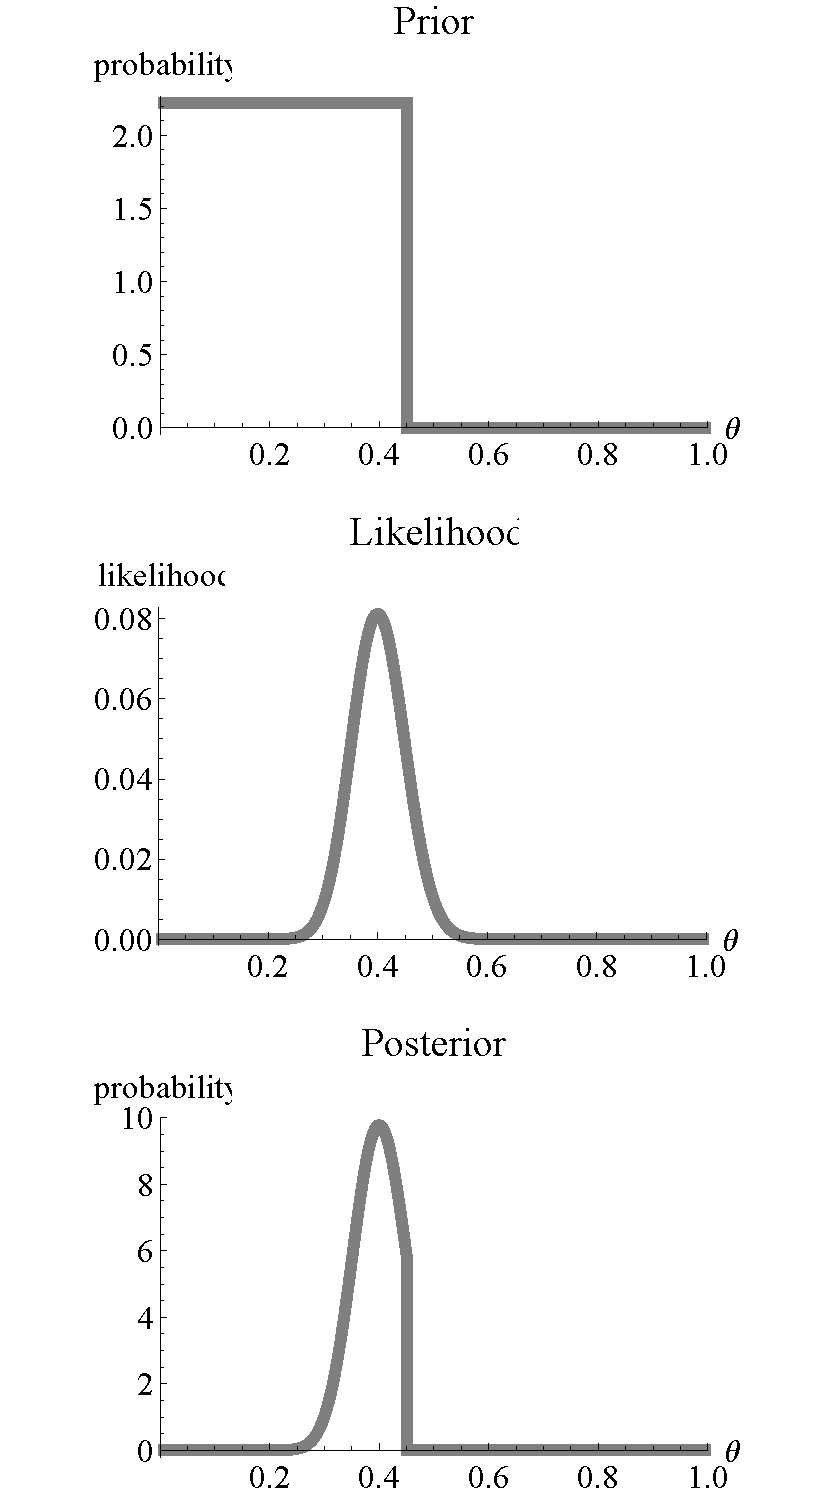
\includegraphics{Denominator_continuousExample.pdf}}\caption{The prior, likelihood and posterior for the proportion of individuals voting for the conservative party in a general election, where we have found 40 people out of a sample of 100 voted conservative.}\label{fig:Denominator_continuousExample}
\end{figure}

We then find the denominator by using (\ref{eq:Denominator_continuousDenominator}), where $\theta\in\{0,1\}$:

\begin{equation}\label{eq:Denominator_continuousExampleApprox}
\begin{align}
P(Z=40) &= \int\limits_{0}^{1} P(Z=40|\theta) \times P(\theta) \mathrm{d}\theta\\
&= \int\limits_{0}^{0.45} {100 \choose 40} \theta^{40} (1-\theta)^{60} \times \frac{20}{9} \mathrm{d}\theta\\
&\approx 0.018
\end{align}
\end{equation}

In (\ref{eq:Denominator_continuousExampleApprox}), we have used the fact that since $P(\theta)=0$ for $\theta>0.45$, we can restrict the integral to only the region below that value\footnotetext{The factor $\frac{20}{9}$ is from the uniform density for $\theta\leq 0.45$.}. The value $\theta\approx 0.018$ has come by numerically integrating the second line.

Now that we have the value of the denominator, we can use it to normalise the product of the prior and the likelihood, resulting in the posterior distribution seen in figure \ref{fig:Denominator_continuousExample}. Notice the effect of truncating the uniform distribution at $\theta=0.45$ is to truncate the posterior distribution at this value; resulting in a discontinuous jump in the posterior, which could be seen as an undesirable consequence of this prior.

\subsection{The denominator as a probability}\label{sec:Denominator_asAProbability}
Another way to view the denominator is as the \textit{probability of the data given choice of model}. Where \textit{model} here encompasses both the likelihood and the prior. It is actually a \textit{marginal} probability density that is obtained by summing/integrating out the dependence on the parameter(s) of the joint density $P(data,\theta)$:

\begin{equation}\label{eq:Denominator_jointDensity}
\begin{align}
p(data) &= \int\limits_{All\; \theta} p(data|\theta) \times p(\theta)\mathrm{d}\theta\\
& = \int\limits_{All\; \theta} p(data,\theta) \mathrm{d}\theta
\end{align}
\end{equation}

In (\ref{eq:Denominator_jointDensity}) we have assumed that the parameter(s) is/are continuous. We have obtained the second line of (\ref{eq:Denominator_jointDensity}) from the first by using the conditional probability formula introduced in section \ref{sec:Intro_probabilityDistributions}:

\begin{equation}
p(data|\theta) = \frac{p(data,\theta)}{p(\theta)}
\end{equation} 

We are thus able to characterise the joint density of the data and $\theta$ in Bayesian statistics. We can draw the joint density for each of the examples in sections \ref{sec:Denominator_discreteExample} and \ref{sec:Denominator_discreteExample} respectively, by taking the product of the likelihood and prior. In the disease example of section \ref{sec:Denominator_discreteExample} this results in the discrete joint density shown in table \ref{tab:Denominator_discreteJoint}, with a graphical depiction of the density shown in figure \ref{fig:Denominator_discreteJointDensity}. In the continuous case we obtain a joint probability density with a landscape of the form shown in figure \ref{fig:Denominator_continuousJointDensity}.


\begin{table}[htbp]
  \centering
  
    \begin{tabular}{rr|cccc}
    
     &       & \multicolumn{2}{c}{\textbf{Disease status}} \\
    \toprule
          & \textbf{Test Results} & \textbf{Negative} & \textbf{Positive} \\
          \midrule
\textbf{Likelihood} & \multicolumn{1}{c}{0}\vline & 0.90   & 0.20 \\
          & \multicolumn{1}{c}{1}\vline & 0.10   & 0.80 \\
          &       & \multicolumn{1}{r}{} & \multicolumn{1}{r}{} \\
          &       & $\times$ & $\times$ \\
          &       & \multicolumn{1}{r}{} & \multicolumn{1}{r}{} \\
    \textbf{Prior} &       & 0.75  & 0.25 \\
    &       & \multicolumn{1}{r}{} & \multicolumn{1}{r}{} \\
          & \textbf{} & \textbf{=} & \textbf{=} \\
&      \textbf{Test Results} & \multicolumn{1}{r}{} & \multicolumn{1}{r}{} & $p(data)$ \\
    \textbf{Joint density} & \multicolumn{1}{c}{0} \vline& 0.675 & 0.05  & \textbf{0.725}\\
          & \multicolumn{1}{c}{1}\vline & 0.075 & 0.20 & \textbf{0.275}\\
    \bottomrule
    \end{tabular}%
    \caption{Shows the derivation of the joint density for the disease example described in section \ref{sec:Denominator_discreteExample}. Each column of the likelihood - corresponding to a given disease status - is multiplied by the corresponding prior, resulting in the joint density. By summing the joint density across the different disease statuses of the patient, this results in $p(data)$. \textbf{Add pluses and equals to the calculation of $p(data)$. Also add in the posterior calculation.} See figure \ref{fig:Denominator_discreteJointDensity} for a graphical depiction of this joint density.}
  \label{tab:Denominator_discreteJoint}%
\end{table}%

\begin{figure}
\centering
\scalebox{0.8} 
{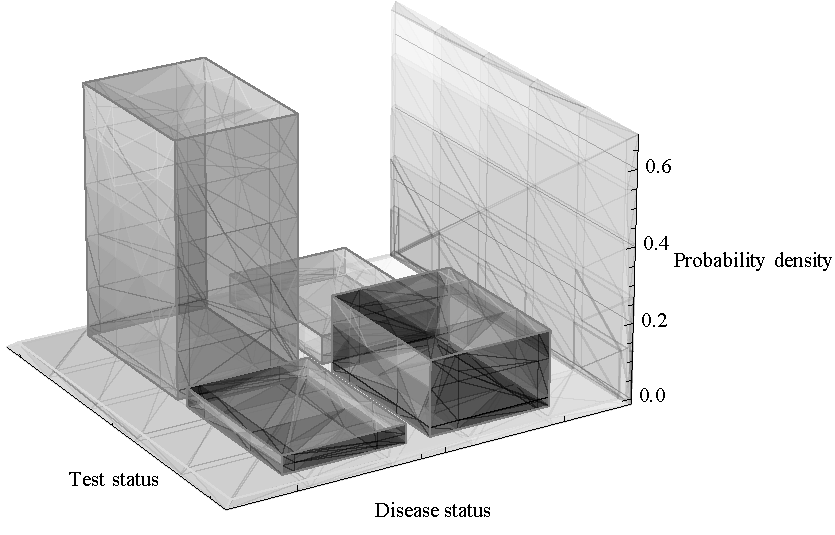
\includegraphics{Denominator_discreteJointDensity.pdf}}\caption{The joint density of the data and the parameter for the disease example described in section \ref{sec:Denominator_discreteExample}. When we uncover that the test result is positive, we are confined to look at the bars in dark grey; finding that the probability that an individual is diseased is significantly higher than the alternative (see the bottom panel of figure \ref{fig:Denominator_discreteExample}). \textbf{Perhaps redo this figure with a contour plot opposed to a 3D graph, and show how the posterior is obtained in another panel. Or just get rid of it, the table does pretty much cover it.}}\label{fig:Denominator_discreteJointDensity}
\end{figure}

\begin{figure}
\centering
\scalebox{0.8} 
{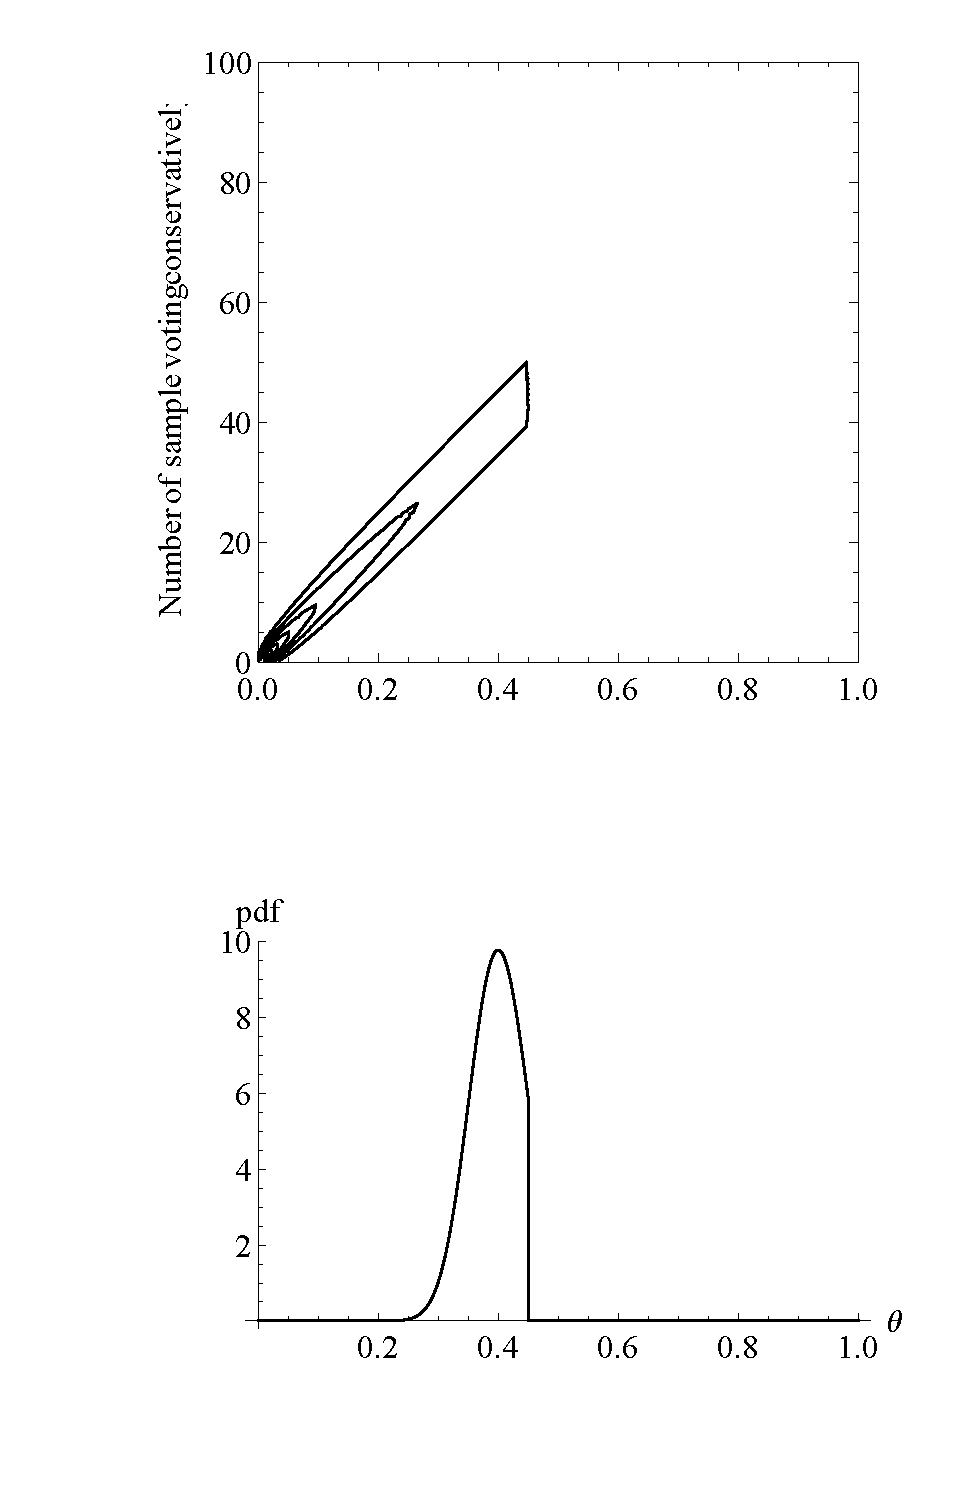
\includegraphics{Denominator_continuousJointDensity.pdf}}\caption{Top-left: a contour plot of the joint density of the voting example described in section \ref{fig:Denominator_continuousJointDensity}. Top-right: the marginal density of $p(data)$ obtained by summing across all values of $\theta$. Bottom-left: the posterior obtained by summing the joint density across the line shown at 40. Note that in reality the data variable is discrete, but I have drawn it here as continuous to make the plot simpler to interpret. \textbf{The line at 40 may be dashed in the final version. The axes all need to be aligned.}}\label{fig:Denominator_continuousJointDensity}
\end{figure}



\subsection{Using the denominator to choose between competing models}
The denominator represents the accumulation of evidence for our particular model, with the result being a trade-off between our the data and our pre-experimental pre-conceptions. It represents the \textit{average} fit of our model to the data across all parameter values. To see this note that the denominator is actually the expected value of the likelihood - the fit - given choice of prior\footnote{This comes from the mathematical definition of the expected value of a quantity.}:

\begin{equation}\label{eq:Denominator_expectedLikelihood}
p(data) = \mathbb{E}_\theta\left[p(data|\theta)\right] = \int\limits_{All\; \theta} p(data|\theta) \times p(\theta) \mathrm{d}\theta
\end{equation}

In (\ref{eq:Denominator_expectedLikelihood}) we have assumed that the parameter(s) are continuous, necessitating an integral rather than a discrete sum.

Since it really represents the evidence for our model, we can use it to compare two competing models. We could simply calculate the ratio of $\frac{p(data|model_1)}{p(data|model_2)}$, and use this as a guide to choose between models, but we would ideally like to do model selection in a more complete Bayesian manner. What we really care about for model choice is $p(model|data)$, rather than what we currently have $p(data|model)$. To obtain this we can use Bayes' rule, but now conditioning on choice of \textit{model} rather than \textit{parameter}:

\begin{equation}\label{eq:Denominator_modelProbability}
p(model|data) = \frac{p(data|model)\times p(model)}{p(data)}
\end{equation} 

In (\ref{eq:Denominator_modelProbability}), the denominator is \textit{not} the same as that which we see in our previous applications of Bayes' rule, and represents the probability of obtaining the data across \textit{all} models. Notice also that we also have introduced $p(model)$ which represents our prior faith in this particular model. We can now use (\ref{eq:Denominator_modelProbability}) to choose between two models by calculating the ratio:

\begin{equation}\label{eq:Denominator_modelComparison}
\frac{p(model_1|data)}{p(model_2|data)} = \frac{p(data|model_1)}{p(data|model_2)}\times \frac{p(model_1)}{p(model_2)}
\end{equation} 

If we have no prior leaning towards either of the two models then it seems reasonable to set $p(model_1)=p(model_2)$, and we are reduced to our previously proposed way of choosing between models. In fact the first ratio on the RHS of (\ref{eq:Denominator_modelComparison}) is sufficiently used to merit its own name, the \textit{Bayes' factor} is:

\begin{equation}\label{eq:Denominator_bayesFactor}
Bayes\; factor(model_1,model_2) = \frac{p(data|model_1)}{p(data|model_2)}
\end{equation}

We shall come to discuss the usefulness of the Bayes factor in chapter \ref{chap:ModelFit} for choosing between models, as well as comparing hypotheses.

In both the examples discussed in sections \ref{sec:Denominator_discreteExample} and \ref{sec:Denominator_continuousExample}, we found the denominator as a means to obtaining the posterior distribution through Bayes' rule. However, as an ends in itself it is less useful, unless it is calculated across a number of models/hypotheses and then used to choose amongst them.

\subsection{The denominator for improper priors}
The difficulty calculating P(data) with an improper prior.
Go through and correct P to p for probability.

\section{The difficulty with the denominator}\label{sec:Denominator_difficulty}
We have come to realise that the denominator of Bayes' rule is obtained by summing/integrating the joint density $p(data,\theta)$, where the latter is obtained by the product of the prior and the likelihood. The examples in section \ref{sec:Denominator_asAProbability} indicate how this procedure works when there is a single parameter in the model. However, in most real-life applications of statistics, the likelihood is a function of a number of parameters. For the case of a two parameter discrete model, the denominator is given by a double sum:

\begin{equation}\label{eq:Denominator_doubleSum}
p(data) = \sum\limits_{All\;\theta_1}\sum\limits_{All\;\theta_2}p(data,\theta_1,\theta_2)
\end{equation}

And for a two-dimensional continuous parameter vector, we are now required to do a double integral:

\begin{equation}\label{eq:Denominator_doubleIntegral}
p(data) = \int\limits_{All\;\theta_1}\int\limits_{All\;\theta_2}p(data,\theta_1,\theta_2)\mathrm{d}\theta_1\mathrm{d}\theta_2
\end{equation}

Whilst the two-parameter forms (\ref{eq:Denominator_doubleSum}) and (\ref{eq:Denominator_doubleIntegral}) may not look more intrinsically difficult than their single parameter counterparts, (\ref{eq:Denominator_discreteDenominator}) and (\ref{eq:Denominator_continuousDenominator}) respectively, this aesthetic similarity is misleading, particularly in the continuous case. Whilst in the discrete case, it is possible to enumerate all parameter values, and hence - by brute force - calculate the exact value of $p(data)$, for continuous parameters, the integral may be difficult to undertake. This difficulty is amplified the more parameters we include within the model, rendering the analytic\footnote{This just means to write down a relation for the denominator in closed form.} calculation of the denominator practically impossible, for all but the simplest models.

\subsection{Multi-parameter discrete model example: the comorbidity between depression and anxiety}\label{sec:Denominator_comorbidityTwoParameterDiscrete}
In medicine comorbidity refers to the concurrence of two or more conditions. An example of this is the frequent coincidence of depression and anxiety in a patient. Let $D\in\{0,1\}$ and $A\in\{0,1\}$ be random variables representing the depression and anxiety statuses of a particular patient respectively. Now that we have two parameters, we must specify a joint prior distribution. An example prior is shown at of the top of table \ref{tab:Denominator_comorbidityTwoParameterDiscrete}, in which we have also calculated the marginal prior distributions by summing over all values of the other variable. We suppose that \textit{a priori} the clinician undertaking this case believes that the patient is unlikely to meet all the criteria necessary for them to be defined as having both disorders, which is reflected in a prior probability of $p(D=1,A=1)=0.6$.

We can also use this joint distribution to calculate prior conditional probabilities. For example, we can calculate the probability that an individual has anxiety, \textit{given} that they have depression:

\begin{equation}
\begin{align}
p(A=1|D=1) &= \frac{p(A=1,D=1)}{p(D=1)}\\
&= \frac{0.2}{0.35}\\
&=\frac{4}{7}\approx 0.57
\end{align}
\end{equation}

This shows that it is considerably more likely that a patient has anxiety, if they are already depressed (compared with the unconditional $p(A=1)=0.25$), indicating our prior beliefs regarding the comorbidity of these two conditions.

We assume that the patient takes a personality diagnostic test which provides some extra information regarding whether the individual has either of these conditions. Let's assume for simplicity that the result of the test, $X\in\{0,1\}$, has the likelihood shown in the second panel of table \ref{tab:Denominator_comorbidityTwoParameterDiscrete}. The maximum likelihood estimator would be that the individual has $(D=1,A=1)$, with the lowest likelihood going to the disorder-free case.


\begin{table}[htbp]
  \centering
    \begin{tabular}{cccccc}
    \toprule
    \textbf{Prior} &       & \multicolumn{1}{c}{} & \multicolumn{2}{c}{\textbf{A}} &  \\
    
    \textbf{} &       & \multicolumn{1}{c}{} & \textbf{0} & \textbf{1} & \textbf{$p(D)$} \\
    \textbf{} & \textbf{D} & \multicolumn{1}{c}{\textbf{0}} & 0.6   & 0.05  & \textbf{0.65} \\
    \textbf{} &       & \multicolumn{1}{c}{\textbf{1}} & 0.15  & 0.2   & \textbf{0.35} \\
    \textbf{} &       & \multicolumn{1}{c}{\textbf{$p(A)$}} & \textbf{0.75} & \textbf{0.25} &  \\
    \midrule
    \textbf{Likelihood (X=1)} &       & \multicolumn{1}{c}{} & \multicolumn{2}{c}{\textbf{A}} &  \\
    \textbf{} &       & \multicolumn{1}{c}{} & \textbf{0} & \textbf{1} & \textbf{} \\
    \textbf{} & \textbf{D} & \multicolumn{1}{c}{\textbf{0}} & 0.05  & 0.4   & \textbf{} \\
    \textbf{} &       & \multicolumn{1}{c}{\textbf{1}} & 0.4   & 0.8   & \textbf{} \\
    \midrule
    \textbf{Numerator = Prior x Likelihood} &       & \multicolumn{1}{c}{} & \multicolumn{2}{c}{\textbf{A}} &  \\
    \textbf{} &       & \multicolumn{1}{c}{} & \textbf{0} & \textbf{1} &  \\
    \textbf{} & \textbf{D} & \multicolumn{1}{c}{\textbf{0}} & 0.03  & 0.02  &  \\
    \textbf{} & \textbf{} & \multicolumn{1}{c}{\textbf{1}} & 0.06  & 0.16  &  \\
    $\textbf{p(X=1)=0.03+0.03+0.06+0.16=0.27}$ &     &  &  &       &  \\
    \midrule
    \textbf{Posterior} &       & \multicolumn{1}{c}{} & \multicolumn{2}{c}{\textbf{A}} &  \\
          &       & \multicolumn{1}{c}{} & \textbf{0} & \textbf{1} & \textbf{$p(D|X=1)$} \\
          & \textbf{D} & \multicolumn{1}{c}{\textbf{0}} & 0.11  & 0.07  & \textbf{0.19} \\
          & \textbf{} & \multicolumn{1}{c}{\textbf{1}} & 0.22  & 0.59  & \textbf{0.81} \\
          &       & \multicolumn{1}{c}{\textbf{$p(A|X=1)$}} & \textbf{0.33} & \textbf{0.67} &  \\
    \bottomrule
    \end{tabular}%
    \caption{}
  \label{tab:Denominator_comorbidityTwoParameterDiscrete}%
\end{table}%

We would now like to calculate the joint posterior probability of the two conditions, given that an individual tests positive ($X=1$). We can write this using Bayes' rule, although now we must now make sure to condition the likelihood on both parameters. However, we can denote the parameter vector, $\boldsymbol{\theta}=(D,A)$, and apply Bayes' rule just as before:

\begin{equation}\label{eq:Denominator_TwoParameterDiscreteBayesSimple}
\begin{align}
p(\boldsymbol{\theta}|X=1) &= \frac{p(X=1|\boldsymbol{\theta})\times p(\boldsymbol{\theta})}{p(X=1)}\\
& = \frac{p(X=1|A,D)\times p(A,D)}{p(X=1)}
\end{align}
\end{equation}

In (\ref{eq:Denominator_TwoParameterDiscreteBayesSimple}), we have simply substituted the definition of, $\boldsymbol{\theta}=(D,A)$, into the top line to get the final expression. Therefore, just like before we multiply the likelihood by the prior to obtain the numerator of Bayes' rule. We finally sum over all numerator values, and use this to obtain the posterior distribution (see table \ref{tab:Denominator_comorbidityTwoParameterDiscrete}). In table \ref{tab:Denominator_comorbidityTwoParameterDiscrete} we have also calculated the marginal conditional posterior probabilities by using the law of conditional probability, and we find an 81 \% probability that the individual has depression, and 67 \% chance that they have anxiety. The probability that they have both disorders is 59\%.

\subsection{Continuous multi-parameter example: mean and variance of IQ}\label{sec:Denominator_continuousTwoParameterIQ}
We now consider a situation where the parameters of interest are continuous. It is hoped that this section will provide evidence for the complexity of analytic multi-parameter inference in Bayesian statistics, and hence by its very nature, the material covered here may be difficult to fully grasp. However, we will cover it in more detail in part \ref{part:analyticalBayes}.

We suppose we are interested in estimating the mean IQ of some population of interest, of which we only possess a sample of three persons' IQ data of $\boldsymbol{IQ}=\{100,50,150\}$. We suppose that since intelligence - as measured by $IQ$ - is dependent on many additive factors, and hence as an approximation we assume a normal likelihood\footnote{We have used the central limit theorem here - see section \ref{sec:Intro_CLT} for a full explanation.}:

\begin{equation}\label{eq:Denominator_continuousTwoParameterLikelihood}
p(IQ_i|\mu,\sigma^2) = \frac{1}{\sqrt{2\pi\sigma^2}} exp\left(-\frac{(IQ_i-\mu)^2}{2\sigma^2}\right)
\end{equation}

For sake of simplicity, we will assume that IQ is measured on a fixed scale, $IQ\in[0,300]$. We also assume that prior independence between $\mu$ and $\sigma^2$, which means that we can calculate the joint prior by multiplying together the individual probabilities:

\begin{equation}\label{sec:Denominator_continuousMultiparameterIndependence}
p(\mu,\sigma^2) = p(\mu) \times p(\sigma^2)
\end{equation}

Since $\sigma^2\geq 0$, we might be tempted to specify a prior distribution for $\sigma^2\sim Unif(0,\infty)$. However, this does not appear sensible because this would assign the same probability to an infinite variance, which is not possible on finite-scaled data. A frequently-used alternative is to specify a prior as uniform in $log(\sigma^2)$ space. This serves two purposes, firstly, because the inverse of a log (the exponent) is always non-negative for real inputs, this ensures that this condition is satisfied by $\sigma^2$. Secondly, and most importantly, when we transform a uniform prior on $log(\sigma^2)$ back to $\sigma^2$ space, we find that the prior density is equivalent to\footnote{See the chapter appendix for a full mathematical treatment of this result.}:

\begin{equation}\label{eq:Denominator_continuousTwoParameterPrior}
p(\sigma^2) \propto \frac{1}{\sigma^2}
\end{equation}

This results in a joint prior for $(\mu,\sigma^2)$ shown in figure \ref{fig:Denominator_continuousTwoParameter3D}. We importantly note that this prior is improper, since $\int\limits_{0}^{\infty} \frac{1}{\sigma^2}\mathrm{d}\sigma^2\rightarrow \infty$, and hence must take case when interpreting the resultant 'posterior' distribution (see section \ref{sec:Prior_vague}). 

\begin{figure}
\centering
\scalebox{0.25} 
{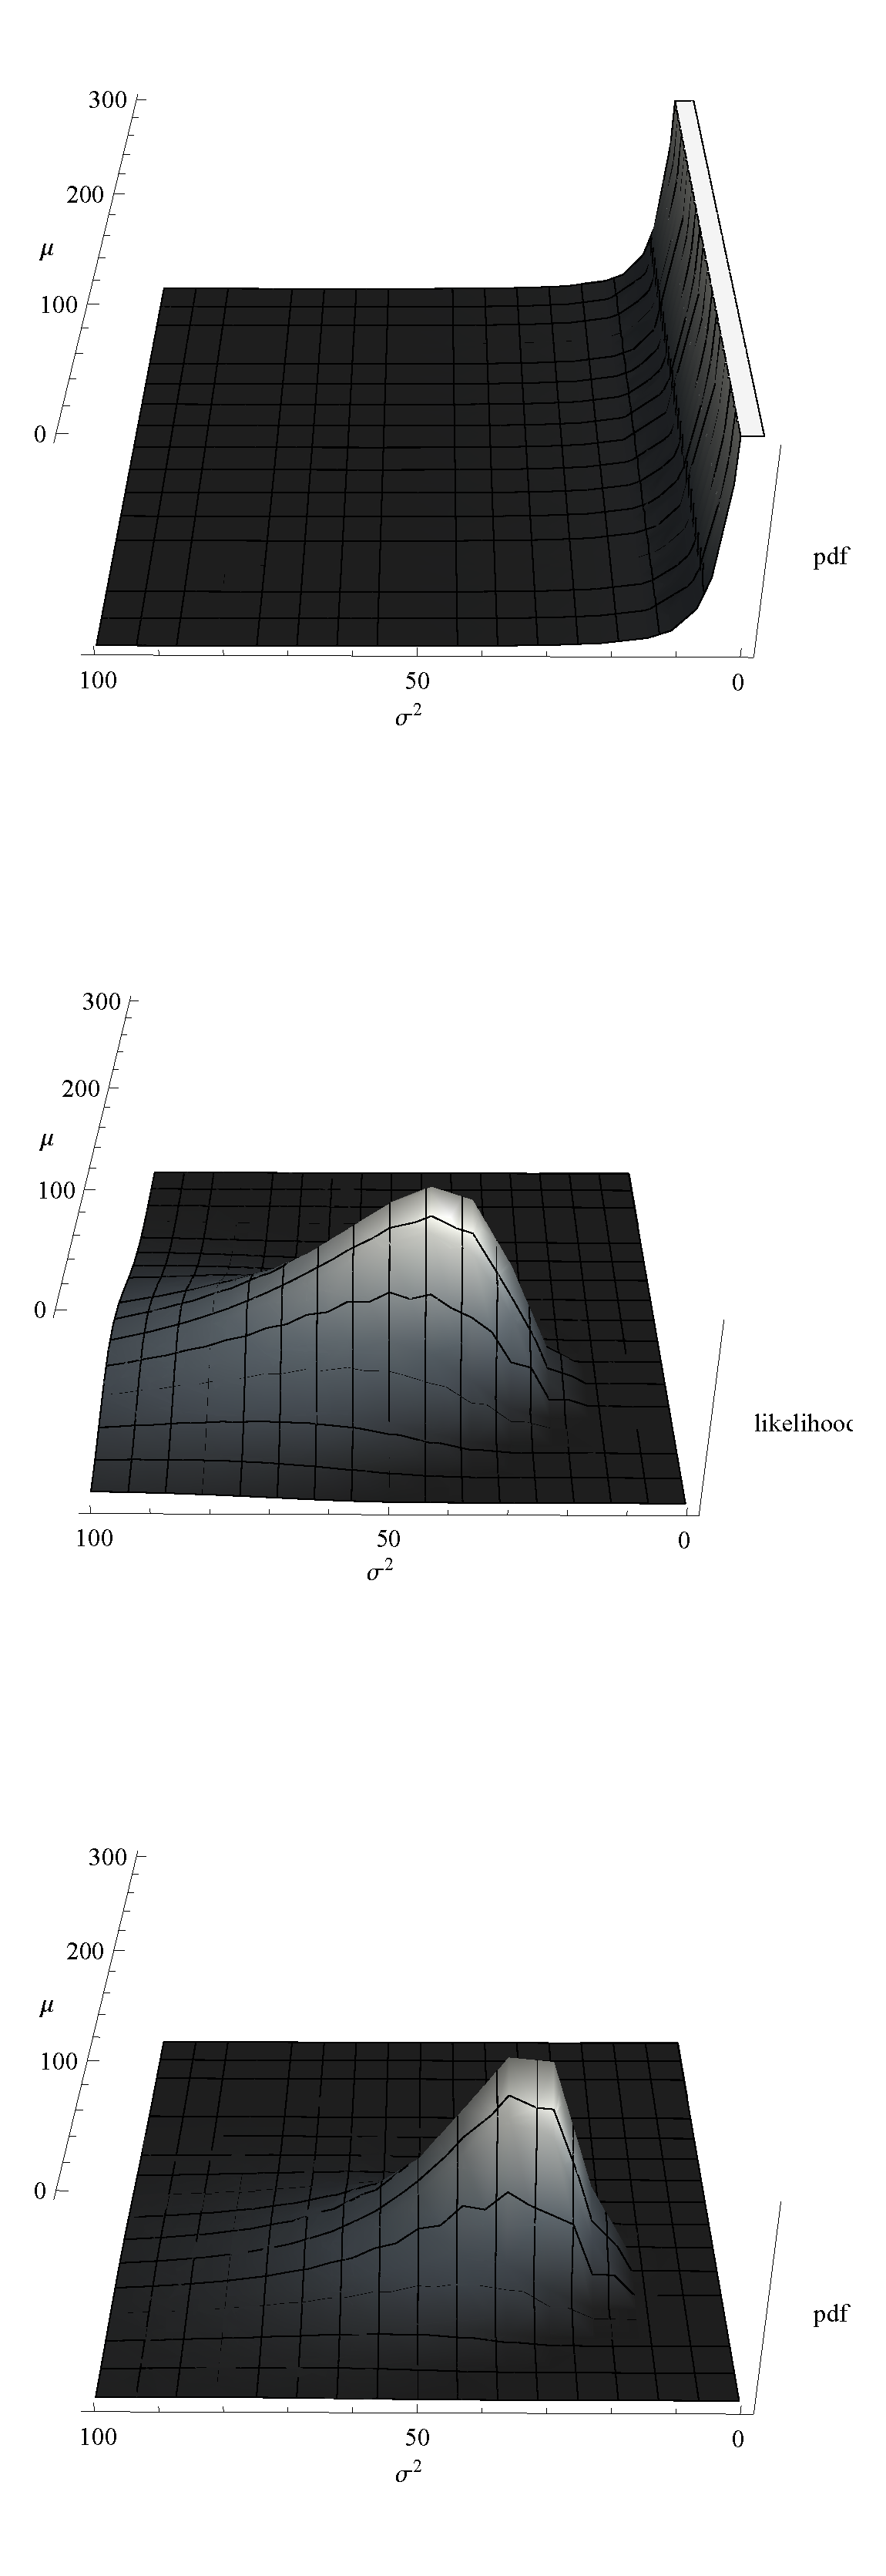
\includegraphics{Denominator_continuousTwoParameter3D.pdf}}\caption{The prior, likelihood, and posterior distributions for the mean and variance of IQ example described in section \ref{sec:Denominator_continuousTwoParameterIQ}.}}\label{fig:Denominator_continuousTwoParameter3D}
\end{figure}

We imagine we only observe a sample of one individual, from which we would like to find the posterior distribution of the joint distribution of $(\mu,\sigma^2)=\boldsymbol{\theta}$. This is found by application of Bayes' rule:

\begin{equation}\label{eq:Denominator_continuousTwoParameterJointPosterior}
\begin{align}
p(\boldsymbol{\theta}|\boldsymbol{IQ}) &= \frac{p(\boldsymbol{IQ}|\boldsymbol{\theta})\times p(\boldsymbol{\theta})}{p(\boldsymbol{IQ})}\\
&= \frac{p(\boldsymbol{IQ}|\mu,\sigma^2)\times p(\mu,\sigma^2)}{p(\boldsymbol{IQ})}\\
&= \frac{\frac{1}{\sqrt{2\pi\sigma^2}} exp\left(-\frac{\sum\limits_{i=1}^{3}(IQ_i-\mu)^2}{2\sigma^2}\right)\times\frac{1}{\sigma^2}}{\int\limits_{0}^{300}\int\limits_{0}^{\infty}\frac{1}{\sqrt{2\pi\sigma^2}} exp\left(-\frac{\sum\limits_{i=1}^{3}(IQ_i-\mu)^2}{2\sigma^2}\right)\times\frac{1}{\sigma^2}\mathrm{d}\sigma^2\mathrm{d}\mu}\\
&\propto \sigma^{-3} exp\left(-\frac{\sum\limits_{i=1}^{3}(IQ_i-\mu)^2}{2\sigma^2}\right)
\end{align}
\end{equation} 

In (\ref{eq:Denominator_continuousTwoParameterJointPosterior}), the second line was obtained from the first by simply substituting in for $\boldsymbol{\theta}=(\mu,\sigma^2)$. We then substituted for the likelihood\footnote{We have assumed independence for the data, meaning that to get the overall likelihood, we multiply together the three individual likelihoods.} and prior from (\ref{eq:Denominator_continuousTwoParameterLikelihood}) and (\ref{eq:Denominator_continuousTwoParameterPrior}) respectively. 

We can choose, in this rather simplified example, to go through and actually evaluate the posterior exactly, by calculating the denominator by brute force. This results in a posterior density shown in figures \ref{fig:Denominator_continuousTwoParameter3D} and \ref{fig:Denominator_continuousTwoParameterContour}. We can then obtain the marginal densities by integrating out any dependence of the parameter not in interest (see figure \ref{fig:Denominator_continuousTwoParameterContour}):


\begin{align}
p(\mu|\boldsymbol{IQ}) &= \int\limits_{0}^{\infty} p(\mu,\sigma^2|\boldsymbol{IQ}) \mathrm{d}\sigma^2\\
p(\sigma^2|\boldsymbol{IQ}) &= \int\limits_{0}^{300} p(\mu,\sigma^2|\boldsymbol{IQ}) \mathrm{d}\mu\\
\end{align}

Although, here we could go through and analytically derive the posteriors\footnote{Although we have chosen to omit the exact closed-form results here for brevity. Postponing such a full derivation until part \ref{part:analyticalBayes}.}, by evaluating the denominator, it is hoped that this example gives a little insight into the complexity of  calculating the denominator in Bayesian models. The degree of difficulty of calculating the denominator increases rapidly in the number of unknown parameters within a model. In fact, at some point, the denominator becomes practically infeasible to calculate for models more complicated than only a few parameters. 

However, all is not lost, as we discuss in section \ref{sec:Denominator_dispensingWithNumerator}.

\section{How to dispense with the difficulty: Bayesian computation}\label{sec:Denominator_dispensingWithNumerator}
The Herculean task of calculating the denominator for continuous parameters would seem to put a real spanner in the works for Bayesian statistics, such its reliance on the denominator of Bayes' rule. However, all is not lost. There are two solutions to the difficulty:

\begin{itemize}
\item Use priors conjugate to the likelihood (See chapter \ref{chap:conjugate}).
\item Abandon analyticity, and opt to sample from the posterior instead.
\end{itemize}

The first of these workarounds still allows for exact derivation of an expression for the posterior distribution, by choosing a mathematically \textit{nice} form for the prior distribution. This simplifies the analysis, since one can simply look up formulae for the posterior which have already been tabulated for us, avoiding to have to do any maths at all. However, frequently in real life applications of Bayesian statistics, we need to stray outside this realm of mathematical convenience. The price for a more varied choice of priors and likelihoods is that we have to give up our aspirations for closed-form calculation of the posterior density. However, it turns out in these circumstances we can still \textit{exactly} sample from the posterior, and then use sample summary statistics to describe the posterior distribution in a very adequate way. We will leave a full description of these computational methods to part \ref{part:computationalBayes}, but to provide a clue as to where we may be heading, we note that the posterior density can be written:

\begin{equation}\label{eq:Denominator_proportional}
\begin{align}
p(\theta|data) &= \frac{p(data|\theta)\times p(\theta)}{p(data)}\\
&\propto p(data|\theta)\times p(\theta)
\end{align}
\end{equation}

In (\ref{eq:Denominator_proportional}) we have arrived at the second line due to $p(data)$ being independent of $\theta$; it is essentially a constant that we use to normalise the posterior. The numerator of Bayes' rule tells us everything that we need to know about the \textit{shape}\footnote{It's dependence on $\theta$.} of the posterior distribution, whereas the denominator merely tells us about its \textit{height}. Computational methods use the shape of the posterior distribution to generate samples from it based on local comparison of relative probabilities. 

This provides a little insight into the methodology of modern Bayesian methods, although we will cover this in more depth in Part \ref{part:computationalBayes}. 

\section{Chapter summary}


\section{Appendix}\label{sec:Denominator_appendix}

\part{Analytic Bayesian methods}\label{part:analyticalBayes}
\chapter{An introduction to distributions for the mathematically-un-inclined}\label{chap:distributions}

\chapter{Conjugate priors and their place in Bayesian analysis}\label{chap:conjugate}

\chapter{Objective Bayesian analysis}\label{chap:ObjectiveBayes}

\part{A practical guide to doing real life Bayesian analysis: Computational Bayes}\label{part:computationalBayes}

\chapter{Hierarchical models}\label{chap:hierarchicalModels}

\part{Regression analysis and hierarchical models}
\chapter{Hypothesis testing I: Classical frequentist vs Bayesian approaches}

\chapter{Evaluation of model fit}\label{chap:ModelFit}
Formerly hypothesis testing II. Definitely use something similar to Kruscke's P67 example for choosing between models.

\bibliographystyle{plain}
\bibliography{Bayes}


\end{document}